%#########################1########################

 \cajita{%
Maíz }%
{%
 }%
{%
 Área cosechada y producción de maíz} %
{%
 República de Guatemala, serie histórica, en manzanas y  quintales } %
{%
 \begin{tikzpicture}[x=1pt,y=1pt]  % Created by tikzDevice version 0.9 on 2016-03-03 04:14:58
% !TEX encoding = UTF-8 Unicode
\definecolor{fillColor}{RGB}{255,255,255}
\path[use as bounding box,fill=fillColor,fill opacity=0.00] (0,0) rectangle (289.08,198.74);
\begin{scope}
\path[clip] (  0.00,  0.00) rectangle (289.08,198.74);

\path[] (  0.00,  0.00) rectangle (289.08,198.74);
\end{scope}
\begin{scope}
\path[clip] (  0.00,  0.00) rectangle (289.08,198.74);

\path[] (  0.00, 18.46) rectangle (289.08,142.27);

\path[] ( 33.36, 18.46) --
	( 33.36,142.27);

\path[] ( 88.95, 18.46) --
	( 88.95,142.27);

\path[] (144.54, 18.46) --
	(144.54,142.27);

\path[] (200.13, 18.46) --
	(200.13,142.27);

\path[] (255.72, 18.46) --
	(255.72,142.27);
\definecolor{drawColor}{RGB}{0,0,255}
\definecolor{fillColor}{RGB}{0,0,255}

\path[draw=drawColor,line width= 0.6pt,line join=round,fill=fillColor] (  9.73, 18.46) rectangle ( 31.97, 22.03);
\definecolor{drawColor}{RGB}{157,187,255}
\definecolor{fillColor}{RGB}{157,187,255}

\path[draw=drawColor,line width= 0.6pt,line join=round,fill=fillColor] ( 34.75, 18.46) rectangle ( 56.98,128.26);
\definecolor{drawColor}{RGB}{0,0,255}
\definecolor{fillColor}{RGB}{0,0,255}

\path[draw=drawColor,line width= 0.6pt,line join=round,fill=fillColor] ( 65.32, 18.46) rectangle ( 87.56, 22.11);
\definecolor{drawColor}{RGB}{157,187,255}
\definecolor{fillColor}{RGB}{157,187,255}

\path[draw=drawColor,line width= 0.6pt,line join=round,fill=fillColor] ( 90.34, 18.46) rectangle (112.57,130.74);
\definecolor{drawColor}{RGB}{0,0,255}
\definecolor{fillColor}{RGB}{0,0,255}

\path[draw=drawColor,line width= 0.6pt,line join=round,fill=fillColor] (120.91, 18.46) rectangle (143.15, 22.14);
\definecolor{drawColor}{RGB}{157,187,255}
\definecolor{fillColor}{RGB}{157,187,255}

\path[draw=drawColor,line width= 0.6pt,line join=round,fill=fillColor] (145.93, 18.46) rectangle (168.17,133.98);
\definecolor{drawColor}{RGB}{0,0,255}
\definecolor{fillColor}{RGB}{0,0,255}

\path[draw=drawColor,line width= 0.6pt,line join=round,fill=fillColor] (176.51, 18.46) rectangle (198.74, 22.21);
\definecolor{drawColor}{RGB}{157,187,255}
\definecolor{fillColor}{RGB}{157,187,255}

\path[draw=drawColor,line width= 0.6pt,line join=round,fill=fillColor] (201.52, 18.46) rectangle (223.76,138.78);
\definecolor{drawColor}{RGB}{0,0,255}
\definecolor{fillColor}{RGB}{0,0,255}

\path[draw=drawColor,line width= 0.6pt,line join=round,fill=fillColor] (232.10, 18.46) rectangle (254.33, 22.25);
\definecolor{drawColor}{RGB}{157,187,255}
\definecolor{fillColor}{RGB}{157,187,255}

\path[draw=drawColor,line width= 0.6pt,line join=round,fill=fillColor] (257.11, 18.46) rectangle (279.35,142.27);
\definecolor{drawColor}{RGB}{0,0,0}

\path[draw=drawColor,line width= 0.6pt,line join=round] (  0.00, 18.46) -- (289.08, 18.46);

\node[text=drawColor,rotate= 90.00,anchor=base west,inner sep=0pt, outer sep=0pt, scale=  0.83] at ( 24.08, 27.85) {1,175,255};

\node[text=drawColor,rotate= 90.00,anchor=base west,inner sep=0pt, outer sep=0pt, scale=  0.83] at ( 49.10,134.81) {36,117,212};

\node[text=drawColor,rotate= 90.00,anchor=base west,inner sep=0pt, outer sep=0pt, scale=  0.83] at ( 79.67, 27.93) {1,199,900};

\node[text=drawColor,rotate= 90.00,anchor=base west,inner sep=0pt, outer sep=0pt, scale=  0.83] at (104.69,137.29) {36,932,600};

\node[text=drawColor,rotate= 90.00,anchor=base west,inner sep=0pt, outer sep=0pt, scale=  0.83] at (135.27, 27.96) {1,211,900};

\node[text=drawColor,rotate= 90.00,anchor=base west,inner sep=0pt, outer sep=0pt, scale=  0.83] at (160.28,140.52) {37,995,900};

\node[text=drawColor,rotate= 90.00,anchor=base west,inner sep=0pt, outer sep=0pt, scale=  0.83] at (190.86, 28.03) {1,233,300};

\node[text=drawColor,rotate= 90.00,anchor=base west,inner sep=0pt, outer sep=0pt, scale=  0.83] at (215.88,145.33) {39,576,500};

\node[text=drawColor,rotate= 90.00,anchor=base west,inner sep=0pt, outer sep=0pt, scale=  0.83] at (246.45, 28.07) {1,247,100};

\node[text=drawColor,rotate= 90.00,anchor=base west,inner sep=0pt, outer sep=0pt, scale=  0.83] at (271.47,148.82) {40,724,100};

\path[] (  0.00, 18.46) rectangle (289.08,142.27);
\end{scope}
\begin{scope}
\path[clip] (  0.00,  0.00) rectangle (289.08,198.74);

\path[] (  0.00, 18.46) --
	(289.08, 18.46);
\end{scope}
\begin{scope}
\path[clip] (  0.00,  0.00) rectangle (289.08,198.74);

\path[] ( 33.36, 15.71) --
	( 33.36, 18.46);

\path[] ( 88.95, 15.71) --
	( 88.95, 18.46);

\path[] (144.54, 15.71) --
	(144.54, 18.46);

\path[] (200.13, 15.71) --
	(200.13, 18.46);

\path[] (255.72, 15.71) --
	(255.72, 18.46);
\end{scope}
\begin{scope}
\path[clip] (  0.00,  0.00) rectangle (289.08,198.74);
\definecolor{drawColor}{RGB}{0,0,0}

\node[text=drawColor,anchor=base,inner sep=0pt, outer sep=0pt, scale=  1.00] at ( 33.36,  5.69) {2010/2011};

\node[text=drawColor,anchor=base,inner sep=0pt, outer sep=0pt, scale=  1.00] at ( 88.95,  5.69) {2011/2012};

\node[text=drawColor,anchor=base,inner sep=0pt, outer sep=0pt, scale=  1.00] at (144.54,  5.69) {2012/2013};

<<<<<<< HEAD
\node[text=drawColor,anchor=base,inner sep=0pt, outer sep=0pt, scale=  1.00] at (200.13,  5.69) {2013/2014 \llamada};

\node[text=drawColor,anchor=base,inner sep=0pt, outer sep=0pt, scale=  1.00] at (255.72,  5.69) {2014/2015  \llamada};
=======
\node[text=drawColor,anchor=base,inner sep=0pt, outer sep=0pt, scale=  1.00] at (200.13,  5.69) {2013/2014 p};

\node[text=drawColor,anchor=base,inner sep=0pt, outer sep=0pt, scale=  1.00] at (255.72,  5.69) {2014/2015  e};
>>>>>>> origin/master
\end{scope}
\begin{scope}
\path[clip] (  0.00,  0.00) rectangle (289.08,198.74);
\coordinate (apoyo) at (61.96,191.07);
\coordinate (longitudFicticia) at (7.11,7.67);
\coordinate (longitud) at (7.11,7.11);
\coordinate (desX) at (128.08,0);
\coordinate (desY) at (0,0.28);
\definecolor[named]{ct1}{HTML}{
0000FF
}
\definecolor[named]{ct2}{HTML}{
9DBBFF
}
\definecolor[named]{ctb1}{HTML}{
0000FF
}
\definecolor[named]{ctb2}{HTML}{
9DBBFF
}
\path [fill=none] (apoyo) rectangle ($(apoyo)+(longitudFicticia)$)
node [xshift=0.3cm,inner sep=0pt, outer sep=0pt,midway,right,scale = 0.9]{Area};
\draw [color = ctb1,fill=ct1] ( $(apoyo)  + (desY) $) rectangle ($(apoyo)+ (desY) +(longitud)$);
\path [fill=none] ($(apoyo)+(desX)$) rectangle ($(apoyo)+(desX)+(longitudFicticia)$)
node [xshift=0.3cm,inner sep=0pt, outer sep=0pt,midway,right,scale = 0.9]{Producción};
\draw [color = ctb2 ,fill=ct2] ( $(apoyo)  + (desY) + (desX) $) rectangle ($(apoyo)+ (desY)+ (desX) +(longitud)$);
\end{scope}
  \end{tikzpicture}}%
{%
Diplan-MAGA con datos de Banguat (MAGA, 2013).} %


%#########################2########################

\cajita{%
	Rendimiento del maíz }%
{%
}%
{%
	Rendimiento del maíz } %
{%
	República de Guatemala, serie histórica, en quintales sobre manzanas } %
{%
	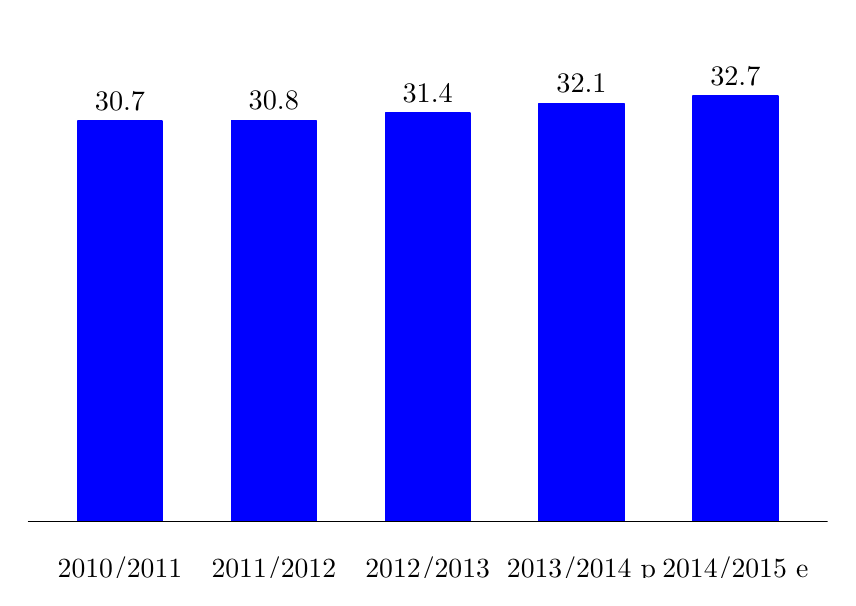
\begin{tikzpicture}[x=1pt,y=1pt]  % Created by tikzDevice version 0.9 on 2016-03-03 04:15:01
% !TEX encoding = UTF-8 Unicode
\definecolor{fillColor}{RGB}{255,255,255}
\path[use as bounding box,fill=fillColor,fill opacity=0.00] (0,0) rectangle (289.08,198.74);
\begin{scope}
\path[clip] (  0.00,  0.00) rectangle (289.08,198.74);

\path[] (  0.00,  0.00) rectangle (289.08,198.74);
\end{scope}
\begin{scope}
\path[clip] (  0.00,  0.00) rectangle (289.08,198.74);

\path[] (  0.00, 12.77) rectangle (289.08,181.67);

\path[] ( 33.36, 12.77) --
	( 33.36,181.67);

\path[] ( 88.95, 12.77) --
	( 88.95,181.67);

\path[] (144.54, 12.77) --
	(144.54,181.67);

\path[] (200.13, 12.77) --
	(200.13,181.67);

\path[] (255.72, 12.77) --
	(255.72,181.67);
\definecolor{drawColor}{RGB}{0,0,255}
\definecolor{fillColor}{RGB}{0,0,255}

\path[draw=drawColor,line width= 0.6pt,line join=round,fill=fillColor] ( 18.07, 20.44) rectangle ( 48.64,164.95);

\path[draw=drawColor,line width= 0.6pt,line join=round,fill=fillColor] ( 73.66, 20.44) rectangle (104.24,165.18);

\path[draw=drawColor,line width= 0.6pt,line join=round,fill=fillColor] (129.25, 20.44) rectangle (159.83,167.87);

\path[draw=drawColor,line width= 0.6pt,line join=round,fill=fillColor] (184.84, 20.44) rectangle (215.42,171.34);

\path[draw=drawColor,line width= 0.6pt,line join=round,fill=fillColor] (240.44, 20.44) rectangle (271.01,173.99);
\definecolor{drawColor}{RGB}{0,0,0}

\path[draw=drawColor,line width= 0.1pt,line join=round] (  0.00, 20.44) -- (289.08, 20.44);

\node[text=drawColor,anchor=base,inner sep=0pt, outer sep=0pt, scale=  1.02] at ( 33.36,168.92) {30.7};

\node[text=drawColor,anchor=base,inner sep=0pt, outer sep=0pt, scale=  1.02] at ( 88.95,169.15) {30.8};

\node[text=drawColor,anchor=base,inner sep=0pt, outer sep=0pt, scale=  1.02] at (144.54,171.84) {31.4};

\node[text=drawColor,anchor=base,inner sep=0pt, outer sep=0pt, scale=  1.02] at (200.13,175.31) {32.1};

\node[text=drawColor,anchor=base,inner sep=0pt, outer sep=0pt, scale=  1.02] at (255.72,177.96) {32.7};

\path[] (  0.00, 12.77) rectangle (289.08,181.67);
\end{scope}
\begin{scope}
\path[clip] (  0.00,  0.00) rectangle (289.08,198.74);

\path[] (  0.00, 12.77) --
	(289.08, 12.77);
\end{scope}
\begin{scope}
\path[clip] (  0.00,  0.00) rectangle (289.08,198.74);

\path[] ( 33.36, 10.02) --
	( 33.36, 12.77);

\path[] ( 88.95, 10.02) --
	( 88.95, 12.77);

\path[] (144.54, 10.02) --
	(144.54, 12.77);

\path[] (200.13, 10.02) --
	(200.13, 12.77);

\path[] (255.72, 10.02) --
	(255.72, 12.77);
\end{scope}
\begin{scope}
\path[clip] (  0.00,  0.00) rectangle (289.08,198.74);
\definecolor{drawColor}{RGB}{0,0,0}

\node[text=drawColor,anchor=base,inner sep=0pt, outer sep=0pt, scale=  1.00] at ( 33.36, -0.00) {2010/2011};

\node[text=drawColor,anchor=base,inner sep=0pt, outer sep=0pt, scale=  1.00] at ( 88.95, -0.00) {2011/2012};

\node[text=drawColor,anchor=base,inner sep=0pt, outer sep=0pt, scale=  1.00] at (144.54, -0.00) {2012/2013};

\node[text=drawColor,anchor=base,inner sep=0pt, outer sep=0pt, scale=  1.00] at (200.13, -0.00) {2013/2014 p};

\node[text=drawColor,anchor=base,inner sep=0pt, outer sep=0pt, scale=  1.00] at (255.72, -0.00) {2014/2015  e};
\end{scope}
  \end{tikzpicture}}%
{%
	Diplan-MAGA con datos de Banguat (MAGA, 2013).} %


%#########################3########################

\cajita{%
	Frijol }%
{%
}%
{%
	Área cosechada y producción de frijol} %
{%
	República de Guatemala, serie histórica, en manzanas y  quintales } %
{%
	\begin{tikzpicture}[x=1pt,y=1pt]  % Created by tikzDevice version 0.9 on 2016-03-03 04:15:01
% !TEX encoding = UTF-8 Unicode
\definecolor{fillColor}{RGB}{255,255,255}
\path[use as bounding box,fill=fillColor,fill opacity=0.00] (0,0) rectangle (289.08,198.74);
\begin{scope}
\path[clip] (  0.00,  0.00) rectangle (289.08,198.74);

\path[] (  0.00,  0.00) rectangle (289.08,198.74);
\end{scope}
\begin{scope}
\path[clip] (  0.00,  0.00) rectangle (289.08,198.74);

\path[] (  0.00, 18.46) rectangle (289.08,146.67);

\path[] ( 33.36, 18.46) --
	( 33.36,146.67);

\path[] ( 88.95, 18.46) --
	( 88.95,146.67);

\path[] (144.54, 18.46) --
	(144.54,146.67);

\path[] (200.13, 18.46) --
	(200.13,146.67);

\path[] (255.72, 18.46) --
	(255.72,146.67);
\definecolor{drawColor}{RGB}{0,0,255}
\definecolor{fillColor}{RGB}{0,0,255}

\path[draw=drawColor,line width= 0.6pt,line join=round,fill=fillColor] (  9.73, 18.46) rectangle ( 31.97, 26.79);
\definecolor{drawColor}{RGB}{157,187,255}
\definecolor{fillColor}{RGB}{157,187,255}

\path[draw=drawColor,line width= 0.6pt,line join=round,fill=fillColor] ( 34.75, 18.46) rectangle ( 56.98,132.55);
\definecolor{drawColor}{RGB}{0,0,255}
\definecolor{fillColor}{RGB}{0,0,255}

\path[draw=drawColor,line width= 0.6pt,line join=round,fill=fillColor] ( 65.32, 18.46) rectangle ( 87.56, 26.85);
\definecolor{drawColor}{RGB}{157,187,255}
\definecolor{fillColor}{RGB}{157,187,255}

\path[draw=drawColor,line width= 0.6pt,line join=round,fill=fillColor] ( 90.34, 18.46) rectangle (112.57,134.86);
\definecolor{drawColor}{RGB}{0,0,255}
\definecolor{fillColor}{RGB}{0,0,255}

\path[draw=drawColor,line width= 0.6pt,line join=round,fill=fillColor] (120.91, 18.46) rectangle (143.15, 27.00);
\definecolor{drawColor}{RGB}{157,187,255}
\definecolor{fillColor}{RGB}{157,187,255}

\path[draw=drawColor,line width= 0.6pt,line join=round,fill=fillColor] (145.93, 18.46) rectangle (168.17,138.35);
\definecolor{drawColor}{RGB}{0,0,255}
\definecolor{fillColor}{RGB}{0,0,255}

\path[draw=drawColor,line width= 0.6pt,line join=round,fill=fillColor] (176.51, 18.46) rectangle (198.74, 27.18);
\definecolor{drawColor}{RGB}{157,187,255}
\definecolor{fillColor}{RGB}{157,187,255}

\path[draw=drawColor,line width= 0.6pt,line join=round,fill=fillColor] (201.52, 18.46) rectangle (223.76,142.82);
\definecolor{drawColor}{RGB}{0,0,255}
\definecolor{fillColor}{RGB}{0,0,255}

\path[draw=drawColor,line width= 0.6pt,line join=round,fill=fillColor] (232.10, 18.46) rectangle (254.33, 27.32);
\definecolor{drawColor}{RGB}{157,187,255}
\definecolor{fillColor}{RGB}{157,187,255}

\path[draw=drawColor,line width= 0.6pt,line join=round,fill=fillColor] (257.11, 18.46) rectangle (279.35,146.67);
\definecolor{drawColor}{RGB}{0,0,0}

\path[draw=drawColor,line width= 0.6pt,line join=round] (  0.00, 18.46) -- (289.08, 18.46);

\node[text=drawColor,rotate= 90.00,anchor=base west,inner sep=0pt, outer sep=0pt, scale=  0.83] at ( 24.08, 31.51) {336,756};

\node[text=drawColor,rotate= 90.00,anchor=base west,inner sep=0pt, outer sep=0pt, scale=  0.83] at ( 49.10,138.37) {4,610,828};

\node[text=drawColor,rotate= 90.00,anchor=base west,inner sep=0pt, outer sep=0pt, scale=  0.83] at ( 79.67, 31.57) {339,200};

\node[text=drawColor,rotate= 90.00,anchor=base west,inner sep=0pt, outer sep=0pt, scale=  0.83] at (104.69,140.68) {4,704,200};

\node[text=drawColor,rotate= 90.00,anchor=base west,inner sep=0pt, outer sep=0pt, scale=  0.83] at (135.27, 31.73) {345,400};

\node[text=drawColor,rotate= 90.00,anchor=base west,inner sep=0pt, outer sep=0pt, scale=  0.83] at (160.28,144.17) {4,845,500};

\node[text=drawColor,rotate= 90.00,anchor=base west,inner sep=0pt, outer sep=0pt, scale=  0.83] at (190.86, 31.90) {352,500};

\node[text=drawColor,rotate= 90.00,anchor=base west,inner sep=0pt, outer sep=0pt, scale=  0.83] at (215.88,148.64) {5,026,200};

\node[text=drawColor,rotate= 90.00,anchor=base west,inner sep=0pt, outer sep=0pt, scale=  0.83] at (246.45, 32.05) {358,300};

\node[text=drawColor,rotate= 90.00,anchor=base west,inner sep=0pt, outer sep=0pt, scale=  0.83] at (271.47,152.49) {5,181,500};

\path[] (  0.00, 18.46) rectangle (289.08,146.67);
\end{scope}
\begin{scope}
\path[clip] (  0.00,  0.00) rectangle (289.08,198.74);

\path[] (  0.00, 18.46) --
	(289.08, 18.46);
\end{scope}
\begin{scope}
\path[clip] (  0.00,  0.00) rectangle (289.08,198.74);

\path[] ( 33.36, 15.71) --
	( 33.36, 18.46);

\path[] ( 88.95, 15.71) --
	( 88.95, 18.46);

\path[] (144.54, 15.71) --
	(144.54, 18.46);

\path[] (200.13, 15.71) --
	(200.13, 18.46);

\path[] (255.72, 15.71) --
	(255.72, 18.46);
\end{scope}
\begin{scope}
\path[clip] (  0.00,  0.00) rectangle (289.08,198.74);
\definecolor{drawColor}{RGB}{0,0,0}

\node[text=drawColor,anchor=base,inner sep=0pt, outer sep=0pt, scale=  1.00] at ( 33.36,  5.69) {2010/2011};

\node[text=drawColor,anchor=base,inner sep=0pt, outer sep=0pt, scale=  1.00] at ( 88.95,  5.69) {2011/2012};

\node[text=drawColor,anchor=base,inner sep=0pt, outer sep=0pt, scale=  1.00] at (144.54,  5.69) {2012/2013};

\node[text=drawColor,anchor=base,inner sep=0pt, outer sep=0pt, scale=  1.00] at (200.13,  5.69) {2013/2014 p};

\node[text=drawColor,anchor=base,inner sep=0pt, outer sep=0pt, scale=  1.00] at (255.72,  5.69) {2014/2015  e};
\end{scope}
\begin{scope}
\path[clip] (  0.00,  0.00) rectangle (289.08,198.74);
\coordinate (apoyo) at (61.96,191.07);
\coordinate (longitudFicticia) at (7.11,7.67);
\coordinate (longitud) at (7.11,7.11);
\coordinate (desX) at (128.08,0);
\coordinate (desY) at (0,0.28);
\definecolor[named]{ct1}{HTML}{
0000FF
}
\definecolor[named]{ct2}{HTML}{
9DBBFF
}
\definecolor[named]{ctb1}{HTML}{
0000FF
}
\definecolor[named]{ctb2}{HTML}{
9DBBFF
}
\path [fill=none] (apoyo) rectangle ($(apoyo)+(longitudFicticia)$)
node [xshift=0.3cm,inner sep=0pt, outer sep=0pt,midway,right,scale = 0.9]{Area};
\draw [color = ctb1,fill=ct1] ( $(apoyo)  + (desY) $) rectangle ($(apoyo)+ (desY) +(longitud)$);
\path [fill=none] ($(apoyo)+(desX)$) rectangle ($(apoyo)+(desX)+(longitudFicticia)$)
node [xshift=0.3cm,inner sep=0pt, outer sep=0pt,midway,right,scale = 0.9]{Producción};
\draw [color = ctb2 ,fill=ct2] ( $(apoyo)  + (desY) + (desX) $) rectangle ($(apoyo)+ (desY)+ (desX) +(longitud)$);
\end{scope}
  \end{tikzpicture}}%
{%
	MAGA.} %

%#########################4	########################

\cajita{%
	Frijol }%
{%
}%
{%
	Rendimiento del frijol} %
{%
	República de Guatemala, serie histórica, en quintales sobre manzanas } %
{%
	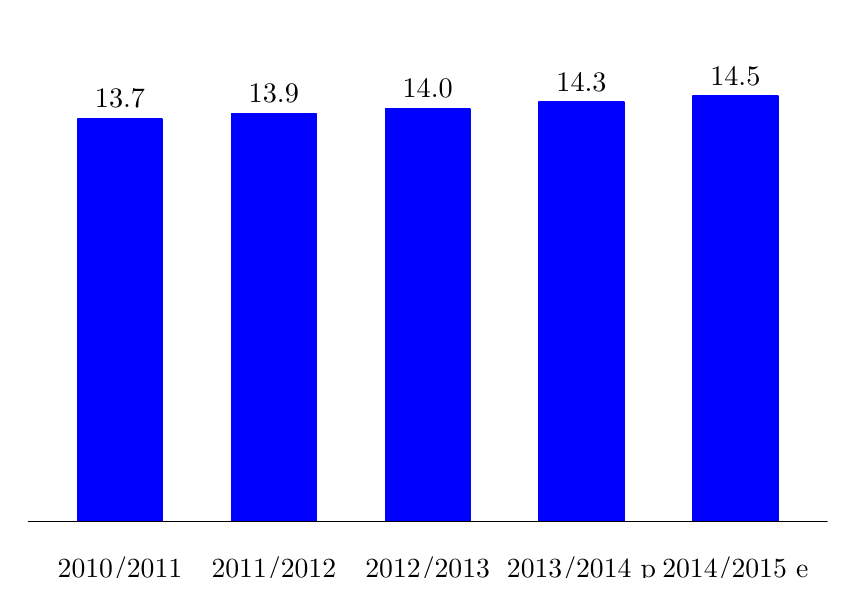
\begin{tikzpicture}[x=1pt,y=1pt]  % Created by tikzDevice version 0.9 on 2016-03-03 04:15:04
% !TEX encoding = UTF-8 Unicode
\definecolor{fillColor}{RGB}{255,255,255}
\path[use as bounding box,fill=fillColor,fill opacity=0.00] (0,0) rectangle (289.08,198.74);
\begin{scope}
\path[clip] (  0.00,  0.00) rectangle (289.08,198.74);

\path[] (  0.00,  0.00) rectangle (289.08,198.74);
\end{scope}
\begin{scope}
\path[clip] (  0.00,  0.00) rectangle (289.08,198.74);

\path[] (  0.00, 12.77) rectangle (289.08,181.67);

\path[] ( 33.36, 12.77) --
	( 33.36,181.67);

\path[] ( 88.95, 12.77) --
	( 88.95,181.67);

\path[] (144.54, 12.77) --
	(144.54,181.67);

\path[] (200.13, 12.77) --
	(200.13,181.67);

\path[] (255.72, 12.77) --
	(255.72,181.67);
\definecolor{drawColor}{RGB}{0,0,255}
\definecolor{fillColor}{RGB}{0,0,255}

\path[draw=drawColor,line width= 0.6pt,line join=round,fill=fillColor] ( 18.07, 20.44) rectangle ( 48.64,165.82);

\path[draw=drawColor,line width= 0.6pt,line join=round,fill=fillColor] ( 73.66, 20.44) rectangle (104.24,167.70);

\path[draw=drawColor,line width= 0.6pt,line join=round,fill=fillColor] (129.25, 20.44) rectangle (159.83,169.40);

\path[draw=drawColor,line width= 0.6pt,line join=round,fill=fillColor] (184.84, 20.44) rectangle (215.42,171.84);

\path[draw=drawColor,line width= 0.6pt,line join=round,fill=fillColor] (240.44, 20.44) rectangle (271.01,173.99);
\definecolor{drawColor}{RGB}{0,0,0}

\path[draw=drawColor,line width= 0.1pt,line join=round] (  0.00, 20.44) -- (289.08, 20.44);

\node[text=drawColor,anchor=base,inner sep=0pt, outer sep=0pt, scale=  1.02] at ( 33.36,169.79) {13.7};

\node[text=drawColor,anchor=base,inner sep=0pt, outer sep=0pt, scale=  1.02] at ( 88.95,171.67) {13.9};

\node[text=drawColor,anchor=base,inner sep=0pt, outer sep=0pt, scale=  1.02] at (144.54,173.37) {14.0};

\node[text=drawColor,anchor=base,inner sep=0pt, outer sep=0pt, scale=  1.02] at (200.13,175.81) {14.3};

\node[text=drawColor,anchor=base,inner sep=0pt, outer sep=0pt, scale=  1.02] at (255.72,177.96) {14.5};

\path[] (  0.00, 12.77) rectangle (289.08,181.67);
\end{scope}
\begin{scope}
\path[clip] (  0.00,  0.00) rectangle (289.08,198.74);

\path[] (  0.00, 12.77) --
	(289.08, 12.77);
\end{scope}
\begin{scope}
\path[clip] (  0.00,  0.00) rectangle (289.08,198.74);

\path[] ( 33.36, 10.02) --
	( 33.36, 12.77);

\path[] ( 88.95, 10.02) --
	( 88.95, 12.77);

\path[] (144.54, 10.02) --
	(144.54, 12.77);

\path[] (200.13, 10.02) --
	(200.13, 12.77);

\path[] (255.72, 10.02) --
	(255.72, 12.77);
\end{scope}
\begin{scope}
\path[clip] (  0.00,  0.00) rectangle (289.08,198.74);
\definecolor{drawColor}{RGB}{0,0,0}

\node[text=drawColor,anchor=base,inner sep=0pt, outer sep=0pt, scale=  1.00] at ( 33.36, -0.00) {2010/2011};

\node[text=drawColor,anchor=base,inner sep=0pt, outer sep=0pt, scale=  1.00] at ( 88.95, -0.00) {2011/2012};

\node[text=drawColor,anchor=base,inner sep=0pt, outer sep=0pt, scale=  1.00] at (144.54, -0.00) {2012/2013};

\node[text=drawColor,anchor=base,inner sep=0pt, outer sep=0pt, scale=  1.00] at (200.13, -0.00) {2013/2014 p};

\node[text=drawColor,anchor=base,inner sep=0pt, outer sep=0pt, scale=  1.00] at (255.72, -0.00) {2014/2015  e};
\end{scope}
  \end{tikzpicture}}%
{%
	MAGA.} %

%#########################5########################

\cajita{%
	Arroz }%
{%
}%
{%
	Área cosechada y producción de arroz} %
{%
	República de Guatemala, serie histórica, en manzanas y  quintales } %
{%
	\begin{tikzpicture}[x=1pt,y=1pt]  % Created by tikzDevice version 0.9 on 2016-03-03 04:15:04
% !TEX encoding = UTF-8 Unicode
\definecolor{fillColor}{RGB}{255,255,255}
\path[use as bounding box,fill=fillColor,fill opacity=0.00] (0,0) rectangle (289.08,198.74);
\begin{scope}
\path[clip] (  0.00,  0.00) rectangle (289.08,198.74);

\path[] (  0.00,  0.00) rectangle (289.08,198.74);
\end{scope}
\begin{scope}
\path[clip] (  0.00,  0.00) rectangle (289.08,198.74);

\path[] (  0.00, 18.46) rectangle (289.08,153.33);

\path[] ( 33.36, 18.46) --
	( 33.36,153.33);

\path[] ( 88.95, 18.46) --
	( 88.95,153.33);

\path[] (144.54, 18.46) --
	(144.54,153.33);

\path[] (200.13, 18.46) --
	(200.13,153.33);

\path[] (255.72, 18.46) --
	(255.72,153.33);
\definecolor{drawColor}{RGB}{0,0,255}
\definecolor{fillColor}{RGB}{0,0,255}

\path[draw=drawColor,line width= 0.6pt,line join=round,fill=fillColor] (  9.73, 18.46) rectangle ( 31.97, 21.22);
\definecolor{drawColor}{RGB}{157,187,255}
\definecolor{fillColor}{RGB}{157,187,255}

\path[draw=drawColor,line width= 0.6pt,line join=round,fill=fillColor] ( 34.75, 18.46) rectangle ( 56.98,138.65);
\definecolor{drawColor}{RGB}{0,0,255}
\definecolor{fillColor}{RGB}{0,0,255}

\path[draw=drawColor,line width= 0.6pt,line join=round,fill=fillColor] ( 65.32, 18.46) rectangle ( 87.56, 21.25);
\definecolor{drawColor}{RGB}{157,187,255}
\definecolor{fillColor}{RGB}{157,187,255}

\path[draw=drawColor,line width= 0.6pt,line join=round,fill=fillColor] ( 90.34, 18.46) rectangle (112.57,141.81);
\definecolor{drawColor}{RGB}{0,0,255}
\definecolor{fillColor}{RGB}{0,0,255}

\path[draw=drawColor,line width= 0.6pt,line join=round,fill=fillColor] (120.91, 18.46) rectangle (143.15, 21.29);
\definecolor{drawColor}{RGB}{157,187,255}
\definecolor{fillColor}{RGB}{157,187,255}

\path[draw=drawColor,line width= 0.6pt,line join=round,fill=fillColor] (145.93, 18.46) rectangle (168.17,144.77);
\definecolor{drawColor}{RGB}{0,0,255}
\definecolor{fillColor}{RGB}{0,0,255}

\path[draw=drawColor,line width= 0.6pt,line join=round,fill=fillColor] (176.51, 18.46) rectangle (198.74, 21.35);
\definecolor{drawColor}{RGB}{157,187,255}
\definecolor{fillColor}{RGB}{157,187,255}

\path[draw=drawColor,line width= 0.6pt,line join=round,fill=fillColor] (201.52, 18.46) rectangle (223.76,149.28);
\definecolor{drawColor}{RGB}{0,0,255}
\definecolor{fillColor}{RGB}{0,0,255}

\path[draw=drawColor,line width= 0.6pt,line join=round,fill=fillColor] (232.10, 18.46) rectangle (254.33, 21.40);
\definecolor{drawColor}{RGB}{157,187,255}
\definecolor{fillColor}{RGB}{157,187,255}

\path[draw=drawColor,line width= 0.6pt,line join=round,fill=fillColor] (257.11, 18.46) rectangle (279.35,153.33);
\definecolor{drawColor}{RGB}{0,0,0}

\path[draw=drawColor,line width= 0.6pt,line join=round] (  0.00, 18.46) -- (289.08, 18.46);

\node[text=drawColor,rotate= 90.00,anchor=base west,inner sep=0pt, outer sep=0pt, scale=  0.83] at ( 24.08, 25.22) {15,012};

\node[text=drawColor,rotate= 90.00,anchor=base west,inner sep=0pt, outer sep=0pt, scale=  0.83] at ( 49.10,143.37) {653,140};

\node[text=drawColor,rotate= 90.00,anchor=base west,inner sep=0pt, outer sep=0pt, scale=  0.83] at ( 79.67, 25.25) {15,200};

\node[text=drawColor,rotate= 90.00,anchor=base west,inner sep=0pt, outer sep=0pt, scale=  0.83] at (104.69,146.53) {670,300};

\node[text=drawColor,rotate= 90.00,anchor=base west,inner sep=0pt, outer sep=0pt, scale=  0.83] at (135.27, 25.29) {15,400};

\node[text=drawColor,rotate= 90.00,anchor=base west,inner sep=0pt, outer sep=0pt, scale=  0.83] at (160.28,149.49) {686,400};

\node[text=drawColor,rotate= 90.00,anchor=base west,inner sep=0pt, outer sep=0pt, scale=  0.83] at (190.86, 25.34) {15,700};

\node[text=drawColor,rotate= 90.00,anchor=base west,inner sep=0pt, outer sep=0pt, scale=  0.83] at (215.88,154.00) {710,900};

\node[text=drawColor,rotate= 90.00,anchor=base west,inner sep=0pt, outer sep=0pt, scale=  0.83] at (246.45, 25.40) {16,000};

\node[text=drawColor,rotate= 90.00,anchor=base west,inner sep=0pt, outer sep=0pt, scale=  0.83] at (271.47,158.05) {732,900};

\path[] (  0.00, 18.46) rectangle (289.08,153.33);
\end{scope}
\begin{scope}
\path[clip] (  0.00,  0.00) rectangle (289.08,198.74);

\path[] (  0.00, 18.46) --
	(289.08, 18.46);
\end{scope}
\begin{scope}
\path[clip] (  0.00,  0.00) rectangle (289.08,198.74);

\path[] ( 33.36, 15.71) --
	( 33.36, 18.46);

\path[] ( 88.95, 15.71) --
	( 88.95, 18.46);

\path[] (144.54, 15.71) --
	(144.54, 18.46);

\path[] (200.13, 15.71) --
	(200.13, 18.46);

\path[] (255.72, 15.71) --
	(255.72, 18.46);
\end{scope}
\begin{scope}
\path[clip] (  0.00,  0.00) rectangle (289.08,198.74);
\definecolor{drawColor}{RGB}{0,0,0}

\node[text=drawColor,anchor=base,inner sep=0pt, outer sep=0pt, scale=  1.00] at ( 33.36,  5.69) {2010/2011};

\node[text=drawColor,anchor=base,inner sep=0pt, outer sep=0pt, scale=  1.00] at ( 88.95,  5.69) {2011/2012};

\node[text=drawColor,anchor=base,inner sep=0pt, outer sep=0pt, scale=  1.00] at (144.54,  5.69) {2012/2013};

<<<<<<< HEAD
\node[text=drawColor,anchor=base,inner sep=0pt, outer sep=0pt, scale=  1.00] at (200.13,  5.69) {2013/2014 \llamada};

\node[text=drawColor,anchor=base,inner sep=0pt, outer sep=0pt, scale=  1.00] at (255.72,  5.69) {2014/2015  \llamada};
=======
\node[text=drawColor,anchor=base,inner sep=0pt, outer sep=0pt, scale=  1.00] at (200.13,  5.69) {2013/2014 p};

\node[text=drawColor,anchor=base,inner sep=0pt, outer sep=0pt, scale=  1.00] at (255.72,  5.69) {2014/2015  e};
>>>>>>> origin/master
\end{scope}
\begin{scope}
\path[clip] (  0.00,  0.00) rectangle (289.08,198.74);
\coordinate (apoyo) at (61.96,191.07);
\coordinate (longitudFicticia) at (7.11,7.67);
\coordinate (longitud) at (7.11,7.11);
\coordinate (desX) at (128.08,0);
\coordinate (desY) at (0,0.28);
\definecolor[named]{ct1}{HTML}{
0000FF
}
\definecolor[named]{ct2}{HTML}{
9DBBFF
}
\definecolor[named]{ctb1}{HTML}{
0000FF
}
\definecolor[named]{ctb2}{HTML}{
9DBBFF
}
\path [fill=none] (apoyo) rectangle ($(apoyo)+(longitudFicticia)$)
node [xshift=0.3cm,inner sep=0pt, outer sep=0pt,midway,right,scale = 0.9]{Area};
\draw [color = ctb1,fill=ct1] ( $(apoyo)  + (desY) $) rectangle ($(apoyo)+ (desY) +(longitud)$);
\path [fill=none] ($(apoyo)+(desX)$) rectangle ($(apoyo)+(desX)+(longitudFicticia)$)
node [xshift=0.3cm,inner sep=0pt, outer sep=0pt,midway,right,scale = 0.9]{Producción};
\draw [color = ctb2 ,fill=ct2] ( $(apoyo)  + (desY) + (desX) $) rectangle ($(apoyo)+ (desY)+ (desX) +(longitud)$);
\end{scope}
  \end{tikzpicture}}%
{%
	Diplan-MAGA con datos de Banguat (MAGA, 2013).} %


%#########################6########################

\cajita{%
	Rendimiento del arroz }%
{%
}%
{%
	Rendimiento del arroz} %
{%
	República de Guatemala, serie histórica, en quintales sobre manzanas } %
{%
	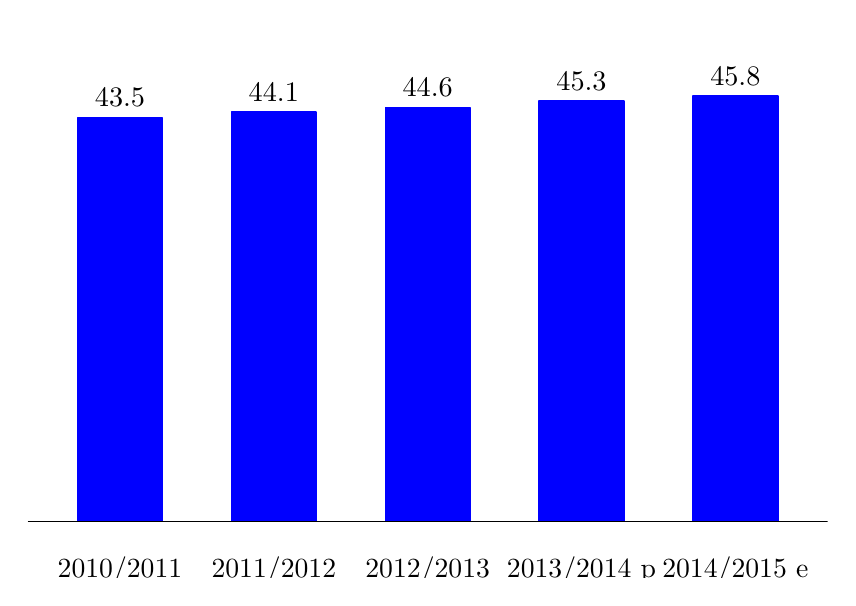
\begin{tikzpicture}[x=1pt,y=1pt]  % Created by tikzDevice version 0.9 on 2016-03-03 04:15:06
% !TEX encoding = UTF-8 Unicode
\definecolor{fillColor}{RGB}{255,255,255}
\path[use as bounding box,fill=fillColor,fill opacity=0.00] (0,0) rectangle (289.08,198.74);
\begin{scope}
\path[clip] (  0.00,  0.00) rectangle (289.08,198.74);

\path[] (  0.00,  0.00) rectangle (289.08,198.74);
\end{scope}
\begin{scope}
\path[clip] (  0.00,  0.00) rectangle (289.08,198.74);

\path[] (  0.00, 12.77) rectangle (289.08,181.67);

\path[] ( 33.36, 12.77) --
	( 33.36,181.67);

\path[] ( 88.95, 12.77) --
	( 88.95,181.67);

\path[] (144.54, 12.77) --
	(144.54,181.67);

\path[] (200.13, 12.77) --
	(200.13,181.67);

\path[] (255.72, 12.77) --
	(255.72,181.67);
\definecolor{drawColor}{RGB}{0,0,255}
\definecolor{fillColor}{RGB}{0,0,255}

\path[draw=drawColor,line width= 0.6pt,line join=round,fill=fillColor] ( 18.07, 20.44) rectangle ( 48.64,166.29);

\path[draw=drawColor,line width= 0.6pt,line join=round,fill=fillColor] ( 73.66, 20.44) rectangle (104.24,168.27);

\path[draw=drawColor,line width= 0.6pt,line join=round,fill=fillColor] (129.25, 20.44) rectangle (159.83,169.85);

\path[draw=drawColor,line width= 0.6pt,line join=round,fill=fillColor] (184.84, 20.44) rectangle (215.42,172.23);

\path[draw=drawColor,line width= 0.6pt,line join=round,fill=fillColor] (240.44, 20.44) rectangle (271.01,173.99);
\definecolor{drawColor}{RGB}{0,0,0}

\path[draw=drawColor,line width= 0.1pt,line join=round] (  0.00, 20.44) -- (289.08, 20.44);

\node[text=drawColor,anchor=base,inner sep=0pt, outer sep=0pt, scale=  1.02] at ( 33.36,170.26) {43.5};

\node[text=drawColor,anchor=base,inner sep=0pt, outer sep=0pt, scale=  1.02] at ( 88.95,172.24) {44.1};

\node[text=drawColor,anchor=base,inner sep=0pt, outer sep=0pt, scale=  1.02] at (144.54,173.83) {44.6};

\node[text=drawColor,anchor=base,inner sep=0pt, outer sep=0pt, scale=  1.02] at (200.13,176.20) {45.3};

\node[text=drawColor,anchor=base,inner sep=0pt, outer sep=0pt, scale=  1.02] at (255.72,177.96) {45.8};

\path[] (  0.00, 12.77) rectangle (289.08,181.67);
\end{scope}
\begin{scope}
\path[clip] (  0.00,  0.00) rectangle (289.08,198.74);

\path[] (  0.00, 12.77) --
	(289.08, 12.77);
\end{scope}
\begin{scope}
\path[clip] (  0.00,  0.00) rectangle (289.08,198.74);

\path[] ( 33.36, 10.02) --
	( 33.36, 12.77);

\path[] ( 88.95, 10.02) --
	( 88.95, 12.77);

\path[] (144.54, 10.02) --
	(144.54, 12.77);

\path[] (200.13, 10.02) --
	(200.13, 12.77);

\path[] (255.72, 10.02) --
	(255.72, 12.77);
\end{scope}
\begin{scope}
\path[clip] (  0.00,  0.00) rectangle (289.08,198.74);
\definecolor{drawColor}{RGB}{0,0,0}

\node[text=drawColor,anchor=base,inner sep=0pt, outer sep=0pt, scale=  1.00] at ( 33.36, -0.00) {2010/2011};

\node[text=drawColor,anchor=base,inner sep=0pt, outer sep=0pt, scale=  1.00] at ( 88.95, -0.00) {2011/2012};

\node[text=drawColor,anchor=base,inner sep=0pt, outer sep=0pt, scale=  1.00] at (144.54, -0.00) {2012/2013};

\node[text=drawColor,anchor=base,inner sep=0pt, outer sep=0pt, scale=  1.00] at (200.13, -0.00) {2013/2014 p};

\node[text=drawColor,anchor=base,inner sep=0pt, outer sep=0pt, scale=  1.00] at (255.72, -0.00) {2014/2015  e};
\end{scope}
  \end{tikzpicture}}%
{%
	Diplan-MAGA con datos de Banguat (MAGA, 2013).} %

%#########################7########################

\cajita{%
	Trigo }%
{%
}%
{%
	Área cosechada y producción de trigo} %
{%
	República de Guatemala, serie histórica, en manzanas y  quintales } %
{%
	\begin{tikzpicture}[x=1pt,y=1pt]  % Created by tikzDevice version 0.9 on 2016-03-03 04:15:07
% !TEX encoding = UTF-8 Unicode
\definecolor{fillColor}{RGB}{255,255,255}
\path[use as bounding box,fill=fillColor,fill opacity=0.00] (0,0) rectangle (289.08,198.74);
\begin{scope}
\path[clip] (  0.00,  0.00) rectangle (289.08,198.74);

\path[] (  0.00,  0.00) rectangle (289.08,198.74);
\end{scope}
\begin{scope}
\path[clip] (  0.00,  0.00) rectangle (289.08,198.74);

\path[] (  0.00, 18.46) rectangle (289.08,157.72);

\path[] ( 33.36, 18.46) --
	( 33.36,157.72);

\path[] ( 88.95, 18.46) --
	( 88.95,157.72);

\path[] (144.54, 18.46) --
	(144.54,157.72);

\path[] (200.13, 18.46) --
	(200.13,157.72);

\path[] (255.72, 18.46) --
	(255.72,157.72);
\definecolor{drawColor}{RGB}{0,0,255}
\definecolor{fillColor}{RGB}{0,0,255}

\path[draw=drawColor,line width= 0.6pt,line join=round,fill=fillColor] (  9.73, 18.46) rectangle ( 31.97, 22.22);
\definecolor{drawColor}{RGB}{157,187,255}
\definecolor{fillColor}{RGB}{157,187,255}

\path[draw=drawColor,line width= 0.6pt,line join=round,fill=fillColor] ( 34.75, 18.46) rectangle ( 56.98,141.70);
\definecolor{drawColor}{RGB}{0,0,255}
\definecolor{fillColor}{RGB}{0,0,255}

\path[draw=drawColor,line width= 0.6pt,line join=round,fill=fillColor] ( 65.32, 18.46) rectangle ( 87.56, 22.35);
\definecolor{drawColor}{RGB}{157,187,255}
\definecolor{fillColor}{RGB}{157,187,255}

\path[draw=drawColor,line width= 0.6pt,line join=round,fill=fillColor] ( 90.34, 18.46) rectangle (112.57,141.38);
\definecolor{drawColor}{RGB}{0,0,255}
\definecolor{fillColor}{RGB}{0,0,255}

\path[draw=drawColor,line width= 0.6pt,line join=round,fill=fillColor] (120.91, 18.46) rectangle (143.15, 22.35);
\definecolor{drawColor}{RGB}{157,187,255}
\definecolor{fillColor}{RGB}{157,187,255}

\path[draw=drawColor,line width= 0.6pt,line join=round,fill=fillColor] (145.93, 18.46) rectangle (168.17,148.39);
\definecolor{drawColor}{RGB}{0,0,255}
\definecolor{fillColor}{RGB}{0,0,255}

\path[draw=drawColor,line width= 0.6pt,line join=round,fill=fillColor] (176.51, 18.46) rectangle (198.74, 22.74);
\definecolor{drawColor}{RGB}{157,187,255}
\definecolor{fillColor}{RGB}{157,187,255}

\path[draw=drawColor,line width= 0.6pt,line join=round,fill=fillColor] (201.52, 18.46) rectangle (223.76,151.89);
\definecolor{drawColor}{RGB}{0,0,255}
\definecolor{fillColor}{RGB}{0,0,255}

\path[draw=drawColor,line width= 0.6pt,line join=round,fill=fillColor] (232.10, 18.46) rectangle (254.33, 22.74);
\definecolor{drawColor}{RGB}{157,187,255}
\definecolor{fillColor}{RGB}{157,187,255}

\path[draw=drawColor,line width= 0.6pt,line join=round,fill=fillColor] (257.11, 18.46) rectangle (279.35,157.72);
\definecolor{drawColor}{RGB}{0,0,0}

\path[draw=drawColor,line width= 0.6pt,line join=round] (  0.00, 18.46) -- (289.08, 18.46);

\node[text=drawColor,rotate= 90.00,anchor=base west,inner sep=0pt, outer sep=0pt, scale=  0.83] at ( 24.08, 24.40) {968};

\node[text=drawColor,rotate= 90.00,anchor=base west,inner sep=0pt, outer sep=0pt, scale=  0.83] at ( 49.10,145.70) {31,681};

\node[text=drawColor,rotate= 90.00,anchor=base west,inner sep=0pt, outer sep=0pt, scale=  0.83] at ( 79.67, 25.62) {1,000};

\node[text=drawColor,rotate= 90.00,anchor=base west,inner sep=0pt, outer sep=0pt, scale=  0.83] at (104.69,145.38) {31,600};

\node[text=drawColor,rotate= 90.00,anchor=base west,inner sep=0pt, outer sep=0pt, scale=  0.83] at (135.27, 25.62) {1,000};

\node[text=drawColor,rotate= 90.00,anchor=base west,inner sep=0pt, outer sep=0pt, scale=  0.83] at (160.28,152.38) {33,400};

\node[text=drawColor,rotate= 90.00,anchor=base west,inner sep=0pt, outer sep=0pt, scale=  0.83] at (190.86, 26.01) {1,100};

\node[text=drawColor,rotate= 90.00,anchor=base west,inner sep=0pt, outer sep=0pt, scale=  0.83] at (215.88,155.88) {34,300};

\node[text=drawColor,rotate= 90.00,anchor=base west,inner sep=0pt, outer sep=0pt, scale=  0.83] at (246.45, 26.01) {1,100};

\node[text=drawColor,rotate= 90.00,anchor=base west,inner sep=0pt, outer sep=0pt, scale=  0.83] at (271.47,161.72) {35,800};

\path[] (  0.00, 18.46) rectangle (289.08,157.72);
\end{scope}
\begin{scope}
\path[clip] (  0.00,  0.00) rectangle (289.08,198.74);

\path[] (  0.00, 18.46) --
	(289.08, 18.46);
\end{scope}
\begin{scope}
\path[clip] (  0.00,  0.00) rectangle (289.08,198.74);

\path[] ( 33.36, 15.71) --
	( 33.36, 18.46);

\path[] ( 88.95, 15.71) --
	( 88.95, 18.46);

\path[] (144.54, 15.71) --
	(144.54, 18.46);

\path[] (200.13, 15.71) --
	(200.13, 18.46);

\path[] (255.72, 15.71) --
	(255.72, 18.46);
\end{scope}
\begin{scope}
\path[clip] (  0.00,  0.00) rectangle (289.08,198.74);
\definecolor{drawColor}{RGB}{0,0,0}

\node[text=drawColor,anchor=base,inner sep=0pt, outer sep=0pt, scale=  1.00] at ( 33.36,  5.69) {2010/2011};

\node[text=drawColor,anchor=base,inner sep=0pt, outer sep=0pt, scale=  1.00] at ( 88.95,  5.69) {2011/2012};

\node[text=drawColor,anchor=base,inner sep=0pt, outer sep=0pt, scale=  1.00] at (144.54,  5.69) {2012/2013};

\node[text=drawColor,anchor=base,inner sep=0pt, outer sep=0pt, scale=  1.00] at (200.13,  5.69) {2013/2014 \llamada};

\node[text=drawColor,anchor=base,inner sep=0pt, outer sep=0pt, scale=  1.00] at (255.72,  5.69) {2014/2015  \llamada};
\end{scope}
\begin{scope}
\path[clip] (  0.00,  0.00) rectangle (289.08,198.74);
\coordinate (apoyo) at (61.96,191.07);
\coordinate (longitudFicticia) at (7.11,7.67);
\coordinate (longitud) at (7.11,7.11);
\coordinate (desX) at (128.08,0);
\coordinate (desY) at (0,0.28);
\definecolor[named]{ct1}{HTML}{
0000FF
}
\definecolor[named]{ct2}{HTML}{
9DBBFF
}
\definecolor[named]{ctb1}{HTML}{
0000FF
}
\definecolor[named]{ctb2}{HTML}{
9DBBFF
}
\path [fill=none] (apoyo) rectangle ($(apoyo)+(longitudFicticia)$)
node [xshift=0.3cm,inner sep=0pt, outer sep=0pt,midway,right,scale = 0.9]{Area};
\draw [color = ctb1,fill=ct1] ( $(apoyo)  + (desY) $) rectangle ($(apoyo)+ (desY) +(longitud)$);
\path [fill=none] ($(apoyo)+(desX)$) rectangle ($(apoyo)+(desX)+(longitudFicticia)$)
node [xshift=0.3cm,inner sep=0pt, outer sep=0pt,midway,right,scale = 0.9]{Producción};
\draw [color = ctb2 ,fill=ct2] ( $(apoyo)  + (desY) + (desX) $) rectangle ($(apoyo)+ (desY)+ (desX) +(longitud)$);
\end{scope}
  \end{tikzpicture}}%
{%
	MAGA} %


%#########################8########################

\cajita{%
	Rendimiento del trigo}%
{%
}%
{%
	Rendimiento del trigo} %
{%
	República de Guatemala, serie histórica, en quintales sobre manzanas } %
{%
	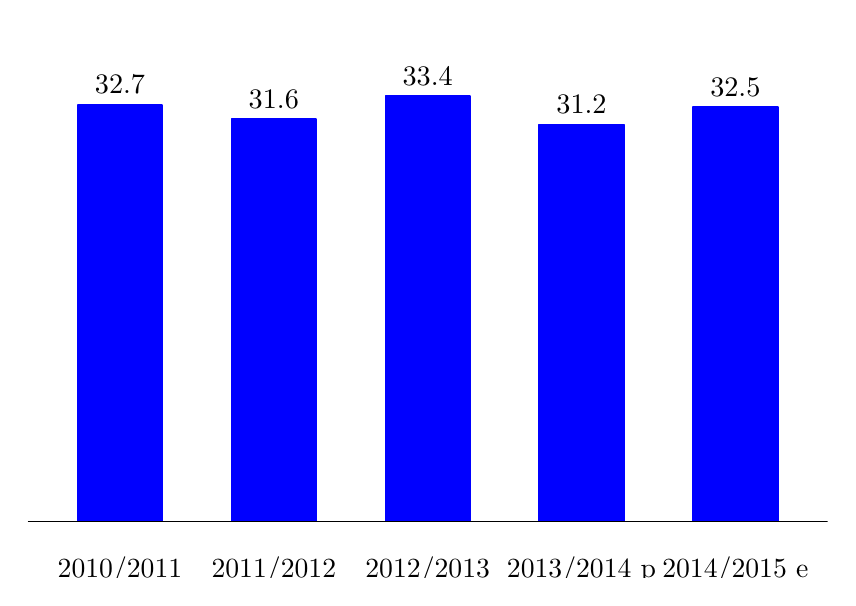
\begin{tikzpicture}[x=1pt,y=1pt]  % Created by tikzDevice version 0.9 on 2016-03-03 04:15:09
% !TEX encoding = UTF-8 Unicode
\definecolor{fillColor}{RGB}{255,255,255}
\path[use as bounding box,fill=fillColor,fill opacity=0.00] (0,0) rectangle (289.08,198.74);
\begin{scope}
\path[clip] (  0.00,  0.00) rectangle (289.08,198.74);

\path[] (  0.00,  0.00) rectangle (289.08,198.74);
\end{scope}
\begin{scope}
\path[clip] (  0.00,  0.00) rectangle (289.08,198.74);

\path[] (  0.00, 12.77) rectangle (289.08,181.67);

\path[] ( 33.36, 12.77) --
	( 33.36,181.67);

\path[] ( 88.95, 12.77) --
	( 88.95,181.67);

\path[] (144.54, 12.77) --
	(144.54,181.67);

\path[] (200.13, 12.77) --
	(200.13,181.67);

\path[] (255.72, 12.77) --
	(255.72,181.67);
\definecolor{drawColor}{RGB}{0,0,255}
\definecolor{fillColor}{RGB}{0,0,255}

\path[draw=drawColor,line width= 0.6pt,line join=round,fill=fillColor] ( 18.07, 20.44) rectangle ( 48.64,170.91);

\path[draw=drawColor,line width= 0.6pt,line join=round,fill=fillColor] ( 73.66, 20.44) rectangle (104.24,165.72);

\path[draw=drawColor,line width= 0.6pt,line join=round,fill=fillColor] (129.25, 20.44) rectangle (159.83,173.99);

\path[draw=drawColor,line width= 0.6pt,line join=round,fill=fillColor] (184.84, 20.44) rectangle (215.42,163.80);

\path[draw=drawColor,line width= 0.6pt,line join=round,fill=fillColor] (240.44, 20.44) rectangle (271.01,170.06);
\definecolor{drawColor}{RGB}{0,0,0}

\path[draw=drawColor,line width= 0.1pt,line join=round] (  0.00, 20.44) -- (289.08, 20.44);

\node[text=drawColor,anchor=base,inner sep=0pt, outer sep=0pt, scale=  1.02] at ( 33.36,174.88) {32.7};

\node[text=drawColor,anchor=base,inner sep=0pt, outer sep=0pt, scale=  1.02] at ( 88.95,169.69) {31.6};

\node[text=drawColor,anchor=base,inner sep=0pt, outer sep=0pt, scale=  1.02] at (144.54,177.96) {33.4};

\node[text=drawColor,anchor=base,inner sep=0pt, outer sep=0pt, scale=  1.02] at (200.13,167.77) {31.2};

\node[text=drawColor,anchor=base,inner sep=0pt, outer sep=0pt, scale=  1.02] at (255.72,174.04) {32.5};

\path[] (  0.00, 12.77) rectangle (289.08,181.67);
\end{scope}
\begin{scope}
\path[clip] (  0.00,  0.00) rectangle (289.08,198.74);

\path[] (  0.00, 12.77) --
	(289.08, 12.77);
\end{scope}
\begin{scope}
\path[clip] (  0.00,  0.00) rectangle (289.08,198.74);

\path[] ( 33.36, 10.02) --
	( 33.36, 12.77);

\path[] ( 88.95, 10.02) --
	( 88.95, 12.77);

\path[] (144.54, 10.02) --
	(144.54, 12.77);

\path[] (200.13, 10.02) --
	(200.13, 12.77);

\path[] (255.72, 10.02) --
	(255.72, 12.77);
\end{scope}
\begin{scope}
\path[clip] (  0.00,  0.00) rectangle (289.08,198.74);
\definecolor{drawColor}{RGB}{0,0,0}

\node[text=drawColor,anchor=base,inner sep=0pt, outer sep=0pt, scale=  1.00] at ( 33.36, -0.00) {2010/2011};

\node[text=drawColor,anchor=base,inner sep=0pt, outer sep=0pt, scale=  1.00] at ( 88.95, -0.00) {2011/2012};

\node[text=drawColor,anchor=base,inner sep=0pt, outer sep=0pt, scale=  1.00] at (144.54, -0.00) {2012/2013};

\node[text=drawColor,anchor=base,inner sep=0pt, outer sep=0pt, scale=  1.00] at (200.13, -0.00) {2013/2014 p};

\node[text=drawColor,anchor=base,inner sep=0pt, outer sep=0pt, scale=  1.00] at (255.72, -0.00) {2014/2015  e};
\end{scope}
  \end{tikzpicture}}%
{%
	MAGA } %

%#########################9########################

\cajita{%
	Ajonjolí }%
{%
}%
{%
	Área cosechada y producción de ajonjolí} %
{%
	República de Guatemala, serie histórica, en manzanas y  quintales } %
{%
	\begin{tikzpicture}[x=1pt,y=1pt]  % Created by tikzDevice version 0.9 on 2016-03-03 04:15:10
% !TEX encoding = UTF-8 Unicode
\definecolor{fillColor}{RGB}{255,255,255}
\path[use as bounding box,fill=fillColor,fill opacity=0.00] (0,0) rectangle (289.08,198.74);
\begin{scope}
\path[clip] (  0.00,  0.00) rectangle (289.08,198.74);

\path[] (  0.00,  0.00) rectangle (289.08,198.74);
\end{scope}
\begin{scope}
\path[clip] (  0.00,  0.00) rectangle (289.08,198.74);

\path[] (  0.00, 18.46) rectangle (289.08,146.67);

\path[] ( 33.36, 18.46) --
	( 33.36,146.67);

\path[] ( 88.95, 18.46) --
	( 88.95,146.67);

\path[] (144.54, 18.46) --
	(144.54,146.67);

\path[] (200.13, 18.46) --
	(200.13,146.67);

\path[] (255.72, 18.46) --
	(255.72,146.67);
\definecolor{drawColor}{RGB}{0,0,255}
\definecolor{fillColor}{RGB}{0,0,255}

\path[draw=drawColor,line width= 0.6pt,line join=round,fill=fillColor] (  9.73, 18.46) rectangle ( 31.97, 23.41);
\definecolor{drawColor}{RGB}{157,187,255}
\definecolor{fillColor}{RGB}{157,187,255}

\path[draw=drawColor,line width= 0.6pt,line join=round,fill=fillColor] ( 34.75, 18.46) rectangle ( 56.98,126.51);
\definecolor{drawColor}{RGB}{0,0,255}
\definecolor{fillColor}{RGB}{0,0,255}

\path[draw=drawColor,line width= 0.6pt,line join=round,fill=fillColor] ( 65.32, 18.46) rectangle ( 87.56, 22.70);
\definecolor{drawColor}{RGB}{157,187,255}
\definecolor{fillColor}{RGB}{157,187,255}

\path[draw=drawColor,line width= 0.6pt,line join=round,fill=fillColor] ( 90.34, 18.46) rectangle (112.57,103.97);
\definecolor{drawColor}{RGB}{0,0,255}
\definecolor{fillColor}{RGB}{0,0,255}

\path[draw=drawColor,line width= 0.6pt,line join=round,fill=fillColor] (120.91, 18.46) rectangle (143.15, 23.76);
\definecolor{drawColor}{RGB}{157,187,255}
\definecolor{fillColor}{RGB}{157,187,255}

\path[draw=drawColor,line width= 0.6pt,line join=round,fill=fillColor] (145.93, 18.46) rectangle (168.17,124.37);
\definecolor{drawColor}{RGB}{0,0,255}
\definecolor{fillColor}{RGB}{0,0,255}

\path[draw=drawColor,line width= 0.6pt,line join=round,fill=fillColor] (176.51, 18.46) rectangle (198.74, 23.98);
\definecolor{drawColor}{RGB}{157,187,255}
\definecolor{fillColor}{RGB}{157,187,255}

\path[draw=drawColor,line width= 0.6pt,line join=round,fill=fillColor] (201.52, 18.46) rectangle (223.76,146.67);
\definecolor{drawColor}{RGB}{0,0,255}
\definecolor{fillColor}{RGB}{0,0,255}

\path[draw=drawColor,line width= 0.6pt,line join=round,fill=fillColor] (232.10, 18.46) rectangle (254.33, 23.85);
\definecolor{drawColor}{RGB}{157,187,255}
\definecolor{fillColor}{RGB}{157,187,255}

\path[draw=drawColor,line width= 0.6pt,line join=round,fill=fillColor] (257.11, 18.46) rectangle (279.35,128.51);
\definecolor{drawColor}{RGB}{0,0,0}

\path[draw=drawColor,line width= 0.6pt,line join=round] (  0.00, 18.46) -- (289.08, 18.46);

\node[text=drawColor,rotate= 90.00,anchor=base west,inner sep=0pt, outer sep=0pt, scale=  0.83] at ( 24.08, 27.41) {50,378};

\node[text=drawColor,rotate= 90.00,anchor=base west,inner sep=0pt, outer sep=0pt, scale=  0.83] at ( 49.10,132.33) {1,099,422};

\node[text=drawColor,rotate= 90.00,anchor=base west,inner sep=0pt, outer sep=0pt, scale=  0.83] at ( 79.67, 26.70) {43,200};

\node[text=drawColor,rotate= 90.00,anchor=base west,inner sep=0pt, outer sep=0pt, scale=  0.83] at (104.69,108.70) {870,100};

\node[text=drawColor,rotate= 90.00,anchor=base west,inner sep=0pt, outer sep=0pt, scale=  0.83] at (135.27, 27.76) {54,000};

\node[text=drawColor,rotate= 90.00,anchor=base west,inner sep=0pt, outer sep=0pt, scale=  0.83] at (160.28,130.19) {1,077,600};

\node[text=drawColor,rotate= 90.00,anchor=base west,inner sep=0pt, outer sep=0pt, scale=  0.83] at (190.86, 27.98) {56,200};

\node[text=drawColor,rotate= 90.00,anchor=base west,inner sep=0pt, outer sep=0pt, scale=  0.83] at (215.88,152.49) {1,304,500};

\node[text=drawColor,rotate= 90.00,anchor=base west,inner sep=0pt, outer sep=0pt, scale=  0.83] at (246.45, 27.85) {54,900};

\node[text=drawColor,rotate= 90.00,anchor=base west,inner sep=0pt, outer sep=0pt, scale=  0.83] at (271.47,134.33) {1,119,800};

\path[] (  0.00, 18.46) rectangle (289.08,146.67);
\end{scope}
\begin{scope}
\path[clip] (  0.00,  0.00) rectangle (289.08,198.74);

\path[] (  0.00, 18.46) --
	(289.08, 18.46);
\end{scope}
\begin{scope}
\path[clip] (  0.00,  0.00) rectangle (289.08,198.74);

\path[] ( 33.36, 15.71) --
	( 33.36, 18.46);

\path[] ( 88.95, 15.71) --
	( 88.95, 18.46);

\path[] (144.54, 15.71) --
	(144.54, 18.46);

\path[] (200.13, 15.71) --
	(200.13, 18.46);

\path[] (255.72, 15.71) --
	(255.72, 18.46);
\end{scope}
\begin{scope}
\path[clip] (  0.00,  0.00) rectangle (289.08,198.74);
\definecolor{drawColor}{RGB}{0,0,0}

\node[text=drawColor,anchor=base,inner sep=0pt, outer sep=0pt, scale=  1.00] at ( 33.36,  5.69) {2010/2011};

\node[text=drawColor,anchor=base,inner sep=0pt, outer sep=0pt, scale=  1.00] at ( 88.95,  5.69) {2011/2012};

\node[text=drawColor,anchor=base,inner sep=0pt, outer sep=0pt, scale=  1.00] at (144.54,  5.69) {2012/2013};

<<<<<<< HEAD
\node[text=drawColor,anchor=base,inner sep=0pt, outer sep=0pt, scale=  1.00] at (200.13,  5.69) {2013/2014 \llamada};

\node[text=drawColor,anchor=base,inner sep=0pt, outer sep=0pt, scale=  1.00] at (255.72,  5.69) {2014/2015  \llamada};
=======
\node[text=drawColor,anchor=base,inner sep=0pt, outer sep=0pt, scale=  1.00] at (200.13,  5.69) {2013/2014 p};

\node[text=drawColor,anchor=base,inner sep=0pt, outer sep=0pt, scale=  1.00] at (255.72,  5.69) {2014/2015  e};
>>>>>>> origin/master
\end{scope}
\begin{scope}
\path[clip] (  0.00,  0.00) rectangle (289.08,198.74);
\coordinate (apoyo) at (61.96,191.07);
\coordinate (longitudFicticia) at (7.11,7.67);
\coordinate (longitud) at (7.11,7.11);
\coordinate (desX) at (128.08,0);
\coordinate (desY) at (0,0.28);
\definecolor[named]{ct1}{HTML}{
0000FF
}
\definecolor[named]{ct2}{HTML}{
9DBBFF
}
\definecolor[named]{ctb1}{HTML}{
0000FF
}
\definecolor[named]{ctb2}{HTML}{
9DBBFF
}
\path [fill=none] (apoyo) rectangle ($(apoyo)+(longitudFicticia)$)
node [xshift=0.3cm,inner sep=0pt, outer sep=0pt,midway,right,scale = 0.9]{Area};
\draw [color = ctb1,fill=ct1] ( $(apoyo)  + (desY) $) rectangle ($(apoyo)+ (desY) +(longitud)$);
\path [fill=none] ($(apoyo)+(desX)$) rectangle ($(apoyo)+(desX)+(longitudFicticia)$)
node [xshift=0.3cm,inner sep=0pt, outer sep=0pt,midway,right,scale = 0.9]{Producción};
\draw [color = ctb2 ,fill=ct2] ( $(apoyo)  + (desY) + (desX) $) rectangle ($(apoyo)+ (desY)+ (desX) +(longitud)$);
\end{scope}
  \end{tikzpicture}}%
{%
	Diplan-MAGA con datos de Banguat (MAGA, 2013).} %


%#########################10########################

\cajita{%
	Rendimiento del ajonjolí }%
{%
}%
{%
	Rendimiento del ajonjolí} %
{%
	República de Guatemala, serie histórica, en quintales sobre manzanas } %
{%
	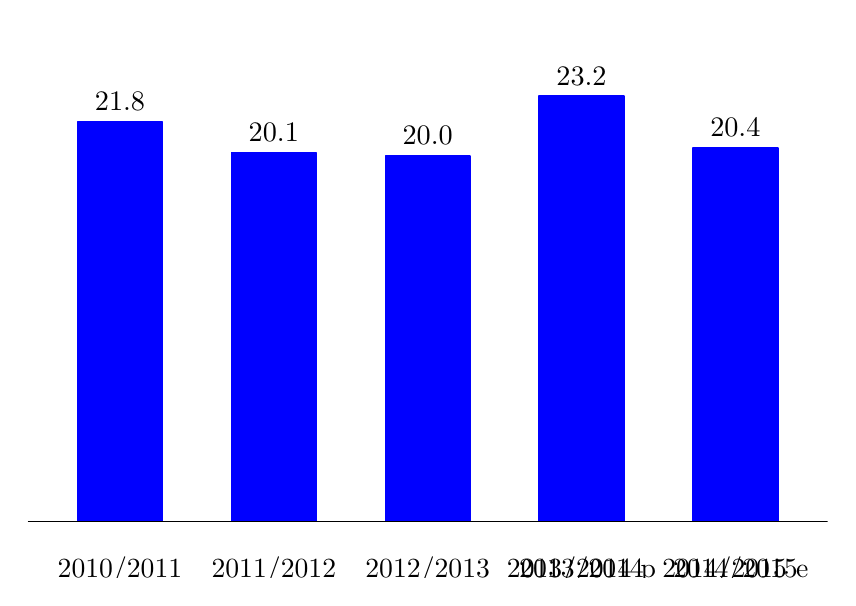
\begin{tikzpicture}[x=1pt,y=1pt]  % Created by tikzDevice version 0.9 on 2016-03-03 04:15:12
% !TEX encoding = UTF-8 Unicode
\definecolor{fillColor}{RGB}{255,255,255}
\path[use as bounding box,fill=fillColor,fill opacity=0.00] (0,0) rectangle (289.08,198.74);
\begin{scope}
\path[clip] (  0.00,  0.00) rectangle (289.08,198.74);

\path[] (  0.00,  0.00) rectangle (289.08,198.74);
\end{scope}
\begin{scope}
\path[clip] (  0.00,  0.00) rectangle (289.08,198.74);

\path[] (  0.00, 12.77) rectangle (289.08,181.67);

\path[] ( 33.36, 12.77) --
	( 33.36,181.67);

\path[] ( 88.95, 12.77) --
	( 88.95,181.67);

\path[] (144.54, 12.77) --
	(144.54,181.67);

\path[] (200.13, 12.77) --
	(200.13,181.67);

\path[] (255.72, 12.77) --
	(255.72,181.67);
\definecolor{drawColor}{RGB}{0,0,255}
\definecolor{fillColor}{RGB}{0,0,255}

\path[draw=drawColor,line width= 0.6pt,line join=round,fill=fillColor] ( 18.07, 20.44) rectangle ( 48.64,164.81);

\path[draw=drawColor,line width= 0.6pt,line join=round,fill=fillColor] ( 73.66, 20.44) rectangle (104.24,153.68);

\path[draw=drawColor,line width= 0.6pt,line join=round,fill=fillColor] (129.25, 20.44) rectangle (159.83,152.45);

\path[draw=drawColor,line width= 0.6pt,line join=round,fill=fillColor] (184.84, 20.44) rectangle (215.42,173.99);

\path[draw=drawColor,line width= 0.6pt,line join=round,fill=fillColor] (240.44, 20.44) rectangle (271.01,155.37);
\definecolor{drawColor}{RGB}{0,0,0}

\path[draw=drawColor,line width= 0.1pt,line join=round] (  0.00, 20.44) -- (289.08, 20.44);

\node[text=drawColor,anchor=base,inner sep=0pt, outer sep=0pt, scale=  1.02] at ( 33.36,168.78) {21.8};

\node[text=drawColor,anchor=base,inner sep=0pt, outer sep=0pt, scale=  1.02] at ( 88.95,157.65) {20.1};

\node[text=drawColor,anchor=base,inner sep=0pt, outer sep=0pt, scale=  1.02] at (144.54,156.42) {20.0};

\node[text=drawColor,anchor=base,inner sep=0pt, outer sep=0pt, scale=  1.02] at (200.13,177.96) {23.2};

\node[text=drawColor,anchor=base,inner sep=0pt, outer sep=0pt, scale=  1.02] at (255.72,159.34) {20.4};

\path[] (  0.00, 12.77) rectangle (289.08,181.67);
\end{scope}
\begin{scope}
\path[clip] (  0.00,  0.00) rectangle (289.08,198.74);

\path[] (  0.00, 12.77) --
	(289.08, 12.77);
\end{scope}
\begin{scope}
\path[clip] (  0.00,  0.00) rectangle (289.08,198.74);

\path[] ( 33.36, 10.02) --
	( 33.36, 12.77);

\path[] ( 88.95, 10.02) --
	( 88.95, 12.77);

\path[] (144.54, 10.02) --
	(144.54, 12.77);

\path[] (200.13, 10.02) --
	(200.13, 12.77);

\path[] (255.72, 10.02) --
	(255.72, 12.77);
\end{scope}
\begin{scope}
\path[clip] (  0.00,  0.00) rectangle (289.08,198.74);
\definecolor{drawColor}{RGB}{0,0,0}

\node[text=drawColor,anchor=base,inner sep=0pt, outer sep=0pt, scale=  1.00] at ( 33.36, -0.00) {2010/2011};

\node[text=drawColor,anchor=base,inner sep=0pt, outer sep=0pt, scale=  1.00] at ( 88.95, -0.00) {2011/2012};

\node[text=drawColor,anchor=base,inner sep=0pt, outer sep=0pt, scale=  1.00] at (144.54, -0.00) {2012/2013};

<<<<<<< HEAD
\node[text=drawColor,anchor=base,inner sep=0pt, outer sep=0pt, scale=  1.00] at (200.13, -0.00) {2013/2014 \llamada};

\node[text=drawColor,anchor=base,inner sep=0pt, outer sep=0pt, scale=  1.00] at (255.72, -0.00) {2014/2015  \llamada};
=======
\node[text=drawColor,anchor=base,inner sep=0pt, outer sep=0pt, scale=  1.00] at (200.13, -0.00) {2013/2014 p};

\node[text=drawColor,anchor=base,inner sep=0pt, outer sep=0pt, scale=  1.00] at (255.72, -0.00) {2014/2015  e};
>>>>>>> origin/master
\end{scope}
  \end{tikzpicture}}%
{%
	Diplan-MAGA con datos de Banguat (MAGA, 2013).} %


%#########################11########################

\cajita{%
	Balanza comercial de maíz blanco }%
{%
}%
{%
	Exportaciones, importaciones y balanza comercial de maíz blanco} %
{%
	República de Guatemala, serie histórica, en toneladas métricas } %
{%
	\begin{tikzpicture}[x=1pt,y=1pt]  % Created by tikzDevice version 0.9 on 2016-03-03 04:15:13
% !TEX encoding = UTF-8 Unicode
\definecolor{fillColor}{RGB}{255,255,255}
\path[use as bounding box,fill=fillColor,fill opacity=0.00] (0,0) rectangle (289.08,198.74);
\begin{scope}
\path[clip] (  0.00,  0.00) rectangle (289.08,198.74);

\path[] (  0.00,  0.00) rectangle (289.08,198.74);
\end{scope}
\begin{scope}
\path[clip] (  0.00,  0.00) rectangle (289.08,198.74);

\path[] (  0.00, 18.46) rectangle (289.08,148.78);

\path[] ( 33.36, 18.46) --
	( 33.36,148.78);

\path[] ( 88.95, 18.46) --
	( 88.95,148.78);

\path[] (144.54, 18.46) --
	(144.54,148.78);

\path[] (200.13, 18.46) --
	(200.13,148.78);

\path[] (255.72, 18.46) --
	(255.72,148.78);
\definecolor{drawColor}{RGB}{0,0,255}
\definecolor{fillColor}{RGB}{0,0,255}

\path[draw=drawColor,line width= 0.6pt,line join=round,fill=fillColor] (  9.27, 76.94) rectangle ( 24.09, 80.62);
\definecolor{drawColor}{RGB}{157,187,255}
\definecolor{fillColor}{RGB}{157,187,255}

\path[draw=drawColor,line width= 0.6pt,line join=round,fill=fillColor] ( 25.94, 76.94) rectangle ( 40.77,119.73);
\definecolor{drawColor}{RGB}{200,200,200}
\definecolor{fillColor}{RGB}{200,200,200}

\path[draw=drawColor,line width= 0.6pt,line join=round,fill=fillColor] ( 42.62, 37.84) rectangle ( 57.45, 76.94);
\definecolor{drawColor}{RGB}{0,0,255}
\definecolor{fillColor}{RGB}{0,0,255}

\path[draw=drawColor,line width= 0.6pt,line join=round,fill=fillColor] ( 64.86, 76.94) rectangle ( 79.68,101.43);
\definecolor{drawColor}{RGB}{157,187,255}
\definecolor{fillColor}{RGB}{157,187,255}

\path[draw=drawColor,line width= 0.6pt,line join=round,fill=fillColor] ( 81.54, 76.94) rectangle ( 96.36,148.78);
\definecolor{drawColor}{RGB}{200,200,200}
\definecolor{fillColor}{RGB}{200,200,200}

\path[draw=drawColor,line width= 0.6pt,line join=round,fill=fillColor] ( 98.21, 29.59) rectangle (113.04, 76.94);
\definecolor{drawColor}{RGB}{0,0,255}
\definecolor{fillColor}{RGB}{0,0,255}

\path[draw=drawColor,line width= 0.6pt,line join=round,fill=fillColor] (120.45, 76.94) rectangle (135.27, 81.38);
\definecolor{drawColor}{RGB}{157,187,255}
\definecolor{fillColor}{RGB}{157,187,255}

\path[draw=drawColor,line width= 0.6pt,line join=round,fill=fillColor] (137.13, 76.94) rectangle (151.95,139.87);
\definecolor{drawColor}{RGB}{200,200,200}
\definecolor{fillColor}{RGB}{200,200,200}

\path[draw=drawColor,line width= 0.6pt,line join=round,fill=fillColor] (153.81, 18.46) rectangle (168.63, 76.94);
\definecolor{drawColor}{RGB}{0,0,255}
\definecolor{fillColor}{RGB}{0,0,255}

\path[draw=drawColor,line width= 0.6pt,line join=round,fill=fillColor] (176.04, 76.94) rectangle (190.87, 91.15);
\definecolor{drawColor}{RGB}{157,187,255}
\definecolor{fillColor}{RGB}{157,187,255}

\path[draw=drawColor,line width= 0.6pt,line join=round,fill=fillColor] (192.72, 76.94) rectangle (207.54,108.80);
\definecolor{drawColor}{RGB}{200,200,200}
\definecolor{fillColor}{RGB}{200,200,200}

\path[draw=drawColor,line width= 0.6pt,line join=round,fill=fillColor] (209.40, 59.29) rectangle (224.22, 76.94);
\definecolor{drawColor}{RGB}{0,0,255}
\definecolor{fillColor}{RGB}{0,0,255}

\path[draw=drawColor,line width= 0.6pt,line join=round,fill=fillColor] (231.63, 76.94) rectangle (246.46, 80.39);
\definecolor{drawColor}{RGB}{157,187,255}
\definecolor{fillColor}{RGB}{157,187,255}

\path[draw=drawColor,line width= 0.6pt,line join=round,fill=fillColor] (248.31, 76.94) rectangle (263.14,116.85);
\definecolor{drawColor}{RGB}{200,200,200}
\definecolor{fillColor}{RGB}{200,200,200}

\path[draw=drawColor,line width= 0.6pt,line join=round,fill=fillColor] (264.99, 40.48) rectangle (279.81, 76.94);
\definecolor{drawColor}{RGB}{0,0,0}

\path[draw=drawColor,line width= 0.6pt,line join=round] (  0.00, 76.94) -- (289.08, 76.94);

\node[text=drawColor,rotate= 90.00,anchor=base west,inner sep=0pt, outer sep=0pt, scale=  0.83] at ( 19.91, 84.99) {2,127.5};

\node[text=drawColor,rotate= 90.00,anchor=base west,inner sep=0pt, outer sep=0pt, scale=  0.83] at ( 36.59,124.83) {24,745.3};

\node[text=drawColor,rotate= 90.00,anchor=base west,inner sep=0pt, outer sep=0pt, scale=  0.83] at ( 53.27, 43.39) {-22,617.8};

\node[text=drawColor,rotate= 90.00,anchor=base west,inner sep=0pt, outer sep=0pt, scale=  0.83] at ( 75.50,106.53) {14,164.0};

\node[text=drawColor,rotate= 90.00,anchor=base west,inner sep=0pt, outer sep=0pt, scale=  0.83] at ( 92.18,153.88) {41,547.8};

\node[text=drawColor,rotate= 90.00,anchor=base west,inner sep=0pt, outer sep=0pt, scale=  0.83] at (108.86, 35.15) {-27,383.8};

\node[text=drawColor,rotate= 90.00,anchor=base west,inner sep=0pt, outer sep=0pt, scale=  0.83] at (131.10, 85.76) {2,568.6};

\node[text=drawColor,rotate= 90.00,anchor=base west,inner sep=0pt, outer sep=0pt, scale=  0.83] at (147.77,144.97) {36,393.6};

\node[text=drawColor,rotate= 90.00,anchor=base west,inner sep=0pt, outer sep=0pt, scale=  0.83] at (164.45, 24.01) {-33,825.0};

\node[text=drawColor,rotate= 90.00,anchor=base west,inner sep=0pt, outer sep=0pt, scale=  0.83] at (186.69, 95.52) {8,214.9};

\node[text=drawColor,rotate= 90.00,anchor=base west,inner sep=0pt, outer sep=0pt, scale=  0.83] at (203.37,113.89) {18,422.1};

\node[text=drawColor,rotate= 90.00,anchor=base west,inner sep=0pt, outer sep=0pt, scale=  0.83] at (220.04, 24.85) {-10,207.1};

\node[text=drawColor,rotate= 90.00,anchor=base west,inner sep=0pt, outer sep=0pt, scale=  0.83] at (242.28, 84.76) {1,995.0};

\node[text=drawColor,rotate= 90.00,anchor=base west,inner sep=0pt, outer sep=0pt, scale=  0.83] at (258.96,121.95) {23,081.3};

\node[text=drawColor,rotate= 90.00,anchor=base west,inner sep=0pt, outer sep=0pt, scale=  0.83] at (275.64, 46.04) {-21,086.3};

\path[] (  0.00, 18.46) rectangle (289.08,148.78);
\end{scope}
\begin{scope}
\path[clip] (  0.00,  0.00) rectangle (289.08,198.74);

\path[] (  0.00, 18.46) --
	(289.08, 18.46);
\end{scope}
\begin{scope}
\path[clip] (  0.00,  0.00) rectangle (289.08,198.74);

\path[] ( 33.36, 15.71) --
	( 33.36, 18.46);

\path[] ( 88.95, 15.71) --
	( 88.95, 18.46);

\path[] (144.54, 15.71) --
	(144.54, 18.46);

\path[] (200.13, 15.71) --
	(200.13, 18.46);

\path[] (255.72, 15.71) --
	(255.72, 18.46);
\end{scope}
\begin{scope}
\path[clip] (  0.00,  0.00) rectangle (289.08,198.74);
\definecolor{drawColor}{RGB}{0,0,0}

\node[text=drawColor,anchor=base,inner sep=0pt, outer sep=0pt, scale=  1.00] at ( 33.36,  5.69) {2010};

\node[text=drawColor,anchor=base,inner sep=0pt, outer sep=0pt, scale=  1.00] at ( 88.95,  5.69) {2011};

\node[text=drawColor,anchor=base,inner sep=0pt, outer sep=0pt, scale=  1.00] at (144.54,  5.69) {2012};

\node[text=drawColor,anchor=base,inner sep=0pt, outer sep=0pt, scale=  1.00] at (200.13,  5.69) {2013};

\node[text=drawColor,anchor=base,inner sep=0pt, outer sep=0pt, scale=  1.00] at (255.72,  5.69) {2014*};
\end{scope}
\begin{scope}
\path[clip] (  0.00,  0.00) rectangle (289.08,198.74);
\coordinate (apoyo1) at (25.51,188.79);
\coordinate (apoyo2) at (117.41,188.79);
\coordinate (apoyo3) at (217.03,188.79);
\coordinate (longitudFicticia) at (7.11,9.95);
\coordinate (longitud) at (7.11,7.11);
\coordinate (desY) at (0,1.42);
\definecolor[named]{ct1}{HTML}{
0000FF
}
\definecolor[named]{ct2}{HTML}{
9DBBFF
}
\definecolor[named]{ct3}{HTML}{
C8C8C8
}
\definecolor[named]{ctb1}{HTML}{
0000FF
}
\definecolor[named]{ctb2}{HTML}{
9DBBFF
}
\definecolor[named]{ctb3}{HTML}{
C8C8C8
}
\path [fill=none] (apoyo1) rectangle ($(apoyo1)+(longitudFicticia)$)
node [xshift=0.3cm,inner sep=0pt, outer sep=0pt,text width=1.33333333333333in,midway,right,scale = 0.9]{Exportación};
\draw [color= ctb1, fill=ct1] ( $(apoyo1)  + (desY) $) rectangle ($(apoyo1)+ (desY) +(longitud)$);
\path [fill=none] (apoyo2) rectangle ($(apoyo2)+(longitudFicticia)$)
node [xshift=0.3cm,inner sep=0pt, outer sep=0pt,text width=1.33333333333333in,midway,right,scale = 0.9]{Importación};
\draw [color = ctb2, fill=ct2] ( $(apoyo2)  + (desY) $) rectangle ($(apoyo2)+ (desY) +(longitud)$);
\path [fill=none] (apoyo3) rectangle ($(apoyo3)+(longitudFicticia)$)
node [xshift=0.3cm,inner sep=0pt, outer sep=0pt,text width=1.33333333333333in,midway,right,scale = 0.9]{Balanza};
\path [color = ctb3, fill=ct3] ( $(apoyo3)  + (desY) $) rectangle ($(apoyo3)+ (desY) +(longitud)$);
\end{scope}
  \end{tikzpicture}}%
{%
	Diplan-MAGA con datos de Banguat (MAGA, 2013).} %


%#########################12########################

\cajita{%
	Balanza comercial de maíz amarillo }%
{%
}%
{%
	Exportaciones, importaciones y balanza comercial de maíz amarillo} %
{%
	República de Guatemala, serie histórica, en toneladas métricas } %
{%
	\begin{tikzpicture}[x=1pt,y=1pt]  % Created by tikzDevice version 0.9 on 2016-03-03 04:15:16
% !TEX encoding = UTF-8 Unicode
\definecolor{fillColor}{RGB}{255,255,255}
\path[use as bounding box,fill=fillColor,fill opacity=0.00] (0,0) rectangle (289.08,198.74);
\begin{scope}
\path[clip] (  0.00,  0.00) rectangle (289.08,198.74);

\path[] (  0.00,  0.00) rectangle (289.08,198.74);
\end{scope}
\begin{scope}
\path[clip] (  0.00,  0.00) rectangle (289.08,198.74);

\path[] (  0.00, 18.46) rectangle (289.08,144.39);

\path[] ( 33.36, 18.46) --
	( 33.36,144.39);

\path[] ( 88.95, 18.46) --
	( 88.95,144.39);

\path[] (144.54, 18.46) --
	(144.54,144.39);

\path[] (200.13, 18.46) --
	(200.13,144.39);

\path[] (255.72, 18.46) --
	(255.72,144.39);
\definecolor{drawColor}{RGB}{0,0,255}
\definecolor{fillColor}{RGB}{0,0,255}

\path[draw=drawColor,line width= 0.6pt,line join=round,fill=fillColor] (  9.27, 81.42) rectangle ( 24.09, 81.50);
\definecolor{drawColor}{RGB}{157,187,255}
\definecolor{fillColor}{RGB}{157,187,255}

\path[draw=drawColor,line width= 0.6pt,line join=round,fill=fillColor] ( 25.94, 81.42) rectangle ( 40.77,138.22);
\definecolor{drawColor}{RGB}{200,200,200}
\definecolor{fillColor}{RGB}{200,200,200}

\path[draw=drawColor,line width= 0.6pt,line join=round,fill=fillColor] ( 42.62, 24.69) rectangle ( 57.45, 81.42);
\definecolor{drawColor}{RGB}{0,0,255}
\definecolor{fillColor}{RGB}{0,0,255}

\path[draw=drawColor,line width= 0.6pt,line join=round,fill=fillColor] ( 64.86, 81.42) rectangle ( 79.68, 81.42);
\definecolor{drawColor}{RGB}{157,187,255}
\definecolor{fillColor}{RGB}{157,187,255}

\path[draw=drawColor,line width= 0.6pt,line join=round,fill=fillColor] ( 81.54, 81.42) rectangle ( 96.36,144.31);
\definecolor{drawColor}{RGB}{200,200,200}
\definecolor{fillColor}{RGB}{200,200,200}

\path[draw=drawColor,line width= 0.6pt,line join=round,fill=fillColor] ( 98.21, 18.53) rectangle (113.04, 81.42);
\definecolor{drawColor}{RGB}{0,0,255}
\definecolor{fillColor}{RGB}{0,0,255}

\path[draw=drawColor,line width= 0.6pt,line join=round,fill=fillColor] (120.45, 81.42) rectangle (135.27, 81.42);
\definecolor{drawColor}{RGB}{157,187,255}
\definecolor{fillColor}{RGB}{157,187,255}

\path[draw=drawColor,line width= 0.6pt,line join=round,fill=fillColor] (137.13, 81.42) rectangle (151.95,142.98);
\definecolor{drawColor}{RGB}{200,200,200}
\definecolor{fillColor}{RGB}{200,200,200}

\path[draw=drawColor,line width= 0.6pt,line join=round,fill=fillColor] (153.81, 19.86) rectangle (168.63, 81.42);
\definecolor{drawColor}{RGB}{0,0,255}
\definecolor{fillColor}{RGB}{0,0,255}

\path[draw=drawColor,line width= 0.6pt,line join=round,fill=fillColor] (176.04, 81.42) rectangle (190.87, 81.42);
\definecolor{drawColor}{RGB}{157,187,255}
\definecolor{fillColor}{RGB}{157,187,255}

\path[draw=drawColor,line width= 0.6pt,line join=round,fill=fillColor] (192.72, 81.42) rectangle (207.54,144.39);
\definecolor{drawColor}{RGB}{200,200,200}
\definecolor{fillColor}{RGB}{200,200,200}

\path[draw=drawColor,line width= 0.6pt,line join=round,fill=fillColor] (209.40, 18.46) rectangle (224.22, 81.42);
\definecolor{drawColor}{RGB}{0,0,255}
\definecolor{fillColor}{RGB}{0,0,255}

\path[draw=drawColor,line width= 0.6pt,line join=round,fill=fillColor] (231.63, 81.42) rectangle (246.46, 81.42);
\definecolor{drawColor}{RGB}{157,187,255}
\definecolor{fillColor}{RGB}{157,187,255}

\path[draw=drawColor,line width= 0.6pt,line join=round,fill=fillColor] (248.31, 81.42) rectangle (263.14,130.43);
\definecolor{drawColor}{RGB}{200,200,200}
\definecolor{fillColor}{RGB}{200,200,200}

\path[draw=drawColor,line width= 0.6pt,line join=round,fill=fillColor] (264.99, 32.42) rectangle (279.81, 81.42);
\definecolor{drawColor}{RGB}{0,0,0}

\path[draw=drawColor,line width= 0.6pt,line join=round] (  0.00, 81.42) -- (289.08, 81.42);

\node[text=drawColor,rotate= 90.00,anchor=base west,inner sep=0pt, outer sep=0pt, scale=  0.83] at ( 19.91, 84.77) {782.3};

\node[text=drawColor,rotate= 90.00,anchor=base west,inner sep=0pt, outer sep=0pt, scale=  0.83] at ( 36.59,144.04) {602,003.1};

\node[text=drawColor,rotate= 90.00,anchor=base west,inner sep=0pt, outer sep=0pt, scale=  0.83] at ( 53.27, 30.97) {-601,220.8};

\node[text=drawColor,rotate= 90.00,anchor=base west,inner sep=0pt, outer sep=0pt, scale=  0.83] at ( 75.50, 83.24) {0.0};

\node[text=drawColor,rotate= 90.00,anchor=base west,inner sep=0pt, outer sep=0pt, scale=  0.83] at ( 92.18,150.13) {666,495.0};

\node[text=drawColor,rotate= 90.00,anchor=base west,inner sep=0pt, outer sep=0pt, scale=  0.83] at (108.86, 24.81) {-666,495.0};

\node[text=drawColor,rotate= 90.00,anchor=base west,inner sep=0pt, outer sep=0pt, scale=  0.83] at (131.10, 83.25) {2.5};

\node[text=drawColor,rotate= 90.00,anchor=base west,inner sep=0pt, outer sep=0pt, scale=  0.83] at (147.77,148.81) {652,455.8};

\node[text=drawColor,rotate= 90.00,anchor=base west,inner sep=0pt, outer sep=0pt, scale=  0.83] at (164.45, 26.14) {-652,453.3};

\node[text=drawColor,rotate= 90.00,anchor=base west,inner sep=0pt, outer sep=0pt, scale=  0.83] at (186.69, 83.25) {4.1};

\node[text=drawColor,rotate= 90.00,anchor=base west,inner sep=0pt, outer sep=0pt, scale=  0.83] at (203.37,150.21) {667,311.8};

\node[text=drawColor,rotate= 90.00,anchor=base west,inner sep=0pt, outer sep=0pt, scale=  0.83] at (220.04, 24.74) {-667,307.8};

\node[text=drawColor,rotate= 90.00,anchor=base west,inner sep=0pt, outer sep=0pt, scale=  0.83] at (242.28, 83.97) {25.2};

\node[text=drawColor,rotate= 90.00,anchor=base west,inner sep=0pt, outer sep=0pt, scale=  0.83] at (258.96,136.25) {519,406.2};

\node[text=drawColor,rotate= 90.00,anchor=base west,inner sep=0pt, outer sep=0pt, scale=  0.83] at (275.64, 38.69) {-519,381.0};

\path[] (  0.00, 18.46) rectangle (289.08,144.39);
\end{scope}
\begin{scope}
\path[clip] (  0.00,  0.00) rectangle (289.08,198.74);

\path[] (  0.00, 18.46) --
	(289.08, 18.46);
\end{scope}
\begin{scope}
\path[clip] (  0.00,  0.00) rectangle (289.08,198.74);

\path[] ( 33.36, 15.71) --
	( 33.36, 18.46);

\path[] ( 88.95, 15.71) --
	( 88.95, 18.46);

\path[] (144.54, 15.71) --
	(144.54, 18.46);

\path[] (200.13, 15.71) --
	(200.13, 18.46);

\path[] (255.72, 15.71) --
	(255.72, 18.46);
\end{scope}
\begin{scope}
\path[clip] (  0.00,  0.00) rectangle (289.08,198.74);
\definecolor{drawColor}{RGB}{0,0,0}

\node[text=drawColor,anchor=base,inner sep=0pt, outer sep=0pt, scale=  1.00] at ( 33.36,  5.69) {2010};

\node[text=drawColor,anchor=base,inner sep=0pt, outer sep=0pt, scale=  1.00] at ( 88.95,  5.69) {2011};

\node[text=drawColor,anchor=base,inner sep=0pt, outer sep=0pt, scale=  1.00] at (144.54,  5.69) {2012};

\node[text=drawColor,anchor=base,inner sep=0pt, outer sep=0pt, scale=  1.00] at (200.13,  5.69) {2013};

\node[text=drawColor,anchor=base,inner sep=0pt, outer sep=0pt, scale=  1.00] at (255.72,  5.69) {2014*};
\end{scope}
\begin{scope}
\path[clip] (  0.00,  0.00) rectangle (289.08,198.74);
\coordinate (apoyo1) at (25.51,188.79);
\coordinate (apoyo2) at (117.41,188.79);
\coordinate (apoyo3) at (217.03,188.79);
\coordinate (longitudFicticia) at (7.11,9.95);
\coordinate (longitud) at (7.11,7.11);
\coordinate (desY) at (0,1.42);
\definecolor[named]{ct1}{HTML}{
0000FF
}
\definecolor[named]{ct2}{HTML}{
9DBBFF
}
\definecolor[named]{ct3}{HTML}{
C8C8C8
}
\definecolor[named]{ctb1}{HTML}{
0000FF
}
\definecolor[named]{ctb2}{HTML}{
9DBBFF
}
\definecolor[named]{ctb3}{HTML}{
C8C8C8
}
\path [fill=none] (apoyo1) rectangle ($(apoyo1)+(longitudFicticia)$)
node [xshift=0.3cm,inner sep=0pt, outer sep=0pt,text width=1.33333333333333in,midway,right,scale = 0.9]{Exportación};
\draw [color= ctb1, fill=ct1] ( $(apoyo1)  + (desY) $) rectangle ($(apoyo1)+ (desY) +(longitud)$);
\path [fill=none] (apoyo2) rectangle ($(apoyo2)+(longitudFicticia)$)
node [xshift=0.3cm,inner sep=0pt, outer sep=0pt,text width=1.33333333333333in,midway,right,scale = 0.9]{Importación};
\draw [color = ctb2, fill=ct2] ( $(apoyo2)  + (desY) $) rectangle ($(apoyo2)+ (desY) +(longitud)$);
\path [fill=none] (apoyo3) rectangle ($(apoyo3)+(longitudFicticia)$)
node [xshift=0.3cm,inner sep=0pt, outer sep=0pt,text width=1.33333333333333in,midway,right,scale = 0.9]{Balanza};
\path [color = ctb3, fill=ct3] ( $(apoyo3)  + (desY) $) rectangle ($(apoyo3)+ (desY) +(longitud)$);
\end{scope}
  \end{tikzpicture}}%
{%
	Diplan-MAGA con datos de Banguat (MAGA, 2013).} %



%#########################13########################

\cajita{%
	Balanza comercial del frijol }%
{%
}%
{%
	Exportaciones, importaciones y balanza comercial del frijol} %
{%
	República de Guatemala, serie histórica, en toneladas métricas } %
{%
	\begin{tikzpicture}[x=1pt,y=1pt]  % Created by tikzDevice version 0.9 on 2016-03-03 04:15:19
% !TEX encoding = UTF-8 Unicode
\definecolor{fillColor}{RGB}{255,255,255}
\path[use as bounding box,fill=fillColor,fill opacity=0.00] (0,0) rectangle (289.08,198.74);
\begin{scope}
\path[clip] (  0.00,  0.00) rectangle (289.08,198.74);

\path[] (  0.00,  0.00) rectangle (289.08,198.74);
\end{scope}
\begin{scope}
\path[clip] (  0.00,  0.00) rectangle (289.08,198.74);

\path[] (  0.00, 18.46) rectangle (289.08,148.78);

\path[] ( 33.36, 18.46) --
	( 33.36,148.78);

\path[] ( 88.95, 18.46) --
	( 88.95,148.78);

\path[] (144.54, 18.46) --
	(144.54,148.78);

\path[] (200.13, 18.46) --
	(200.13,148.78);

\path[] (255.72, 18.46) --
	(255.72,148.78);
\definecolor{drawColor}{RGB}{0,0,255}
\definecolor{fillColor}{RGB}{0,0,255}

\path[draw=drawColor,line width= 0.6pt,line join=round,fill=fillColor] (  9.27, 81.03) rectangle ( 24.09, 85.14);
\definecolor{drawColor}{RGB}{157,187,255}
\definecolor{fillColor}{RGB}{157,187,255}

\path[draw=drawColor,line width= 0.6pt,line join=round,fill=fillColor] ( 25.94, 81.03) rectangle ( 40.77,120.35);
\definecolor{drawColor}{RGB}{200,200,200}
\definecolor{fillColor}{RGB}{200,200,200}

\path[draw=drawColor,line width= 0.6pt,line join=round,fill=fillColor] ( 42.62, 45.83) rectangle ( 57.45, 81.03);
\definecolor{drawColor}{RGB}{0,0,255}
\definecolor{fillColor}{RGB}{0,0,255}

\path[draw=drawColor,line width= 0.6pt,line join=round,fill=fillColor] ( 64.86, 81.03) rectangle ( 79.68, 86.21);
\definecolor{drawColor}{RGB}{157,187,255}
\definecolor{fillColor}{RGB}{157,187,255}

\path[draw=drawColor,line width= 0.6pt,line join=round,fill=fillColor] ( 81.54, 81.03) rectangle ( 96.36,148.78);
\definecolor{drawColor}{RGB}{200,200,200}
\definecolor{fillColor}{RGB}{200,200,200}

\path[draw=drawColor,line width= 0.6pt,line join=round,fill=fillColor] ( 98.21, 18.46) rectangle (113.04, 81.03);
\definecolor{drawColor}{RGB}{0,0,255}
\definecolor{fillColor}{RGB}{0,0,255}

\path[draw=drawColor,line width= 0.6pt,line join=round,fill=fillColor] (120.45, 81.03) rectangle (135.27, 81.75);
\definecolor{drawColor}{RGB}{157,187,255}
\definecolor{fillColor}{RGB}{157,187,255}

\path[draw=drawColor,line width= 0.6pt,line join=round,fill=fillColor] (137.13, 81.03) rectangle (151.95,117.26);
\definecolor{drawColor}{RGB}{200,200,200}
\definecolor{fillColor}{RGB}{200,200,200}

\path[draw=drawColor,line width= 0.6pt,line join=round,fill=fillColor] (153.81, 45.52) rectangle (168.63, 81.03);
\definecolor{drawColor}{RGB}{0,0,255}
\definecolor{fillColor}{RGB}{0,0,255}

\path[draw=drawColor,line width= 0.6pt,line join=round,fill=fillColor] (176.04, 81.03) rectangle (190.87, 86.01);
\definecolor{drawColor}{RGB}{157,187,255}
\definecolor{fillColor}{RGB}{157,187,255}

\path[draw=drawColor,line width= 0.6pt,line join=round,fill=fillColor] (192.72, 81.03) rectangle (207.54,102.20);
\definecolor{drawColor}{RGB}{200,200,200}
\definecolor{fillColor}{RGB}{200,200,200}

\path[draw=drawColor,line width= 0.6pt,line join=round,fill=fillColor] (209.40, 64.84) rectangle (224.22, 81.03);
\definecolor{drawColor}{RGB}{0,0,255}
\definecolor{fillColor}{RGB}{0,0,255}

\path[draw=drawColor,line width= 0.6pt,line join=round,fill=fillColor] (231.63, 81.03) rectangle (246.46, 88.37);
\definecolor{drawColor}{RGB}{157,187,255}
\definecolor{fillColor}{RGB}{157,187,255}

\path[draw=drawColor,line width= 0.6pt,line join=round,fill=fillColor] (248.31, 81.03) rectangle (263.14, 93.70);
\definecolor{drawColor}{RGB}{200,200,200}
\definecolor{fillColor}{RGB}{200,200,200}

\path[draw=drawColor,line width= 0.6pt,line join=round,fill=fillColor] (264.99, 75.70) rectangle (279.81, 81.03);
\definecolor{drawColor}{RGB}{0,0,0}

\path[draw=drawColor,line width= 0.6pt,line join=round] (  0.00, 81.03) -- (289.08, 81.03);

\node[text=drawColor,rotate= 90.00,anchor=base west,inner sep=0pt, outer sep=0pt, scale=  0.83] at ( 19.91, 89.52) {1,246.3};

\node[text=drawColor,rotate= 90.00,anchor=base west,inner sep=0pt, outer sep=0pt, scale=  0.83] at ( 36.59,125.44) {11,913.9};

\node[text=drawColor,rotate= 90.00,anchor=base west,inner sep=0pt, outer sep=0pt, scale=  0.83] at ( 53.27, 51.38) {-10,667.6};

\node[text=drawColor,rotate= 90.00,anchor=base west,inner sep=0pt, outer sep=0pt, scale=  0.83] at ( 75.50, 90.58) {1,568.0};

\node[text=drawColor,rotate= 90.00,anchor=base west,inner sep=0pt, outer sep=0pt, scale=  0.83] at ( 92.18,153.88) {20,531.0};

\node[text=drawColor,rotate= 90.00,anchor=base west,inner sep=0pt, outer sep=0pt, scale=  0.83] at (108.86, 24.01) {-18,963.0};

\node[text=drawColor,rotate= 90.00,anchor=base west,inner sep=0pt, outer sep=0pt, scale=  0.83] at (131.10, 85.02) {216.9};

\node[text=drawColor,rotate= 90.00,anchor=base west,inner sep=0pt, outer sep=0pt, scale=  0.83] at (147.77,122.36) {10,980.1};

\node[text=drawColor,rotate= 90.00,anchor=base west,inner sep=0pt, outer sep=0pt, scale=  0.83] at (164.45, 51.07) {-10,763.2};

\node[text=drawColor,rotate= 90.00,anchor=base west,inner sep=0pt, outer sep=0pt, scale=  0.83] at (186.69, 90.38) {1,508.0};

\node[text=drawColor,rotate= 90.00,anchor=base west,inner sep=0pt, outer sep=0pt, scale=  0.83] at (203.37,106.57) {6,414.1};

\node[text=drawColor,rotate= 90.00,anchor=base west,inner sep=0pt, outer sep=0pt, scale=  0.83] at (220.04, 69.67) {-4,906.1};

\node[text=drawColor,rotate= 90.00,anchor=base west,inner sep=0pt, outer sep=0pt, scale=  0.83] at (242.28, 92.74) {2,222.7};

\node[text=drawColor,rotate= 90.00,anchor=base west,inner sep=0pt, outer sep=0pt, scale=  0.83] at (258.96, 98.07) {3,839.2};

\node[text=drawColor,rotate= 90.00,anchor=base west,inner sep=0pt, outer sep=0pt, scale=  0.83] at (275.64, 80.53) {-1,616.5};

\path[] (  0.00, 18.46) rectangle (289.08,148.78);
\end{scope}
\begin{scope}
\path[clip] (  0.00,  0.00) rectangle (289.08,198.74);

\path[] (  0.00, 18.46) --
	(289.08, 18.46);
\end{scope}
\begin{scope}
\path[clip] (  0.00,  0.00) rectangle (289.08,198.74);

\path[] ( 33.36, 15.71) --
	( 33.36, 18.46);

\path[] ( 88.95, 15.71) --
	( 88.95, 18.46);

\path[] (144.54, 15.71) --
	(144.54, 18.46);

\path[] (200.13, 15.71) --
	(200.13, 18.46);

\path[] (255.72, 15.71) --
	(255.72, 18.46);
\end{scope}
\begin{scope}
\path[clip] (  0.00,  0.00) rectangle (289.08,198.74);
\definecolor{drawColor}{RGB}{0,0,0}

\node[text=drawColor,anchor=base,inner sep=0pt, outer sep=0pt, scale=  1.00] at ( 33.36,  5.69) {2010};

\node[text=drawColor,anchor=base,inner sep=0pt, outer sep=0pt, scale=  1.00] at ( 88.95,  5.69) {2011};

\node[text=drawColor,anchor=base,inner sep=0pt, outer sep=0pt, scale=  1.00] at (144.54,  5.69) {2012};

\node[text=drawColor,anchor=base,inner sep=0pt, outer sep=0pt, scale=  1.00] at (200.13,  5.69) {2013};

\node[text=drawColor,anchor=base,inner sep=0pt, outer sep=0pt, scale=  1.00] at (255.72,  5.69) {2014*};
\end{scope}
\begin{scope}
\path[clip] (  0.00,  0.00) rectangle (289.08,198.74);
\coordinate (apoyo1) at (25.51,188.79);
\coordinate (apoyo2) at (117.41,188.79);
\coordinate (apoyo3) at (217.03,188.79);
\coordinate (longitudFicticia) at (7.11,9.95);
\coordinate (longitud) at (7.11,7.11);
\coordinate (desY) at (0,1.42);
\definecolor[named]{ct1}{HTML}{
0000FF
}
\definecolor[named]{ct2}{HTML}{
9DBBFF
}
\definecolor[named]{ct3}{HTML}{
C8C8C8
}
\definecolor[named]{ctb1}{HTML}{
0000FF
}
\definecolor[named]{ctb2}{HTML}{
9DBBFF
}
\definecolor[named]{ctb3}{HTML}{
C8C8C8
}
\path [fill=none] (apoyo1) rectangle ($(apoyo1)+(longitudFicticia)$)
node [xshift=0.3cm,inner sep=0pt, outer sep=0pt,text width=1.33333333333333in,midway,right,scale = 0.9]{Exportación};
\draw [color= ctb1, fill=ct1] ( $(apoyo1)  + (desY) $) rectangle ($(apoyo1)+ (desY) +(longitud)$);
\path [fill=none] (apoyo2) rectangle ($(apoyo2)+(longitudFicticia)$)
node [xshift=0.3cm,inner sep=0pt, outer sep=0pt,text width=1.33333333333333in,midway,right,scale = 0.9]{Importación};
\draw [color = ctb2, fill=ct2] ( $(apoyo2)  + (desY) $) rectangle ($(apoyo2)+ (desY) +(longitud)$);
\path [fill=none] (apoyo3) rectangle ($(apoyo3)+(longitudFicticia)$)
node [xshift=0.3cm,inner sep=0pt, outer sep=0pt,text width=1.33333333333333in,midway,right,scale = 0.9]{Balanza};
\path [color = ctb3, fill=ct3] ( $(apoyo3)  + (desY) $) rectangle ($(apoyo3)+ (desY) +(longitud)$);
\end{scope}
  \end{tikzpicture}}%
{%
	MAGA} %


%#########################14########################

\cajita{%
	Balanza comercial del arroz }%
{%
}%
{%
	Exportaciones, importaciones y balanza comercial del arroz} %
{%
	República de Guatemala, serie histórica, en toneladas métricas } %
{%
	\begin{tikzpicture}[x=1pt,y=1pt]  % Created by tikzDevice version 0.9 on 2016-03-03 04:15:22
% !TEX encoding = UTF-8 Unicode
\definecolor{fillColor}{RGB}{255,255,255}
\path[use as bounding box,fill=fillColor,fill opacity=0.00] (0,0) rectangle (289.08,198.74);
\begin{scope}
\path[clip] (  0.00,  0.00) rectangle (289.08,198.74);

\path[] (  0.00,  0.00) rectangle (289.08,198.74);
\end{scope}
\begin{scope}
\path[clip] (  0.00,  0.00) rectangle (289.08,198.74);

\path[] (  0.00, 18.46) rectangle (289.08,144.39);

\path[] ( 33.36, 18.46) --
	( 33.36,144.39);

\path[] ( 88.95, 18.46) --
	( 88.95,144.39);

\path[] (144.54, 18.46) --
	(144.54,144.39);

\path[] (200.13, 18.46) --
	(200.13,144.39);

\path[] (255.72, 18.46) --
	(255.72,144.39);
\definecolor{drawColor}{RGB}{0,0,255}
\definecolor{fillColor}{RGB}{0,0,255}

\path[draw=drawColor,line width= 0.6pt,line join=round,fill=fillColor] (  9.27, 80.71) rectangle ( 24.09, 82.25);
\definecolor{drawColor}{RGB}{157,187,255}
\definecolor{fillColor}{RGB}{157,187,255}

\path[draw=drawColor,line width= 0.6pt,line join=round,fill=fillColor] ( 25.94, 80.71) rectangle ( 40.77,125.31);
\definecolor{drawColor}{RGB}{200,200,200}
\definecolor{fillColor}{RGB}{200,200,200}

\path[draw=drawColor,line width= 0.6pt,line join=round,fill=fillColor] ( 42.62, 37.65) rectangle ( 57.45, 80.71);
\definecolor{drawColor}{RGB}{0,0,255}
\definecolor{fillColor}{RGB}{0,0,255}

\path[draw=drawColor,line width= 0.6pt,line join=round,fill=fillColor] ( 64.86, 80.71) rectangle ( 79.68, 81.64);
\definecolor{drawColor}{RGB}{157,187,255}
\definecolor{fillColor}{RGB}{157,187,255}

\path[draw=drawColor,line width= 0.6pt,line join=round,fill=fillColor] ( 81.54, 80.71) rectangle ( 96.36,129.34);
\definecolor{drawColor}{RGB}{200,200,200}
\definecolor{fillColor}{RGB}{200,200,200}

\path[draw=drawColor,line width= 0.6pt,line join=round,fill=fillColor] ( 98.21, 33.00) rectangle (113.04, 80.71);
\definecolor{drawColor}{RGB}{0,0,255}
\definecolor{fillColor}{RGB}{0,0,255}

\path[draw=drawColor,line width= 0.6pt,line join=round,fill=fillColor] (120.45, 80.71) rectangle (135.27, 82.13);
\definecolor{drawColor}{RGB}{157,187,255}
\definecolor{fillColor}{RGB}{157,187,255}

\path[draw=drawColor,line width= 0.6pt,line join=round,fill=fillColor] (137.13, 80.71) rectangle (151.95,144.39);
\definecolor{drawColor}{RGB}{200,200,200}
\definecolor{fillColor}{RGB}{200,200,200}

\path[draw=drawColor,line width= 0.6pt,line join=round,fill=fillColor] (153.81, 18.46) rectangle (168.63, 80.71);
\definecolor{drawColor}{RGB}{0,0,255}
\definecolor{fillColor}{RGB}{0,0,255}

\path[draw=drawColor,line width= 0.6pt,line join=round,fill=fillColor] (176.04, 80.71) rectangle (190.87, 81.02);
\definecolor{drawColor}{RGB}{157,187,255}
\definecolor{fillColor}{RGB}{157,187,255}

\path[draw=drawColor,line width= 0.6pt,line join=round,fill=fillColor] (192.72, 80.71) rectangle (207.54,142.14);
\definecolor{drawColor}{RGB}{200,200,200}
\definecolor{fillColor}{RGB}{200,200,200}

\path[draw=drawColor,line width= 0.6pt,line join=round,fill=fillColor] (209.40, 19.59) rectangle (224.22, 80.71);
\definecolor{drawColor}{RGB}{0,0,255}
\definecolor{fillColor}{RGB}{0,0,255}

\path[draw=drawColor,line width= 0.6pt,line join=round,fill=fillColor] (231.63, 80.71) rectangle (246.46, 80.75);
\definecolor{drawColor}{RGB}{157,187,255}
\definecolor{fillColor}{RGB}{157,187,255}

\path[draw=drawColor,line width= 0.6pt,line join=round,fill=fillColor] (248.31, 80.71) rectangle (263.14,121.07);
\definecolor{drawColor}{RGB}{200,200,200}
\definecolor{fillColor}{RGB}{200,200,200}

\path[draw=drawColor,line width= 0.6pt,line join=round,fill=fillColor] (264.99, 40.39) rectangle (279.81, 80.71);
\definecolor{drawColor}{RGB}{0,0,0}

\path[draw=drawColor,line width= 0.6pt,line join=round] (  0.00, 80.71) -- (289.08, 80.71);

\node[text=drawColor,rotate= 90.00,anchor=base west,inner sep=0pt, outer sep=0pt, scale=  0.83] at ( 19.91, 86.62) {2,445.7};

\node[text=drawColor,rotate= 90.00,anchor=base west,inner sep=0pt, outer sep=0pt, scale=  0.83] at ( 36.59,130.41) {71,041.9};

\node[text=drawColor,rotate= 90.00,anchor=base west,inner sep=0pt, outer sep=0pt, scale=  0.83] at ( 53.27, 43.20) {-68,596.3};

\node[text=drawColor,rotate= 90.00,anchor=base west,inner sep=0pt, outer sep=0pt, scale=  0.83] at ( 75.50, 86.01) {1,472.0};

\node[text=drawColor,rotate= 90.00,anchor=base west,inner sep=0pt, outer sep=0pt, scale=  0.83] at ( 92.18,134.44) {77,464.0};

\node[text=drawColor,rotate= 90.00,anchor=base west,inner sep=0pt, outer sep=0pt, scale=  0.83] at (108.86, 38.56) {-75,992.0};

\node[text=drawColor,rotate= 90.00,anchor=base west,inner sep=0pt, outer sep=0pt, scale=  0.83] at (131.10, 86.50) {2,261.7};

\node[text=drawColor,rotate= 90.00,anchor=base west,inner sep=0pt, outer sep=0pt, scale=  0.83] at (147.77,150.21) {101,424.3};

\node[text=drawColor,rotate= 90.00,anchor=base west,inner sep=0pt, outer sep=0pt, scale=  0.83] at (164.45, 24.01) {-99,162.6};

\node[text=drawColor,rotate= 90.00,anchor=base west,inner sep=0pt, outer sep=0pt, scale=  0.83] at (186.69, 84.29) {490.6};

\node[text=drawColor,rotate= 90.00,anchor=base west,inner sep=0pt, outer sep=0pt, scale=  0.83] at (203.37,147.24) {97,845.5};

\node[text=drawColor,rotate= 90.00,anchor=base west,inner sep=0pt, outer sep=0pt, scale=  0.83] at (220.04, 25.15) {-97,354.9};

\node[text=drawColor,rotate= 90.00,anchor=base west,inner sep=0pt, outer sep=0pt, scale=  0.83] at (242.28, 83.29) {55.8};

\node[text=drawColor,rotate= 90.00,anchor=base west,inner sep=0pt, outer sep=0pt, scale=  0.83] at (258.96,126.17) {64,289.8};

\node[text=drawColor,rotate= 90.00,anchor=base west,inner sep=0pt, outer sep=0pt, scale=  0.83] at (275.64, 45.94) {-64,234.0};

\path[] (  0.00, 18.46) rectangle (289.08,144.39);
\end{scope}
\begin{scope}
\path[clip] (  0.00,  0.00) rectangle (289.08,198.74);

\path[] (  0.00, 18.46) --
	(289.08, 18.46);
\end{scope}
\begin{scope}
\path[clip] (  0.00,  0.00) rectangle (289.08,198.74);

\path[] ( 33.36, 15.71) --
	( 33.36, 18.46);

\path[] ( 88.95, 15.71) --
	( 88.95, 18.46);

\path[] (144.54, 15.71) --
	(144.54, 18.46);

\path[] (200.13, 15.71) --
	(200.13, 18.46);

\path[] (255.72, 15.71) --
	(255.72, 18.46);
\end{scope}
\begin{scope}
\path[clip] (  0.00,  0.00) rectangle (289.08,198.74);
\definecolor{drawColor}{RGB}{0,0,0}

\node[text=drawColor,anchor=base,inner sep=0pt, outer sep=0pt, scale=  1.00] at ( 33.36,  5.69) {2010};

\node[text=drawColor,anchor=base,inner sep=0pt, outer sep=0pt, scale=  1.00] at ( 88.95,  5.69) {2011};

\node[text=drawColor,anchor=base,inner sep=0pt, outer sep=0pt, scale=  1.00] at (144.54,  5.69) {2012};

\node[text=drawColor,anchor=base,inner sep=0pt, outer sep=0pt, scale=  1.00] at (200.13,  5.69) {2013};

\node[text=drawColor,anchor=base,inner sep=0pt, outer sep=0pt, scale=  1.00] at (255.72,  5.69) {2014*};
\end{scope}
\begin{scope}
\path[clip] (  0.00,  0.00) rectangle (289.08,198.74);
\coordinate (apoyo1) at (25.51,188.79);
\coordinate (apoyo2) at (117.41,188.79);
\coordinate (apoyo3) at (217.03,188.79);
\coordinate (longitudFicticia) at (7.11,9.95);
\coordinate (longitud) at (7.11,7.11);
\coordinate (desY) at (0,1.42);
\definecolor[named]{ct1}{HTML}{
0000FF
}
\definecolor[named]{ct2}{HTML}{
9DBBFF
}
\definecolor[named]{ct3}{HTML}{
C8C8C8
}
\definecolor[named]{ctb1}{HTML}{
0000FF
}
\definecolor[named]{ctb2}{HTML}{
9DBBFF
}
\definecolor[named]{ctb3}{HTML}{
C8C8C8
}
\path [fill=none] (apoyo1) rectangle ($(apoyo1)+(longitudFicticia)$)
node [xshift=0.3cm,inner sep=0pt, outer sep=0pt,text width=1.33333333333333in,midway,right,scale = 0.9]{Exportación};
\draw [color= ctb1, fill=ct1] ( $(apoyo1)  + (desY) $) rectangle ($(apoyo1)+ (desY) +(longitud)$);
\path [fill=none] (apoyo2) rectangle ($(apoyo2)+(longitudFicticia)$)
node [xshift=0.3cm,inner sep=0pt, outer sep=0pt,text width=1.33333333333333in,midway,right,scale = 0.9]{Importación};
\draw [color = ctb2, fill=ct2] ( $(apoyo2)  + (desY) $) rectangle ($(apoyo2)+ (desY) +(longitud)$);
\path [fill=none] (apoyo3) rectangle ($(apoyo3)+(longitudFicticia)$)
node [xshift=0.3cm,inner sep=0pt, outer sep=0pt,text width=1.33333333333333in,midway,right,scale = 0.9]{Balanza};
\path [color = ctb3, fill=ct3] ( $(apoyo3)  + (desY) $) rectangle ($(apoyo3)+ (desY) +(longitud)$);
\end{scope}
  \end{tikzpicture}}%
{%
	MAGA} %

%#########################15########################

\cajita{%
	Balanza comercial del trigo }%
{%
}%
{%
	Exportaciones, importaciones y balanza comercial del trigo} %
{%
	República de Guatemala, serie histórica, en toneladas métricas } %
{%
	\begin{tikzpicture}[x=1pt,y=1pt]  % Created by tikzDevice version 0.9 on 2016-03-03 04:15:25
% !TEX encoding = UTF-8 Unicode
\definecolor{fillColor}{RGB}{255,255,255}
\path[use as bounding box,fill=fillColor,fill opacity=0.00] (0,0) rectangle (289.08,198.74);
\begin{scope}
\path[clip] (  0.00,  0.00) rectangle (289.08,198.74);

\path[] (  0.00,  0.00) rectangle (289.08,198.74);
\end{scope}
\begin{scope}
\path[clip] (  0.00,  0.00) rectangle (289.08,198.74);

\path[] (  0.00, 18.46) rectangle (289.08,144.39);

\path[] ( 33.36, 18.46) --
	( 33.36,144.39);

\path[] ( 88.95, 18.46) --
	( 88.95,144.39);

\path[] (144.54, 18.46) --
	(144.54,144.39);

\path[] (200.13, 18.46) --
	(200.13,144.39);

\path[] (255.72, 18.46) --
	(255.72,144.39);
\definecolor{drawColor}{RGB}{0,0,255}
\definecolor{fillColor}{RGB}{0,0,255}

\path[draw=drawColor,line width= 0.6pt,line join=round,fill=fillColor] (  9.27, 81.41) rectangle ( 24.09, 81.41);
\definecolor{drawColor}{RGB}{157,187,255}
\definecolor{fillColor}{RGB}{157,187,255}

\path[draw=drawColor,line width= 0.6pt,line join=round,fill=fillColor] ( 25.94, 81.41) rectangle ( 40.77,141.39);
\definecolor{drawColor}{RGB}{200,200,200}
\definecolor{fillColor}{RGB}{200,200,200}

\path[draw=drawColor,line width= 0.6pt,line join=round,fill=fillColor] ( 42.62, 21.42) rectangle ( 57.45, 81.41);
\definecolor{drawColor}{RGB}{0,0,255}
\definecolor{fillColor}{RGB}{0,0,255}

\path[draw=drawColor,line width= 0.6pt,line join=round,fill=fillColor] ( 64.86, 81.41) rectangle ( 79.68, 81.43);
\definecolor{drawColor}{RGB}{157,187,255}
\definecolor{fillColor}{RGB}{157,187,255}

\path[draw=drawColor,line width= 0.6pt,line join=round,fill=fillColor] ( 81.54, 81.41) rectangle ( 96.36,144.39);
\definecolor{drawColor}{RGB}{200,200,200}
\definecolor{fillColor}{RGB}{200,200,200}

\path[draw=drawColor,line width= 0.6pt,line join=round,fill=fillColor] ( 98.21, 18.46) rectangle (113.04, 81.41);
\definecolor{drawColor}{RGB}{0,0,255}
\definecolor{fillColor}{RGB}{0,0,255}

\path[draw=drawColor,line width= 0.6pt,line join=round,fill=fillColor] (120.45, 81.41) rectangle (135.27, 81.44);
\definecolor{drawColor}{RGB}{157,187,255}
\definecolor{fillColor}{RGB}{157,187,255}

\path[draw=drawColor,line width= 0.6pt,line join=round,fill=fillColor] (137.13, 81.41) rectangle (151.95,144.09);
\definecolor{drawColor}{RGB}{200,200,200}
\definecolor{fillColor}{RGB}{200,200,200}

\path[draw=drawColor,line width= 0.6pt,line join=round,fill=fillColor] (153.81, 18.76) rectangle (168.63, 81.41);
\definecolor{drawColor}{RGB}{0,0,255}
\definecolor{fillColor}{RGB}{0,0,255}

\path[draw=drawColor,line width= 0.6pt,line join=round,fill=fillColor] (176.04, 81.41) rectangle (190.87, 81.54);
\definecolor{drawColor}{RGB}{157,187,255}
\definecolor{fillColor}{RGB}{157,187,255}

\path[draw=drawColor,line width= 0.6pt,line join=round,fill=fillColor] (192.72, 81.41) rectangle (207.54,137.79);
\definecolor{drawColor}{RGB}{200,200,200}
\definecolor{fillColor}{RGB}{200,200,200}

\path[draw=drawColor,line width= 0.6pt,line join=round,fill=fillColor] (209.40, 25.16) rectangle (224.22, 81.41);
\definecolor{drawColor}{RGB}{0,0,255}
\definecolor{fillColor}{RGB}{0,0,255}

\path[draw=drawColor,line width= 0.6pt,line join=round,fill=fillColor] (231.63, 81.41) rectangle (246.46, 81.50);
\definecolor{drawColor}{RGB}{157,187,255}
\definecolor{fillColor}{RGB}{157,187,255}

\path[draw=drawColor,line width= 0.6pt,line join=round,fill=fillColor] (248.31, 81.41) rectangle (263.14,125.84);
\definecolor{drawColor}{RGB}{200,200,200}
\definecolor{fillColor}{RGB}{200,200,200}

\path[draw=drawColor,line width= 0.6pt,line join=round,fill=fillColor] (264.99, 37.06) rectangle (279.81, 81.41);
\definecolor{drawColor}{RGB}{0,0,0}

\path[draw=drawColor,line width= 0.6pt,line join=round] (  0.00, 81.41) -- (289.08, 81.41);

\node[text=drawColor,rotate= 90.00,anchor=base west,inner sep=0pt, outer sep=0pt, scale=  0.83] at ( 19.91, 83.23) {3.0};

\node[text=drawColor,rotate= 90.00,anchor=base west,inner sep=0pt, outer sep=0pt, scale=  0.83] at ( 36.59,147.22) {492,354.0};

\node[text=drawColor,rotate= 90.00,anchor=base west,inner sep=0pt, outer sep=0pt, scale=  0.83] at ( 53.27, 27.70) {-492,351.0};

\node[text=drawColor,rotate= 90.00,anchor=base west,inner sep=0pt, outer sep=0pt, scale=  0.83] at ( 75.50, 84.71) {201.0};

\node[text=drawColor,rotate= 90.00,anchor=base west,inner sep=0pt, outer sep=0pt, scale=  0.83] at ( 92.18,150.21) {516,907.0};

\node[text=drawColor,rotate= 90.00,anchor=base west,inner sep=0pt, outer sep=0pt, scale=  0.83] at (108.86, 24.74) {-516,706.0};

\node[text=drawColor,rotate= 90.00,anchor=base west,inner sep=0pt, outer sep=0pt, scale=  0.83] at (131.10, 84.71) {252.9};

\node[text=drawColor,rotate= 90.00,anchor=base west,inner sep=0pt, outer sep=0pt, scale=  0.83] at (147.77,149.91) {514,445.6};

\node[text=drawColor,rotate= 90.00,anchor=base west,inner sep=0pt, outer sep=0pt, scale=  0.83] at (164.45, 25.04) {-514,192.7};

\node[text=drawColor,rotate= 90.00,anchor=base west,inner sep=0pt, outer sep=0pt, scale=  0.83] at (186.69, 85.91) {1,092.6};

\node[text=drawColor,rotate= 90.00,anchor=base west,inner sep=0pt, outer sep=0pt, scale=  0.83] at (203.37,143.61) {462,758.5};

\node[text=drawColor,rotate= 90.00,anchor=base west,inner sep=0pt, outer sep=0pt, scale=  0.83] at (220.04, 31.44) {-461,665.9};

\node[text=drawColor,rotate= 90.00,anchor=base west,inner sep=0pt, outer sep=0pt, scale=  0.83] at (242.28, 84.77) {706.0};

\node[text=drawColor,rotate= 90.00,anchor=base west,inner sep=0pt, outer sep=0pt, scale=  0.83] at (258.96,131.66) {364,685.9};

\node[text=drawColor,rotate= 90.00,anchor=base west,inner sep=0pt, outer sep=0pt, scale=  0.83] at (275.64, 43.34) {-363,980.0};

\path[] (  0.00, 18.46) rectangle (289.08,144.39);
\end{scope}
\begin{scope}
\path[clip] (  0.00,  0.00) rectangle (289.08,198.74);

\path[] (  0.00, 18.46) --
	(289.08, 18.46);
\end{scope}
\begin{scope}
\path[clip] (  0.00,  0.00) rectangle (289.08,198.74);

\path[] ( 33.36, 15.71) --
	( 33.36, 18.46);

\path[] ( 88.95, 15.71) --
	( 88.95, 18.46);

\path[] (144.54, 15.71) --
	(144.54, 18.46);

\path[] (200.13, 15.71) --
	(200.13, 18.46);

\path[] (255.72, 15.71) --
	(255.72, 18.46);
\end{scope}
\begin{scope}
\path[clip] (  0.00,  0.00) rectangle (289.08,198.74);
\definecolor{drawColor}{RGB}{0,0,0}

\node[text=drawColor,anchor=base,inner sep=0pt, outer sep=0pt, scale=  1.00] at ( 33.36,  5.69) {2010};

\node[text=drawColor,anchor=base,inner sep=0pt, outer sep=0pt, scale=  1.00] at ( 88.95,  5.69) {2011};

\node[text=drawColor,anchor=base,inner sep=0pt, outer sep=0pt, scale=  1.00] at (144.54,  5.69) {2012};

\node[text=drawColor,anchor=base,inner sep=0pt, outer sep=0pt, scale=  1.00] at (200.13,  5.69) {2013};

\node[text=drawColor,anchor=base,inner sep=0pt, outer sep=0pt, scale=  1.00] at (255.72,  5.69) {2014*};
\end{scope}
\begin{scope}
\path[clip] (  0.00,  0.00) rectangle (289.08,198.74);
\coordinate (apoyo1) at (25.51,188.79);
\coordinate (apoyo2) at (117.41,188.79);
\coordinate (apoyo3) at (217.03,188.79);
\coordinate (longitudFicticia) at (7.11,9.95);
\coordinate (longitud) at (7.11,7.11);
\coordinate (desY) at (0,1.42);
\definecolor[named]{ct1}{HTML}{
0000FF
}
\definecolor[named]{ct2}{HTML}{
9DBBFF
}
\definecolor[named]{ct3}{HTML}{
C8C8C8
}
\definecolor[named]{ctb1}{HTML}{
0000FF
}
\definecolor[named]{ctb2}{HTML}{
9DBBFF
}
\definecolor[named]{ctb3}{HTML}{
C8C8C8
}
\path [fill=none] (apoyo1) rectangle ($(apoyo1)+(longitudFicticia)$)
node [xshift=0.3cm,inner sep=0pt, outer sep=0pt,text width=1.33333333333333in,midway,right,scale = 0.9]{Exportación};
\draw [color= ctb1, fill=ct1] ( $(apoyo1)  + (desY) $) rectangle ($(apoyo1)+ (desY) +(longitud)$);
\path [fill=none] (apoyo2) rectangle ($(apoyo2)+(longitudFicticia)$)
node [xshift=0.3cm,inner sep=0pt, outer sep=0pt,text width=1.33333333333333in,midway,right,scale = 0.9]{Importación};
\draw [color = ctb2, fill=ct2] ( $(apoyo2)  + (desY) $) rectangle ($(apoyo2)+ (desY) +(longitud)$);
\path [fill=none] (apoyo3) rectangle ($(apoyo3)+(longitudFicticia)$)
node [xshift=0.3cm,inner sep=0pt, outer sep=0pt,text width=1.33333333333333in,midway,right,scale = 0.9]{Balanza};
\path [color = ctb3, fill=ct3] ( $(apoyo3)  + (desY) $) rectangle ($(apoyo3)+ (desY) +(longitud)$);
\end{scope}
  \end{tikzpicture}}%
{%
	Diplan-MAGA con datos de Banguat (MAGA, 2013).} %

%#########################16########################

\cajita{%
	Balanza comercial del ajonjolí }%
{%
}%
{%
	Exportaciones, importaciones y balanza comercial del ajonjolí} %
{%
	República de Guatemala, serie histórica, en toneladas métricas } %
{%
	\begin{tikzpicture}[x=1pt,y=1pt]  % Created by tikzDevice version 0.9 on 2016-03-03 04:15:29
% !TEX encoding = UTF-8 Unicode
\definecolor{fillColor}{RGB}{255,255,255}
\path[use as bounding box,fill=fillColor,fill opacity=0.00] (0,0) rectangle (289.08,198.74);
\begin{scope}
\path[clip] (  0.00,  0.00) rectangle (289.08,198.74);

\path[] (  0.00,  0.00) rectangle (289.08,198.74);
\end{scope}
\begin{scope}
\path[clip] (  0.00,  0.00) rectangle (289.08,198.74);

\path[] (  0.00, 18.46) rectangle (289.08,148.78);

\path[] ( 33.36, 18.46) --
	( 33.36,148.78);

\path[] ( 88.95, 18.46) --
	( 88.95,148.78);

\path[] (144.54, 18.46) --
	(144.54,148.78);

\path[] (200.13, 18.46) --
	(200.13,148.78);

\path[] (255.72, 18.46) --
	(255.72,148.78);
\definecolor{drawColor}{RGB}{0,0,255}
\definecolor{fillColor}{RGB}{0,0,255}

\path[draw=drawColor,line width= 0.6pt,line join=round,fill=fillColor] (  9.27, 21.57) rectangle ( 24.09,107.97);
\definecolor{drawColor}{RGB}{157,187,255}
\definecolor{fillColor}{RGB}{157,187,255}

\path[draw=drawColor,line width= 0.6pt,line join=round,fill=fillColor] ( 25.94, 21.57) rectangle ( 40.77, 54.29);
\definecolor{drawColor}{RGB}{200,200,200}
\definecolor{fillColor}{RGB}{200,200,200}

\path[draw=drawColor,line width= 0.6pt,line join=round,fill=fillColor] ( 42.62, 21.57) rectangle ( 57.45, 75.25);
\definecolor{drawColor}{RGB}{0,0,255}
\definecolor{fillColor}{RGB}{0,0,255}

\path[draw=drawColor,line width= 0.6pt,line join=round,fill=fillColor] ( 64.86, 21.57) rectangle ( 79.68, 88.68);
\definecolor{drawColor}{RGB}{157,187,255}
\definecolor{fillColor}{RGB}{157,187,255}

\path[draw=drawColor,line width= 0.6pt,line join=round,fill=fillColor] ( 81.54, 21.57) rectangle ( 96.36, 91.80);
\definecolor{drawColor}{RGB}{200,200,200}
\definecolor{fillColor}{RGB}{200,200,200}

\path[draw=drawColor,line width= 0.6pt,line join=round,fill=fillColor] ( 98.21, 18.46) rectangle (113.04, 21.57);
\definecolor{drawColor}{RGB}{0,0,255}
\definecolor{fillColor}{RGB}{0,0,255}

\path[draw=drawColor,line width= 0.6pt,line join=round,fill=fillColor] (120.45, 21.57) rectangle (135.27,114.19);
\definecolor{drawColor}{RGB}{157,187,255}
\definecolor{fillColor}{RGB}{157,187,255}

\path[draw=drawColor,line width= 0.6pt,line join=round,fill=fillColor] (137.13, 21.57) rectangle (151.95, 56.22);
\definecolor{drawColor}{RGB}{200,200,200}
\definecolor{fillColor}{RGB}{200,200,200}

\path[draw=drawColor,line width= 0.6pt,line join=round,fill=fillColor] (153.81, 21.57) rectangle (168.63, 79.55);
\definecolor{drawColor}{RGB}{0,0,255}
\definecolor{fillColor}{RGB}{0,0,255}

\path[draw=drawColor,line width= 0.6pt,line join=round,fill=fillColor] (176.04, 21.57) rectangle (190.87,148.78);
\definecolor{drawColor}{RGB}{157,187,255}
\definecolor{fillColor}{RGB}{157,187,255}

\path[draw=drawColor,line width= 0.6pt,line join=round,fill=fillColor] (192.72, 21.57) rectangle (207.54, 62.86);
\definecolor{drawColor}{RGB}{200,200,200}
\definecolor{fillColor}{RGB}{200,200,200}

\path[draw=drawColor,line width= 0.6pt,line join=round,fill=fillColor] (209.40, 21.57) rectangle (224.22,107.49);
\definecolor{drawColor}{RGB}{0,0,255}
\definecolor{fillColor}{RGB}{0,0,255}

\path[draw=drawColor,line width= 0.6pt,line join=round,fill=fillColor] (231.63, 21.57) rectangle (246.46, 88.01);
\definecolor{drawColor}{RGB}{157,187,255}
\definecolor{fillColor}{RGB}{157,187,255}

\path[draw=drawColor,line width= 0.6pt,line join=round,fill=fillColor] (248.31, 21.57) rectangle (263.14, 76.24);
\definecolor{drawColor}{RGB}{200,200,200}
\definecolor{fillColor}{RGB}{200,200,200}

\path[draw=drawColor,line width= 0.6pt,line join=round,fill=fillColor] (264.99, 21.57) rectangle (279.81, 33.35);
\definecolor{drawColor}{RGB}{0,0,0}

\path[draw=drawColor,line width= 0.6pt,line join=round] (  0.00, 21.57) -- (289.08, 21.57);

\node[text=drawColor,rotate= 90.00,anchor=base west,inner sep=0pt, outer sep=0pt, scale=  0.83] at ( 19.91,113.06) {23,143.9};

\node[text=drawColor,rotate= 90.00,anchor=base west,inner sep=0pt, outer sep=0pt, scale=  0.83] at ( 36.59, 58.66) {8,764.1};

\node[text=drawColor,rotate= 90.00,anchor=base west,inner sep=0pt, outer sep=0pt, scale=  0.83] at ( 53.27, 80.35) {14,379.8};

\node[text=drawColor,rotate= 90.00,anchor=base west,inner sep=0pt, outer sep=0pt, scale=  0.83] at ( 75.50, 93.78) {17,977.0};

\node[text=drawColor,rotate= 90.00,anchor=base west,inner sep=0pt, outer sep=0pt, scale=  0.83] at ( 92.18, 96.89) {18,812.0};

\node[text=drawColor,rotate= 90.00,anchor=base west,inner sep=0pt, outer sep=0pt, scale=  0.83] at (108.86, 22.19) {-835.0};

\node[text=drawColor,rotate= 90.00,anchor=base west,inner sep=0pt, outer sep=0pt, scale=  0.83] at (131.10,119.29) {24,812.0};

\node[text=drawColor,rotate= 90.00,anchor=base west,inner sep=0pt, outer sep=0pt, scale=  0.83] at (147.77, 60.59) {9,282.0};

\node[text=drawColor,rotate= 90.00,anchor=base west,inner sep=0pt, outer sep=0pt, scale=  0.83] at (164.45, 84.64) {15,530.1};

\node[text=drawColor,rotate= 90.00,anchor=base west,inner sep=0pt, outer sep=0pt, scale=  0.83] at (186.69,153.88) {34,078.0};

\node[text=drawColor,rotate= 90.00,anchor=base west,inner sep=0pt, outer sep=0pt, scale=  0.83] at (203.37, 67.96) {11,061.2};

\node[text=drawColor,rotate= 90.00,anchor=base west,inner sep=0pt, outer sep=0pt, scale=  0.83] at (220.04,112.59) {23,016.9};

\node[text=drawColor,rotate= 90.00,anchor=base west,inner sep=0pt, outer sep=0pt, scale=  0.83] at (242.28, 93.11) {17,799.0};

\node[text=drawColor,rotate= 90.00,anchor=base west,inner sep=0pt, outer sep=0pt, scale=  0.83] at (258.96, 81.34) {14,645.6};

\node[text=drawColor,rotate= 90.00,anchor=base west,inner sep=0pt, outer sep=0pt, scale=  0.83] at (275.64, 37.72) {3,153.4};

\path[] (  0.00, 18.46) rectangle (289.08,148.78);
\end{scope}
\begin{scope}
\path[clip] (  0.00,  0.00) rectangle (289.08,198.74);

\path[] (  0.00, 18.46) --
	(289.08, 18.46);
\end{scope}
\begin{scope}
\path[clip] (  0.00,  0.00) rectangle (289.08,198.74);

\path[] ( 33.36, 15.71) --
	( 33.36, 18.46);

\path[] ( 88.95, 15.71) --
	( 88.95, 18.46);

\path[] (144.54, 15.71) --
	(144.54, 18.46);

\path[] (200.13, 15.71) --
	(200.13, 18.46);

\path[] (255.72, 15.71) --
	(255.72, 18.46);
\end{scope}
\begin{scope}
\path[clip] (  0.00,  0.00) rectangle (289.08,198.74);
\definecolor{drawColor}{RGB}{0,0,0}

\node[text=drawColor,anchor=base,inner sep=0pt, outer sep=0pt, scale=  1.00] at ( 33.36,  5.69) {2010};

\node[text=drawColor,anchor=base,inner sep=0pt, outer sep=0pt, scale=  1.00] at ( 88.95,  5.69) {2011};

\node[text=drawColor,anchor=base,inner sep=0pt, outer sep=0pt, scale=  1.00] at (144.54,  5.69) {2012};

\node[text=drawColor,anchor=base,inner sep=0pt, outer sep=0pt, scale=  1.00] at (200.13,  5.69) {2013};

\node[text=drawColor,anchor=base,inner sep=0pt, outer sep=0pt, scale=  1.00] at (255.72,  5.69) {2014*};
\end{scope}
\begin{scope}
\path[clip] (  0.00,  0.00) rectangle (289.08,198.74);
\coordinate (apoyo1) at (25.51,188.79);
\coordinate (apoyo2) at (117.41,188.79);
\coordinate (apoyo3) at (217.03,188.79);
\coordinate (longitudFicticia) at (7.11,9.95);
\coordinate (longitud) at (7.11,7.11);
\coordinate (desY) at (0,1.42);
\definecolor[named]{ct1}{HTML}{
0000FF
}
\definecolor[named]{ct2}{HTML}{
9DBBFF
}
\definecolor[named]{ct3}{HTML}{
C8C8C8
}
\definecolor[named]{ctb1}{HTML}{
0000FF
}
\definecolor[named]{ctb2}{HTML}{
9DBBFF
}
\definecolor[named]{ctb3}{HTML}{
C8C8C8
}
\path [fill=none] (apoyo1) rectangle ($(apoyo1)+(longitudFicticia)$)
node [xshift=0.3cm,inner sep=0pt, outer sep=0pt,text width=1.33333333333333in,midway,right,scale = 0.9]{Exportación};
\draw [color= ctb1, fill=ct1] ( $(apoyo1)  + (desY) $) rectangle ($(apoyo1)+ (desY) +(longitud)$);
\path [fill=none] (apoyo2) rectangle ($(apoyo2)+(longitudFicticia)$)
node [xshift=0.3cm,inner sep=0pt, outer sep=0pt,text width=1.33333333333333in,midway,right,scale = 0.9]{Importación};
\draw [color = ctb2, fill=ct2] ( $(apoyo2)  + (desY) $) rectangle ($(apoyo2)+ (desY) +(longitud)$);
\path [fill=none] (apoyo3) rectangle ($(apoyo3)+(longitudFicticia)$)
node [xshift=0.3cm,inner sep=0pt, outer sep=0pt,text width=1.33333333333333in,midway,right,scale = 0.9]{Balanza};
\path [color = ctb3, fill=ct3] ( $(apoyo3)  + (desY) $) rectangle ($(apoyo3)+ (desY) +(longitud)$);
\end{scope}
  \end{tikzpicture}}%
{%
	Diplan-MAGA con datos de Banguat (MAGA, 2013).} %

%#########################17########################

\cajita{%
	Disponibilidad per cápita de cereales }%
{%
}%
{%
	Disponibilidad per cápita de cereales } %
{%
	República de Guatemala, 2013 , en kilogramos } %
{%
	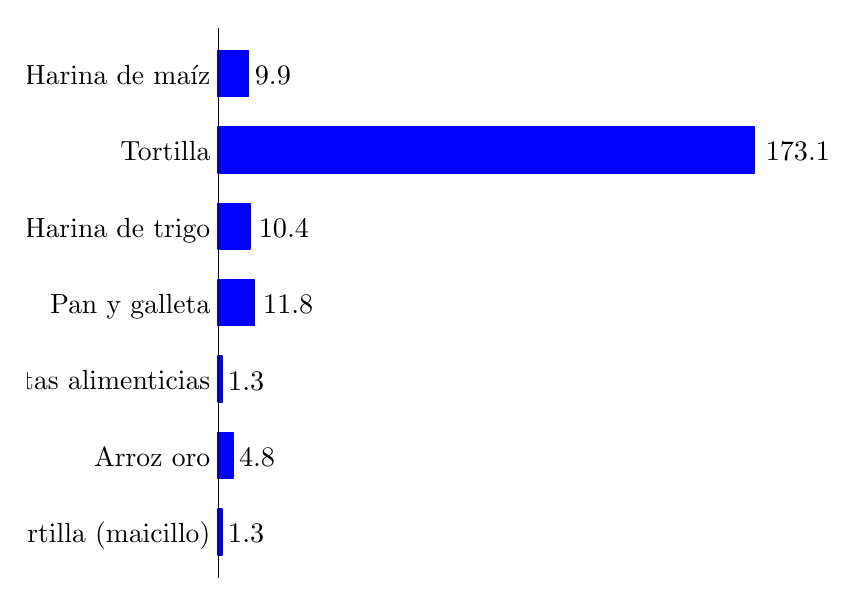
\begin{tikzpicture}[x=1pt,y=1pt]  % Created by tikzDevice version 0.9 on 2016-03-03 04:15:33
% !TEX encoding = UTF-8 Unicode
\definecolor{fillColor}{RGB}{255,255,255}
\path[use as bounding box,fill=fillColor,fill opacity=0.00] (0,0) rectangle (289.08,198.74);
\begin{scope}
\path[clip] (  0.00,  0.00) rectangle (289.08,198.74);

\path[] (  0.00,  0.00) rectangle (289.08,198.74);
\end{scope}
\begin{scope}
\path[clip] (  0.00,  0.00) rectangle (289.08,198.74);

\path[] ( 68.75,  0.00) rectangle (262.69,198.74);

\path[] ( 68.75, 16.56) --
	(262.69, 16.56);

\path[] ( 68.75, 44.16) --
	(262.69, 44.16);

\path[] ( 68.75, 71.77) --
	(262.69, 71.77);

\path[] ( 68.75, 99.37) --
	(262.69, 99.37);

\path[] ( 68.75,126.97) --
	(262.69,126.97);

\path[] ( 68.75,154.58) --
	(262.69,154.58);

\path[] ( 68.75,182.18) --
	(262.69,182.18);
\definecolor{drawColor}{RGB}{0,0,255}
\definecolor{fillColor}{RGB}{0,0,255}

\path[draw=drawColor,line width= 0.6pt,line join=round,fill=fillColor] ( 68.75,  8.28) rectangle ( 70.21, 24.84);

\path[draw=drawColor,line width= 0.6pt,line join=round,fill=fillColor] ( 68.75, 35.88) rectangle ( 74.13, 52.45);

\path[draw=drawColor,line width= 0.6pt,line join=round,fill=fillColor] ( 68.75, 63.49) rectangle ( 70.21, 80.05);

\path[draw=drawColor,line width= 0.6pt,line join=round,fill=fillColor] ( 68.75, 91.09) rectangle ( 81.98,107.65);

\path[draw=drawColor,line width= 0.6pt,line join=round,fill=fillColor] ( 68.75,118.69) rectangle ( 80.41,135.26);

\path[draw=drawColor,line width= 0.6pt,line join=round,fill=fillColor] ( 68.75,146.30) rectangle (262.69,162.86);

\path[draw=drawColor,line width= 0.6pt,line join=round,fill=fillColor] ( 68.75,173.90) rectangle ( 79.85,190.46);
\definecolor{drawColor}{RGB}{0,0,0}

\path[draw=drawColor,line width= 0.1pt,line join=round] ( 68.75,  0.00) -- ( 68.75,198.74);

\node[text=drawColor,anchor=base west,inner sep=0pt, outer sep=0pt, scale=  1.02] at ( 72.45, 12.59) {1.3};

\node[text=drawColor,anchor=base west,inner sep=0pt, outer sep=0pt, scale=  1.02] at ( 76.37, 40.19) {4.8};

\node[text=drawColor,anchor=base west,inner sep=0pt, outer sep=0pt, scale=  1.02] at ( 72.45, 67.80) {1.3};

\node[text=drawColor,anchor=base west,inner sep=0pt, outer sep=0pt, scale=  1.02] at ( 85.10, 95.40) {11.8};

\node[text=drawColor,anchor=base west,inner sep=0pt, outer sep=0pt, scale=  1.02] at ( 83.53,123.00) {10.4};

\node[text=drawColor,anchor=base west,inner sep=0pt, outer sep=0pt, scale=  1.02] at (266.71,150.61) {173.1};

\node[text=drawColor,anchor=base west,inner sep=0pt, outer sep=0pt, scale=  1.02] at ( 82.08,178.21) {9.9};

\path[] ( 68.75,  0.00) rectangle (262.69,198.74);
\end{scope}
\begin{scope}
\path[clip] (  0.00,  0.00) rectangle (289.08,198.74);

\path[] ( 68.75,  0.00) --
	( 68.75,198.74);
\end{scope}
\begin{scope}
\path[clip] (  0.00,  0.00) rectangle (289.08,198.74);
\definecolor{drawColor}{RGB}{0,0,0}

\node[text=drawColor,anchor=base east,inner sep=0pt, outer sep=0pt, scale=  1.00] at ( 66.00, 12.65) {Tortilla (maicillo)};

\node[text=drawColor,anchor=base east,inner sep=0pt, outer sep=0pt, scale=  1.00] at ( 66.00, 40.26) {Arroz oro};

\node[text=drawColor,anchor=base east,inner sep=0pt, outer sep=0pt, scale=  1.00] at ( 66.00, 67.86) {Pastas alimenticias};

\node[text=drawColor,anchor=base east,inner sep=0pt, outer sep=0pt, scale=  1.00] at ( 66.00, 95.46) {Pan y galleta};

\node[text=drawColor,anchor=base east,inner sep=0pt, outer sep=0pt, scale=  1.00] at ( 66.00,123.07) {Harina de trigo};

\node[text=drawColor,anchor=base east,inner sep=0pt, outer sep=0pt, scale=  1.00] at ( 66.00,150.67) {Tortilla};

\node[text=drawColor,anchor=base east,inner sep=0pt, outer sep=0pt, scale=  1.00] at ( 66.00,178.27) {Harina de maíz};
\end{scope}
\begin{scope}
\path[clip] (  0.00,  0.00) rectangle (289.08,198.74);

\path[] ( 66.00, 16.56) --
	( 68.75, 16.56);

\path[] ( 66.00, 44.16) --
	( 68.75, 44.16);

\path[] ( 66.00, 71.77) --
	( 68.75, 71.77);

\path[] ( 66.00, 99.37) --
	( 68.75, 99.37);

\path[] ( 66.00,126.97) --
	( 68.75,126.97);

\path[] ( 66.00,154.58) --
	( 68.75,154.58);

\path[] ( 66.00,182.18) --
	( 68.75,182.18);
\end{scope}
  \end{tikzpicture}}%
{%
	INE y MAGA} %

%#########################18########################

\cajita{%
	Disponibilidad per cápita de Leguminosas, azúcares yo tubérculos }%
{%
}%
{%
	Disponibilidad per cápita de Leguminosas, azúcares yo tubérculos  } %
{%
	República de Guatemala, 2013 , en kilogramos } %
{%
	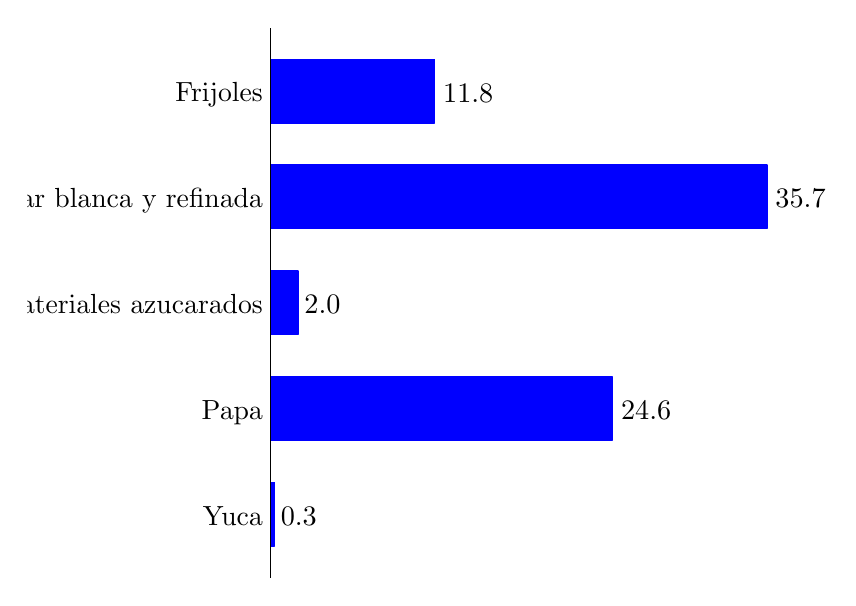
\begin{tikzpicture}[x=1pt,y=1pt]  % Created by tikzDevice version 0.9 on 2016-03-03 04:15:34
% !TEX encoding = UTF-8 Unicode
\definecolor{fillColor}{RGB}{255,255,255}
\path[use as bounding box,fill=fillColor,fill opacity=0.00] (0,0) rectangle (289.08,198.74);
\begin{scope}
\path[clip] (  0.00,  0.00) rectangle (289.08,198.74);

\path[] (  0.00,  0.00) rectangle (289.08,198.74);
\end{scope}
\begin{scope}
\path[clip] (  0.00,  0.00) rectangle (289.08,198.74);

\path[] ( 87.72,  0.00) rectangle (267.09,198.74);

\path[] ( 87.72, 22.93) --
	(267.09, 22.93);

\path[] ( 87.72, 61.15) --
	(267.09, 61.15);

\path[] ( 87.72, 99.37) --
	(267.09, 99.37);

\path[] ( 87.72,137.59) --
	(267.09,137.59);

\path[] ( 87.72,175.81) --
	(267.09,175.81);
\definecolor{drawColor}{RGB}{0,0,255}
\definecolor{fillColor}{RGB}{0,0,255}

\path[draw=drawColor,line width= 0.6pt,line join=round,fill=fillColor] ( 87.72, 11.47) rectangle ( 89.23, 34.40);

\path[draw=drawColor,line width= 0.6pt,line join=round,fill=fillColor] ( 87.72, 49.69) rectangle (211.32, 72.62);

\path[draw=drawColor,line width= 0.6pt,line join=round,fill=fillColor] ( 87.72, 87.91) rectangle ( 97.77,110.84);

\path[draw=drawColor,line width= 0.6pt,line join=round,fill=fillColor] ( 87.72,126.13) rectangle (267.09,149.06);

\path[draw=drawColor,line width= 0.6pt,line join=round,fill=fillColor] ( 87.72,164.34) rectangle (147.01,187.28);
\definecolor{drawColor}{RGB}{0,0,0}

\path[draw=drawColor,line width= 0.1pt,line join=round] ( 87.72,  0.00) -- ( 87.72,198.74);

\node[text=drawColor,anchor=base west,inner sep=0pt, outer sep=0pt, scale=  1.02] at ( 91.46, 18.96) {0.3};

\node[text=drawColor,anchor=base west,inner sep=0pt, outer sep=0pt, scale=  1.02] at (214.44, 57.18) {24.6};

\node[text=drawColor,anchor=base west,inner sep=0pt, outer sep=0pt, scale=  1.02] at (100.01, 95.40) {2.0};

\node[text=drawColor,anchor=base west,inner sep=0pt, outer sep=0pt, scale=  1.02] at (270.21,133.62) {35.7};

\node[text=drawColor,anchor=base west,inner sep=0pt, outer sep=0pt, scale=  1.02] at (150.13,171.84) {11.8};

\path[] ( 87.72,  0.00) rectangle (267.09,198.74);
\end{scope}
\begin{scope}
\path[clip] (  0.00,  0.00) rectangle (289.08,198.74);

\path[] ( 87.72,  0.00) --
	( 87.72,198.74);
\end{scope}
\begin{scope}
\path[clip] (  0.00,  0.00) rectangle (289.08,198.74);
\definecolor{drawColor}{RGB}{0,0,0}

\node[text=drawColor,anchor=base east,inner sep=0pt, outer sep=0pt, scale=  1.00] at ( 84.97, 19.02) {Yuca};

\node[text=drawColor,anchor=base east,inner sep=0pt, outer sep=0pt, scale=  1.00] at ( 84.97, 57.24) {Papa};

\node[text=drawColor,anchor=base east,inner sep=0pt, outer sep=0pt, scale=  1.00] at ( 84.97, 95.46) {Materiales azucarados};

\node[text=drawColor,anchor=base east,inner sep=0pt, outer sep=0pt, scale=  1.00] at ( 84.97,133.68) {Azúcar blanca y refinada};

\node[text=drawColor,anchor=base east,inner sep=0pt, outer sep=0pt, scale=  1.00] at ( 84.97,171.90) {Frijoles};
\end{scope}
\begin{scope}
\path[clip] (  0.00,  0.00) rectangle (289.08,198.74);

\path[] ( 84.97, 22.93) --
	( 87.72, 22.93);

\path[] ( 84.97, 61.15) --
	( 87.72, 61.15);

\path[] ( 84.97, 99.37) --
	( 87.72, 99.37);

\path[] ( 84.97,137.59) --
	( 87.72,137.59);

\path[] ( 84.97,175.81) --
	( 87.72,175.81);
\end{scope}
  \end{tikzpicture}}%
{%
	INE y MAGA} %

%#########################19########################

\cajita{%
	Disponibilidad per cápita de Hortalizas}%
{%
}%
{%
	Disponibilidad per cápita de Hortalizas } %
{%
	República de Guatemala, 2013 , en kilogramos } %
{%
	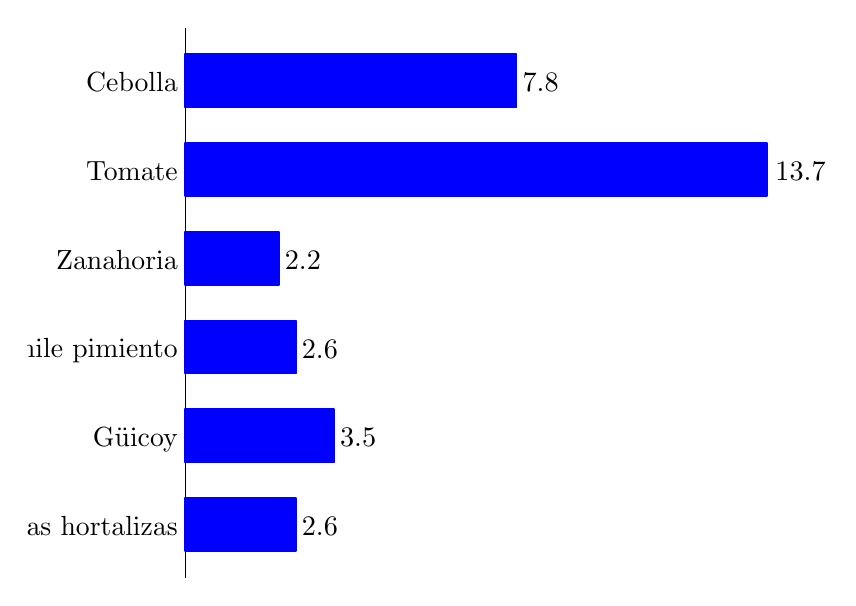
\begin{tikzpicture}[x=1pt,y=1pt]  % Created by tikzDevice version 0.9 on 2016-03-03 04:15:34
% !TEX encoding = UTF-8 Unicode
\definecolor{fillColor}{RGB}{255,255,255}
\path[use as bounding box,fill=fillColor,fill opacity=0.00] (0,0) rectangle (289.08,198.74);
\begin{scope}
\path[clip] (  0.00,  0.00) rectangle (289.08,198.74);

\path[] (  0.00,  0.00) rectangle (289.08,198.74);
\end{scope}
\begin{scope}
\path[clip] (  0.00,  0.00) rectangle (289.08,198.74);

\path[] ( 56.96,  0.00) rectangle (267.09,198.74);

\path[] ( 56.96, 19.23) --
	(267.09, 19.23);

\path[] ( 56.96, 51.29) --
	(267.09, 51.29);

\path[] ( 56.96, 83.34) --
	(267.09, 83.34);

\path[] ( 56.96,115.40) --
	(267.09,115.40);

\path[] ( 56.96,147.45) --
	(267.09,147.45);

\path[] ( 56.96,179.51) --
	(267.09,179.51);
\definecolor{drawColor}{RGB}{0,0,255}
\definecolor{fillColor}{RGB}{0,0,255}

\path[draw=drawColor,line width= 0.6pt,line join=round,fill=fillColor] ( 56.96,  9.62) rectangle ( 96.84, 28.85);

\path[draw=drawColor,line width= 0.6pt,line join=round,fill=fillColor] ( 56.96, 41.67) rectangle (110.64, 60.90);

\path[draw=drawColor,line width= 0.6pt,line join=round,fill=fillColor] ( 56.96, 73.73) rectangle ( 96.84, 92.96);

\path[draw=drawColor,line width= 0.6pt,line join=round,fill=fillColor] ( 56.96,105.78) rectangle ( 90.70,125.02);

\path[draw=drawColor,line width= 0.6pt,line join=round,fill=fillColor] ( 56.96,137.84) rectangle (267.09,157.07);

\path[draw=drawColor,line width= 0.6pt,line join=round,fill=fillColor] ( 56.96,169.89) rectangle (176.59,189.13);
\definecolor{drawColor}{RGB}{0,0,0}

\path[draw=drawColor,line width= 0.1pt,line join=round] ( 56.96,  0.00) -- ( 56.96,198.74);

\node[text=drawColor,anchor=base west,inner sep=0pt, outer sep=0pt, scale=  1.02] at ( 99.08, 15.26) {2.6};

\node[text=drawColor,anchor=base west,inner sep=0pt, outer sep=0pt, scale=  1.02] at (112.88, 47.32) {3.5};

\node[text=drawColor,anchor=base west,inner sep=0pt, outer sep=0pt, scale=  1.02] at ( 99.08, 79.37) {2.6};

\node[text=drawColor,anchor=base west,inner sep=0pt, outer sep=0pt, scale=  1.02] at ( 92.94,111.43) {2.2};

\node[text=drawColor,anchor=base west,inner sep=0pt, outer sep=0pt, scale=  1.02] at (270.21,143.48) {13.7};

\node[text=drawColor,anchor=base west,inner sep=0pt, outer sep=0pt, scale=  1.02] at (178.83,175.54) {7.8};

\path[] ( 56.96,  0.00) rectangle (267.09,198.74);
\end{scope}
\begin{scope}
\path[clip] (  0.00,  0.00) rectangle (289.08,198.74);

\path[] ( 56.96,  0.00) --
	( 56.96,198.74);
\end{scope}
\begin{scope}
\path[clip] (  0.00,  0.00) rectangle (289.08,198.74);
\definecolor{drawColor}{RGB}{0,0,0}

\node[text=drawColor,anchor=base east,inner sep=0pt, outer sep=0pt, scale=  1.00] at ( 54.21, 15.32) {Otras hortalizas};

\node[text=drawColor,anchor=base east,inner sep=0pt, outer sep=0pt, scale=  1.00] at ( 54.21, 47.38) {Güicoy};

\node[text=drawColor,anchor=base east,inner sep=0pt, outer sep=0pt, scale=  1.00] at ( 54.21, 79.44) {Chile pimiento};

\node[text=drawColor,anchor=base east,inner sep=0pt, outer sep=0pt, scale=  1.00] at ( 54.21,111.49) {Zanahoria};

\node[text=drawColor,anchor=base east,inner sep=0pt, outer sep=0pt, scale=  1.00] at ( 54.21,143.55) {Tomate};

\node[text=drawColor,anchor=base east,inner sep=0pt, outer sep=0pt, scale=  1.00] at ( 54.21,175.60) {Cebolla};
\end{scope}
\begin{scope}
\path[clip] (  0.00,  0.00) rectangle (289.08,198.74);

\path[] ( 54.21, 19.23) --
	( 56.96, 19.23);

\path[] ( 54.21, 51.29) --
	( 56.96, 51.29);

\path[] ( 54.21, 83.34) --
	( 56.96, 83.34);

\path[] ( 54.21,115.40) --
	( 56.96,115.40);

\path[] ( 54.21,147.45) --
	( 56.96,147.45);

\path[] ( 54.21,179.51) --
	( 56.96,179.51);
\end{scope}
  \end{tikzpicture}}%
{%
	INE y MAGA} %

%#########################20########################

\cajita{%
	Disponibilidad per cápita de Frutas}%
{%
}%
{%
	Disponibilidad per cápita de Frutas } %
{%
	República de Guatemala, 2013 , en kilogramos } %
{%
	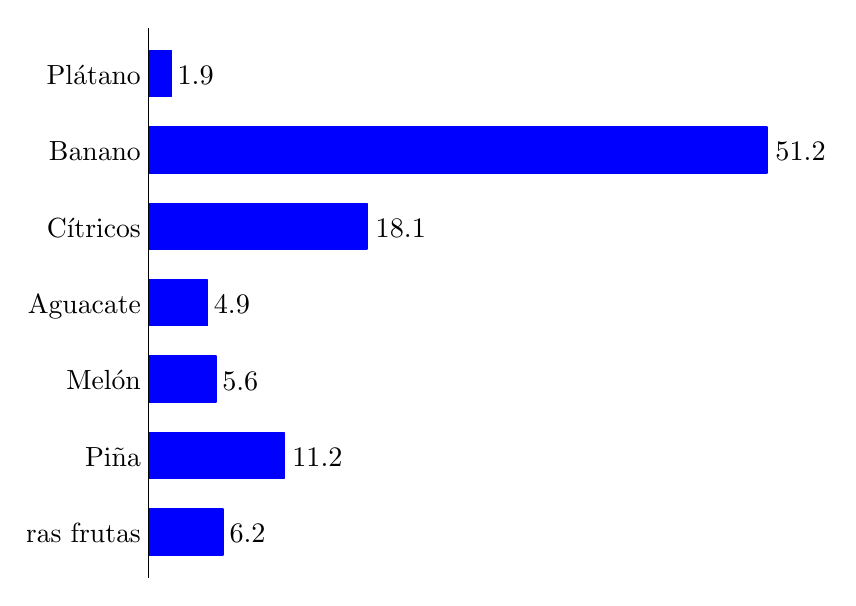
\begin{tikzpicture}[x=1pt,y=1pt]  % Created by tikzDevice version 0.9 on 2016-03-03 04:15:36
% !TEX encoding = UTF-8 Unicode
\definecolor{fillColor}{RGB}{255,255,255}
\path[use as bounding box,fill=fillColor,fill opacity=0.00] (0,0) rectangle (289.08,198.74);
\begin{scope}
\path[clip] (  0.00,  0.00) rectangle (289.08,198.74);

\path[] (  0.00,  0.00) rectangle (289.08,198.74);
\end{scope}
\begin{scope}
\path[clip] (  0.00,  0.00) rectangle (289.08,198.74);

\path[] ( 43.64,  0.00) rectangle (267.09,198.74);

\path[] ( 43.64, 16.56) --
	(267.09, 16.56);

\path[] ( 43.64, 44.16) --
	(267.09, 44.16);

\path[] ( 43.64, 71.77) --
	(267.09, 71.77);

\path[] ( 43.64, 99.37) --
	(267.09, 99.37);

\path[] ( 43.64,126.97) --
	(267.09,126.97);

\path[] ( 43.64,154.58) --
	(267.09,154.58);

\path[] ( 43.64,182.18) --
	(267.09,182.18);
\definecolor{drawColor}{RGB}{0,0,255}
\definecolor{fillColor}{RGB}{0,0,255}

\path[draw=drawColor,line width= 0.6pt,line join=round,fill=fillColor] ( 43.64,  8.28) rectangle ( 70.69, 24.84);

\path[draw=drawColor,line width= 0.6pt,line join=round,fill=fillColor] ( 43.64, 35.88) rectangle ( 92.52, 52.45);

\path[draw=drawColor,line width= 0.6pt,line join=round,fill=fillColor] ( 43.64, 63.49) rectangle ( 68.08, 80.05);

\path[draw=drawColor,line width= 0.6pt,line join=round,fill=fillColor] ( 43.64, 91.09) rectangle ( 65.02,107.65);

\path[draw=drawColor,line width= 0.6pt,line join=round,fill=fillColor] ( 43.64,118.69) rectangle (122.63,135.26);

\path[draw=drawColor,line width= 0.6pt,line join=round,fill=fillColor] ( 43.64,146.30) rectangle (267.09,162.86);

\path[draw=drawColor,line width= 0.6pt,line join=round,fill=fillColor] ( 43.64,173.90) rectangle ( 51.93,190.46);
\definecolor{drawColor}{RGB}{0,0,0}

\path[draw=drawColor,line width= 0.1pt,line join=round] ( 43.64,  0.00) -- ( 43.64,198.74);

\node[text=drawColor,anchor=base west,inner sep=0pt, outer sep=0pt, scale=  1.02] at ( 72.93, 12.59) {6.2};

\node[text=drawColor,anchor=base west,inner sep=0pt, outer sep=0pt, scale=  1.02] at ( 95.64, 40.19) {11.2};

\node[text=drawColor,anchor=base west,inner sep=0pt, outer sep=0pt, scale=  1.02] at ( 70.31, 67.80) {5.6};

\node[text=drawColor,anchor=base west,inner sep=0pt, outer sep=0pt, scale=  1.02] at ( 67.26, 95.40) {4.9};

\node[text=drawColor,anchor=base west,inner sep=0pt, outer sep=0pt, scale=  1.02] at (125.76,123.00) {18.1};

\node[text=drawColor,anchor=base west,inner sep=0pt, outer sep=0pt, scale=  1.02] at (270.21,150.61) {51.2};

\node[text=drawColor,anchor=base west,inner sep=0pt, outer sep=0pt, scale=  1.02] at ( 54.17,178.21) {1.9};

\path[] ( 43.64,  0.00) rectangle (267.09,198.74);
\end{scope}
\begin{scope}
\path[clip] (  0.00,  0.00) rectangle (289.08,198.74);

\path[] ( 43.64,  0.00) --
	( 43.64,198.74);
\end{scope}
\begin{scope}
\path[clip] (  0.00,  0.00) rectangle (289.08,198.74);
\definecolor{drawColor}{RGB}{0,0,0}

\node[text=drawColor,anchor=base east,inner sep=0pt, outer sep=0pt, scale=  1.00] at ( 40.89, 12.65) {Otras frutas};

\node[text=drawColor,anchor=base east,inner sep=0pt, outer sep=0pt, scale=  1.00] at ( 40.89, 40.26) {Piña};

\node[text=drawColor,anchor=base east,inner sep=0pt, outer sep=0pt, scale=  1.00] at ( 40.89, 67.86) {Melón};

\node[text=drawColor,anchor=base east,inner sep=0pt, outer sep=0pt, scale=  1.00] at ( 40.89, 95.46) {Aguacate};

\node[text=drawColor,anchor=base east,inner sep=0pt, outer sep=0pt, scale=  1.00] at ( 40.89,123.07) {Cítricos};

\node[text=drawColor,anchor=base east,inner sep=0pt, outer sep=0pt, scale=  1.00] at ( 40.89,150.67) {Banano};

\node[text=drawColor,anchor=base east,inner sep=0pt, outer sep=0pt, scale=  1.00] at ( 40.89,178.27) {Plátano};
\end{scope}
\begin{scope}
\path[clip] (  0.00,  0.00) rectangle (289.08,198.74);

\path[] ( 40.89, 16.56) --
	( 43.64, 16.56);

\path[] ( 40.89, 44.16) --
	( 43.64, 44.16);

\path[] ( 40.89, 71.77) --
	( 43.64, 71.77);

\path[] ( 40.89, 99.37) --
	( 43.64, 99.37);

\path[] ( 40.89,126.97) --
	( 43.64,126.97);

\path[] ( 40.89,154.58) --
	( 43.64,154.58);

\path[] ( 40.89,182.18) --
	( 43.64,182.18);
\end{scope}
  \end{tikzpicture}}%
{%
	INE y MAGA} %

%#########################21########################

\cajita{%
	Disponibilidad per cápita de carnes}%
{%
}%
{%
	Disponibilidad per cápita de carnes } %
{%
	República de Guatemala, 2013 , en kilogramos } %
{%
	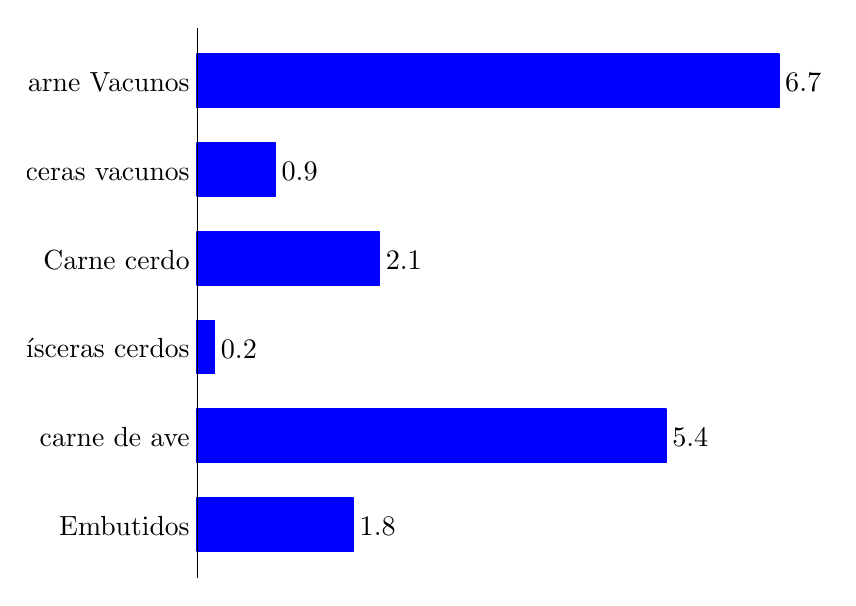
\begin{tikzpicture}[x=1pt,y=1pt]  % Created by tikzDevice version 0.9 on 2016-03-03 04:15:57
% !TEX encoding = UTF-8 Unicode
\definecolor{fillColor}{RGB}{255,255,255}
\path[use as bounding box,fill=fillColor,fill opacity=0.00] (0,0) rectangle (289.08,198.74);
\begin{scope}
\path[clip] (  0.00,  0.00) rectangle (289.08,198.74);

\path[] (  0.00,  0.00) rectangle (289.08,198.74);
\end{scope}
\begin{scope}
\path[clip] (  0.00,  0.00) rectangle (289.08,198.74);

\path[] ( 61.28,  0.00) rectangle (271.48,198.74);

\path[] ( 61.28, 19.23) --
	(271.48, 19.23);

\path[] ( 61.28, 51.29) --
	(271.48, 51.29);

\path[] ( 61.28, 83.34) --
	(271.48, 83.34);

\path[] ( 61.28,115.40) --
	(271.48,115.40);

\path[] ( 61.28,147.45) --
	(271.48,147.45);

\path[] ( 61.28,179.51) --
	(271.48,179.51);
\definecolor{drawColor}{RGB}{0,0,255}
\definecolor{fillColor}{RGB}{0,0,255}

\path[draw=drawColor,line width= 0.6pt,line join=round,fill=fillColor] ( 61.28,  9.62) rectangle (117.75, 28.85);

\path[draw=drawColor,line width= 0.6pt,line join=round,fill=fillColor] ( 61.28, 41.67) rectangle (230.70, 60.90);

\path[draw=drawColor,line width= 0.6pt,line join=round,fill=fillColor] ( 61.28, 73.73) rectangle ( 67.55, 92.96);

\path[draw=drawColor,line width= 0.6pt,line join=round,fill=fillColor] ( 61.28,105.78) rectangle (127.16,125.02);

\path[draw=drawColor,line width= 0.6pt,line join=round,fill=fillColor] ( 61.28,137.84) rectangle ( 89.52,157.07);

\path[draw=drawColor,line width= 0.6pt,line join=round,fill=fillColor] ( 61.28,169.89) rectangle (271.48,189.13);
\definecolor{drawColor}{RGB}{0,0,0}

\path[draw=drawColor,line width= 0.1pt,line join=round] ( 61.28,  0.00) -- ( 61.28,198.74);

\node[text=drawColor,anchor=base west,inner sep=0pt, outer sep=0pt, scale=  1.02] at (119.99, 15.26) {1.8};

\node[text=drawColor,anchor=base west,inner sep=0pt, outer sep=0pt, scale=  1.02] at (232.93, 47.32) {5.4};

\node[text=drawColor,anchor=base west,inner sep=0pt, outer sep=0pt, scale=  1.02] at ( 69.79, 79.37) {0.2};

\node[text=drawColor,anchor=base west,inner sep=0pt, outer sep=0pt, scale=  1.02] at (129.40,111.43) {2.1};

\node[text=drawColor,anchor=base west,inner sep=0pt, outer sep=0pt, scale=  1.02] at ( 91.75,143.48) {0.9};

\node[text=drawColor,anchor=base west,inner sep=0pt, outer sep=0pt, scale=  1.02] at (273.72,175.54) {6.7};

\path[] ( 61.28,  0.00) rectangle (271.48,198.74);
\end{scope}
\begin{scope}
\path[clip] (  0.00,  0.00) rectangle (289.08,198.74);

\path[] ( 61.28,  0.00) --
	( 61.28,198.74);
\end{scope}
\begin{scope}
\path[clip] (  0.00,  0.00) rectangle (289.08,198.74);
\definecolor{drawColor}{RGB}{0,0,0}

\node[text=drawColor,anchor=base east,inner sep=0pt, outer sep=0pt, scale=  1.00] at ( 58.53, 15.32) {Embutidos };

\node[text=drawColor,anchor=base east,inner sep=0pt, outer sep=0pt, scale=  1.00] at ( 58.53, 47.38) {carne de ave};

\node[text=drawColor,anchor=base east,inner sep=0pt, outer sep=0pt, scale=  1.00] at ( 58.53, 79.44) {Vísceras cerdos};

\node[text=drawColor,anchor=base east,inner sep=0pt, outer sep=0pt, scale=  1.00] at ( 58.53,111.49) {Carne cerdo};

\node[text=drawColor,anchor=base east,inner sep=0pt, outer sep=0pt, scale=  1.00] at ( 58.53,143.55) {Visceras vacunos};

\node[text=drawColor,anchor=base east,inner sep=0pt, outer sep=0pt, scale=  1.00] at ( 58.53,175.60) {Carne Vacunos};
\end{scope}
\begin{scope}
\path[clip] (  0.00,  0.00) rectangle (289.08,198.74);

\path[] ( 58.53, 19.23) --
	( 61.28, 19.23);

\path[] ( 58.53, 51.29) --
	( 61.28, 51.29);

\path[] ( 58.53, 83.34) --
	( 61.28, 83.34);

\path[] ( 58.53,115.40) --
	( 61.28,115.40);

\path[] ( 58.53,147.45) --
	( 61.28,147.45);

\path[] ( 58.53,179.51) --
	( 61.28,179.51);
\end{scope}
  \end{tikzpicture}}%
{%
	INE y MAGA} %

%#########################22########################

\cajita{%
	Disponibilidad per cápita de huevo, pescado y mariscos}%
{%
}%
{%
	Disponibilidad per cápita de huevo, pescado y mariscos } %
{%
	República de Guatemala, 2013 , en kilogramos } %
{%
	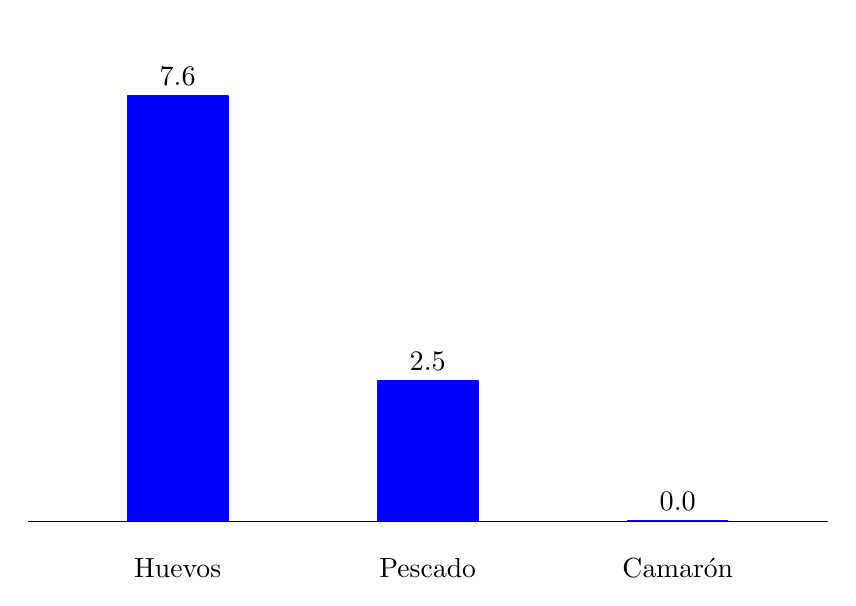
\begin{tikzpicture}[x=1pt,y=1pt]  % Created by tikzDevice version 0.9 on 2016-03-03 04:16:14
% !TEX encoding = UTF-8 Unicode
\definecolor{fillColor}{RGB}{255,255,255}
\path[use as bounding box,fill=fillColor,fill opacity=0.00] (0,0) rectangle (289.08,198.74);
\begin{scope}
\path[clip] (  0.00,  0.00) rectangle (289.08,198.74);

\path[] (  0.00,  0.00) rectangle (289.08,198.74);
\end{scope}
\begin{scope}
\path[clip] (  0.00,  0.00) rectangle (289.08,198.74);

\path[] (  0.00, 12.77) rectangle (289.08,181.67);

\path[] ( 54.20, 12.77) --
	( 54.20,181.67);

\path[] (144.54, 12.77) --
	(144.54,181.67);

\path[] (234.88, 12.77) --
	(234.88,181.67);
\definecolor{drawColor}{RGB}{0,0,255}
\definecolor{fillColor}{RGB}{0,0,255}

\path[draw=drawColor,line width= 0.6pt,line join=round,fill=fillColor] ( 36.13, 20.44) rectangle ( 72.27,173.99);

\path[draw=drawColor,line width= 0.6pt,line join=round,fill=fillColor] (126.47, 20.44) rectangle (162.61, 70.95);

\path[draw=drawColor,line width= 0.6pt,line join=round,fill=fillColor] (216.81, 20.44) rectangle (252.95, 20.44);
\definecolor{drawColor}{RGB}{0,0,0}

\path[draw=drawColor,line width= 0.1pt,line join=round] (  0.00, 20.44) -- (289.08, 20.44);

\node[text=drawColor,anchor=base,inner sep=0pt, outer sep=0pt, scale=  1.02] at ( 54.20,177.96) {7.6};

\node[text=drawColor,anchor=base,inner sep=0pt, outer sep=0pt, scale=  1.02] at (144.54, 74.92) {2.5};

\node[text=drawColor,anchor=base,inner sep=0pt, outer sep=0pt, scale=  1.02] at (234.88, 24.42) {0.0};

\path[] (  0.00, 12.77) rectangle (289.08,181.67);
\end{scope}
\begin{scope}
\path[clip] (  0.00,  0.00) rectangle (289.08,198.74);

\path[] (  0.00, 12.77) --
	(289.08, 12.77);
\end{scope}
\begin{scope}
\path[clip] (  0.00,  0.00) rectangle (289.08,198.74);

\path[] ( 54.20, 10.02) --
	( 54.20, 12.77);

\path[] (144.54, 10.02) --
	(144.54, 12.77);

\path[] (234.88, 10.02) --
	(234.88, 12.77);
\end{scope}
\begin{scope}
\path[clip] (  0.00,  0.00) rectangle (289.08,198.74);
\definecolor{drawColor}{RGB}{0,0,0}

\node[text=drawColor,anchor=base,inner sep=0pt, outer sep=0pt, scale=  1.00] at ( 54.20, -0.00) {Huevos};

\node[text=drawColor,anchor=base,inner sep=0pt, outer sep=0pt, scale=  1.00] at (144.54, -0.00) {Pescado};

\node[text=drawColor,anchor=base,inner sep=0pt, outer sep=0pt, scale=  1.00] at (234.88, -0.00) {Camarón};
\end{scope}
  \end{tikzpicture}}%
{%
	INE y MAGA} %

%#########################23########################

\cajita{%
	Disponibilidad per cápita de productos lácteos}%
{%
}%
{%
	Disponibilidad per cápita de productos lácteos} %
{%
	República de Guatemala, 2013 , en kilogramos } %
{%
	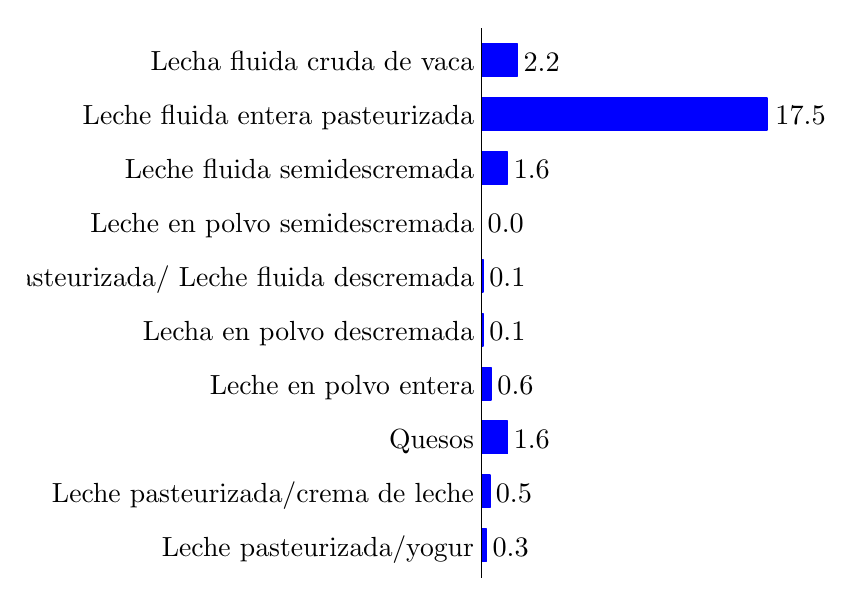
\begin{tikzpicture}[x=1pt,y=1pt]  % Created by tikzDevice version 0.9 on 2016-03-03 04:16:23
% !TEX encoding = UTF-8 Unicode
\definecolor{fillColor}{RGB}{255,255,255}
\path[use as bounding box,fill=fillColor,fill opacity=0.00] (0,0) rectangle (289.08,198.74);
\begin{scope}
\path[clip] (  0.00,  0.00) rectangle (289.08,198.74);

\path[] (  0.00,  0.00) rectangle (289.08,198.74);
\end{scope}
\begin{scope}
\path[clip] (  0.00,  0.00) rectangle (289.08,198.74);

\path[] (164.00,  0.00) rectangle (267.09,198.74);

\path[] (164.00, 11.69) --
	(267.09, 11.69);

\path[] (164.00, 31.18) --
	(267.09, 31.18);

\path[] (164.00, 50.66) --
	(267.09, 50.66);

\path[] (164.00, 70.14) --
	(267.09, 70.14);

\path[] (164.00, 89.63) --
	(267.09, 89.63);

\path[] (164.00,109.11) --
	(267.09,109.11);

\path[] (164.00,128.60) --
	(267.09,128.60);

\path[] (164.00,148.08) --
	(267.09,148.08);

\path[] (164.00,167.57) --
	(267.09,167.57);

\path[] (164.00,187.05) --
	(267.09,187.05);
\definecolor{drawColor}{RGB}{0,0,255}
\definecolor{fillColor}{RGB}{0,0,255}

\path[draw=drawColor,line width= 0.6pt,line join=round,fill=fillColor] (164.00,  5.85) rectangle (165.77, 17.54);

\path[draw=drawColor,line width= 0.6pt,line join=round,fill=fillColor] (164.00, 25.33) rectangle (166.95, 37.02);

\path[draw=drawColor,line width= 0.6pt,line join=round,fill=fillColor] (164.00, 44.81) rectangle (173.43, 56.51);

\path[draw=drawColor,line width= 0.6pt,line join=round,fill=fillColor] (164.00, 64.30) rectangle (167.53, 75.99);

\path[draw=drawColor,line width= 0.6pt,line join=round,fill=fillColor] (164.00, 83.78) rectangle (164.59, 95.47);

\path[draw=drawColor,line width= 0.6pt,line join=round,fill=fillColor] (164.00,103.27) rectangle (164.59,114.96);

\path[draw=drawColor,line width= 0.6pt,line join=round,fill=fillColor] (164.00,122.75) rectangle (164.00,134.44);

\path[draw=drawColor,line width= 0.6pt,line join=round,fill=fillColor] (164.00,142.24) rectangle (173.43,153.93);

\path[draw=drawColor,line width= 0.6pt,line join=round,fill=fillColor] (164.00,161.72) rectangle (267.09,173.41);

\path[draw=drawColor,line width= 0.6pt,line join=round,fill=fillColor] (164.00,181.21) rectangle (176.96,192.90);
\definecolor{drawColor}{RGB}{0,0,0}

\path[draw=drawColor,line width= 0.1pt,line join=round] (164.00,  0.00) -- (164.00,198.74);

\node[text=drawColor,anchor=base west,inner sep=0pt, outer sep=0pt, scale=  1.02] at (168.01,  7.72) {0.3};

\node[text=drawColor,anchor=base west,inner sep=0pt, outer sep=0pt, scale=  1.02] at (169.18, 27.20) {0.5};

\node[text=drawColor,anchor=base west,inner sep=0pt, outer sep=0pt, scale=  1.02] at (175.66, 46.69) {1.6};

\node[text=drawColor,anchor=base west,inner sep=0pt, outer sep=0pt, scale=  1.02] at (169.77, 66.17) {0.6};

\node[text=drawColor,anchor=base west,inner sep=0pt, outer sep=0pt, scale=  1.02] at (166.83, 85.66) {0.1};

\node[text=drawColor,anchor=base west,inner sep=0pt, outer sep=0pt, scale=  1.02] at (166.83,105.14) {0.1};

\node[text=drawColor,anchor=base west,inner sep=0pt, outer sep=0pt, scale=  1.02] at (166.24,124.63) {0.0};

\node[text=drawColor,anchor=base west,inner sep=0pt, outer sep=0pt, scale=  1.02] at (175.66,144.11) {1.6};

\node[text=drawColor,anchor=base west,inner sep=0pt, outer sep=0pt, scale=  1.02] at (270.21,163.60) {17.5};

\node[text=drawColor,anchor=base west,inner sep=0pt, outer sep=0pt, scale=  1.02] at (179.20,183.08) {2.2};

\path[] (164.00,  0.00) rectangle (267.09,198.74);
\end{scope}
\begin{scope}
\path[clip] (  0.00,  0.00) rectangle (289.08,198.74);

\path[] (164.00,  0.00) --
	(164.00,198.74);
\end{scope}
\begin{scope}
\path[clip] (  0.00,  0.00) rectangle (289.08,198.74);
\definecolor{drawColor}{RGB}{0,0,0}

\node[text=drawColor,anchor=base east,inner sep=0pt, outer sep=0pt, scale=  1.00] at (161.25,  7.78) {Leche pasteurizada/yogur};

\node[text=drawColor,anchor=base east,inner sep=0pt, outer sep=0pt, scale=  1.00] at (161.25, 27.27) {Leche pasteurizada/crema de leche};

\node[text=drawColor,anchor=base east,inner sep=0pt, outer sep=0pt, scale=  1.00] at (161.25, 46.75) {Quesos};

\node[text=drawColor,anchor=base east,inner sep=0pt, outer sep=0pt, scale=  1.00] at (161.25, 66.24) {Leche en polvo entera };

\node[text=drawColor,anchor=base east,inner sep=0pt, outer sep=0pt, scale=  1.00] at (161.25, 85.72) {Lecha en polvo descremada};

\node[text=drawColor,anchor=base east,inner sep=0pt, outer sep=0pt, scale=  1.00] at (161.25,105.21) {Leche pasteurizada/ Leche fluida descremada};

\node[text=drawColor,anchor=base east,inner sep=0pt, outer sep=0pt, scale=  1.00] at (161.25,124.69) {Leche en polvo semidescremada};

\node[text=drawColor,anchor=base east,inner sep=0pt, outer sep=0pt, scale=  1.00] at (161.25,144.17) {Leche fluida semidescremada};

\node[text=drawColor,anchor=base east,inner sep=0pt, outer sep=0pt, scale=  1.00] at (161.25,163.66) {Leche fluida entera pasteurizada};

\node[text=drawColor,anchor=base east,inner sep=0pt, outer sep=0pt, scale=  1.00] at (161.25,183.14) {Lecha fluida cruda de vaca};
\end{scope}
\begin{scope}
\path[clip] (  0.00,  0.00) rectangle (289.08,198.74);

\path[] (161.25, 11.69) --
	(164.00, 11.69);

\path[] (161.25, 31.18) --
	(164.00, 31.18);

\path[] (161.25, 50.66) --
	(164.00, 50.66);

\path[] (161.25, 70.14) --
	(164.00, 70.14);

\path[] (161.25, 89.63) --
	(164.00, 89.63);

\path[] (161.25,109.11) --
	(164.00,109.11);

\path[] (161.25,128.60) --
	(164.00,128.60);

\path[] (161.25,148.08) --
	(164.00,148.08);

\path[] (161.25,167.57) --
	(164.00,167.57);

\path[] (161.25,187.05) --
	(164.00,187.05);
\end{scope}
  \end{tikzpicture}}%
{%
	INE y MAGA} %


%#########################24########################

\cajita{%
	Disponibilidad per cápita de aceites y grasas}%
{%
}%
{%
	Disponibilidad per cápita de aceites y grasas} %
{%
	República de Guatemala, 2013 , en kilogramos } %
{%
	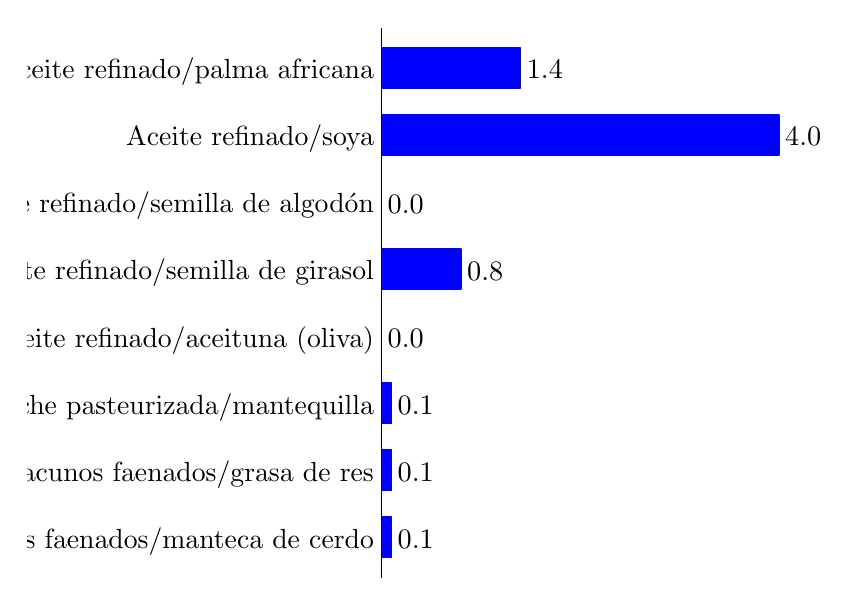
\begin{tikzpicture}[x=1pt,y=1pt]  % Created by tikzDevice version 0.9 on 2016-03-03 04:16:46
% !TEX encoding = UTF-8 Unicode
\definecolor{fillColor}{RGB}{255,255,255}
\path[use as bounding box,fill=fillColor,fill opacity=0.00] (0,0) rectangle (289.08,198.74);
\begin{scope}
\path[clip] (  0.00,  0.00) rectangle (289.08,198.74);

\path[] ( -0.00,  0.00) rectangle (289.08,198.74);
\end{scope}
\begin{scope}
\path[clip] (  0.00,  0.00) rectangle (289.08,198.74);

\path[] (127.86,  0.00) rectangle (271.48,198.74);

\path[] (127.86, 14.54) --
	(271.48, 14.54);

\path[] (127.86, 38.78) --
	(271.48, 38.78);

\path[] (127.86, 63.02) --
	(271.48, 63.02);

\path[] (127.86, 87.25) --
	(271.48, 87.25);

\path[] (127.86,111.49) --
	(271.48,111.49);

\path[] (127.86,135.73) --
	(271.48,135.73);

\path[] (127.86,159.96) --
	(271.48,159.96);

\path[] (127.86,184.20) --
	(271.48,184.20);
\definecolor{drawColor}{RGB}{0,0,255}
\definecolor{fillColor}{RGB}{0,0,255}

\path[draw=drawColor,line width= 0.6pt,line join=round,fill=fillColor] (127.86,  7.27) rectangle (131.45, 21.81);

\path[draw=drawColor,line width= 0.6pt,line join=round,fill=fillColor] (127.86, 31.51) rectangle (131.45, 46.05);

\path[draw=drawColor,line width= 0.6pt,line join=round,fill=fillColor] (127.86, 55.74) rectangle (131.45, 70.29);

\path[draw=drawColor,line width= 0.6pt,line join=round,fill=fillColor] (127.86, 79.98) rectangle (127.86, 94.52);

\path[draw=drawColor,line width= 0.6pt,line join=round,fill=fillColor] (127.86,104.22) rectangle (156.58,118.76);

\path[draw=drawColor,line width= 0.6pt,line join=round,fill=fillColor] (127.86,128.46) rectangle (127.86,143.00);

\path[draw=drawColor,line width= 0.6pt,line join=round,fill=fillColor] (127.86,152.69) rectangle (271.48,167.23);

\path[draw=drawColor,line width= 0.6pt,line join=round,fill=fillColor] (127.86,176.93) rectangle (178.13,191.47);
\definecolor{drawColor}{RGB}{0,0,0}

\path[draw=drawColor,line width= 0.1pt,line join=round] (127.86,  0.00) -- (127.86,198.74);

\node[text=drawColor,anchor=base west,inner sep=0pt, outer sep=0pt, scale=  1.02] at (133.69, 10.57) {0.1};

\node[text=drawColor,anchor=base west,inner sep=0pt, outer sep=0pt, scale=  1.02] at (133.69, 34.81) {0.1};

\node[text=drawColor,anchor=base west,inner sep=0pt, outer sep=0pt, scale=  1.02] at (133.69, 59.04) {0.1};

\node[text=drawColor,anchor=base west,inner sep=0pt, outer sep=0pt, scale=  1.02] at (130.10, 83.28) {0.0};

\node[text=drawColor,anchor=base west,inner sep=0pt, outer sep=0pt, scale=  1.02] at (158.82,107.52) {0.8};

\node[text=drawColor,anchor=base west,inner sep=0pt, outer sep=0pt, scale=  1.02] at (130.10,131.76) {0.0};

\node[text=drawColor,anchor=base west,inner sep=0pt, outer sep=0pt, scale=  1.02] at (273.72,155.99) {4.0};

\node[text=drawColor,anchor=base west,inner sep=0pt, outer sep=0pt, scale=  1.02] at (180.36,180.23) {1.4};

\path[] (127.86,  0.00) rectangle (271.48,198.74);
\end{scope}
\begin{scope}
\path[clip] (  0.00,  0.00) rectangle (289.08,198.74);

\path[] (127.86,  0.00) --
	(127.86,198.74);
\end{scope}
\begin{scope}
\path[clip] (  0.00,  0.00) rectangle (289.08,198.74);
\definecolor{drawColor}{RGB}{0,0,0}

\node[text=drawColor,anchor=base east,inner sep=0pt, outer sep=0pt, scale=  1.00] at (125.11, 10.63) {cerdos faenados/manteca de cerdo};

\node[text=drawColor,anchor=base east,inner sep=0pt, outer sep=0pt, scale=  1.00] at (125.11, 34.87) {Vacunos faenados/grasa de res};

\node[text=drawColor,anchor=base east,inner sep=0pt, outer sep=0pt, scale=  1.00] at (125.11, 59.11) {Leche pasteurizada/mantequilla};

\node[text=drawColor,anchor=base east,inner sep=0pt, outer sep=0pt, scale=  1.00] at (125.11, 83.34) {Aceite refinado/aceituna (oliva)};

\node[text=drawColor,anchor=base east,inner sep=0pt, outer sep=0pt, scale=  1.00] at (125.11,107.58) {Aceite refinado/semilla de girasol};

\node[text=drawColor,anchor=base east,inner sep=0pt, outer sep=0pt, scale=  1.00] at (125.11,131.82) {Aceite refinado/semilla de algodón};

\node[text=drawColor,anchor=base east,inner sep=0pt, outer sep=0pt, scale=  1.00] at (125.11,156.06) {Aceite refinado/soya};

\node[text=drawColor,anchor=base east,inner sep=0pt, outer sep=0pt, scale=  1.00] at (125.11,180.29) {Aceite refinado/palma africana};
\end{scope}
\begin{scope}
\path[clip] (  0.00,  0.00) rectangle (289.08,198.74);

\path[] (125.11, 14.54) --
	(127.86, 14.54);

\path[] (125.11, 38.78) --
	(127.86, 38.78);

\path[] (125.11, 63.02) --
	(127.86, 63.02);

\path[] (125.11, 87.25) --
	(127.86, 87.25);

\path[] (125.11,111.49) --
	(127.86,111.49);

\path[] (125.11,135.73) --
	(127.86,135.73);

\path[] (125.11,159.96) --
	(127.86,159.96);

\path[] (125.11,184.20) --
	(127.86,184.20);
\end{scope}
  \end{tikzpicture}}%
{%
	INE y MAGA} %

%#########################25########################

\cajita{%
	Disponibilidad per cápita de alimentos gratificantes}%
{%
}%
{%
	Disponibilidad per cápita de alimentos gratificantes} %
{%
	República de Guatemala, 2013 , en kilogramos } %
{%
	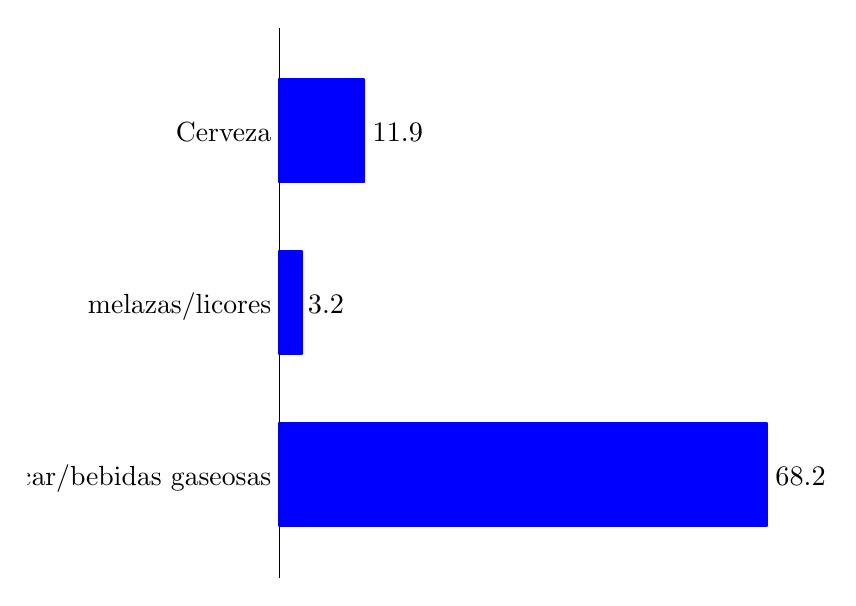
\begin{tikzpicture}[x=1pt,y=1pt]  % Created by tikzDevice version 0.9 on 2016-03-03 04:17:04
% !TEX encoding = UTF-8 Unicode
\definecolor{fillColor}{RGB}{255,255,255}
\path[use as bounding box,fill=fillColor,fill opacity=0.00] (0,0) rectangle (289.08,198.74);
\begin{scope}
\path[clip] (  0.00,  0.00) rectangle (289.08,198.74);

\path[] (  0.00,  0.00) rectangle (289.08,198.74);
\end{scope}
\begin{scope}
\path[clip] (  0.00,  0.00) rectangle (289.08,198.74);

\path[] ( 90.78,  0.00) rectangle (267.09,198.74);

\path[] ( 90.78, 37.26) --
	(267.09, 37.26);

\path[] ( 90.78, 99.37) --
	(267.09, 99.37);

\path[] ( 90.78,161.48) --
	(267.09,161.48);
\definecolor{drawColor}{RGB}{0,0,255}
\definecolor{fillColor}{RGB}{0,0,255}

\path[draw=drawColor,line width= 0.6pt,line join=round,fill=fillColor] ( 90.78, 18.63) rectangle (267.09, 55.90);

\path[draw=drawColor,line width= 0.6pt,line join=round,fill=fillColor] ( 90.78, 80.74) rectangle ( 99.05,118.00);

\path[draw=drawColor,line width= 0.6pt,line join=round,fill=fillColor] ( 90.78,142.85) rectangle (121.54,180.11);
\definecolor{drawColor}{RGB}{0,0,0}

\path[draw=drawColor,line width= 0.1pt,line join=round] ( 90.78,  0.00) -- ( 90.78,198.74);

\node[text=drawColor,anchor=base west,inner sep=0pt, outer sep=0pt, scale=  1.02] at (270.21, 33.29) {68.2};

\node[text=drawColor,anchor=base west,inner sep=0pt, outer sep=0pt, scale=  1.02] at (101.29, 95.40) {3.2};

\node[text=drawColor,anchor=base west,inner sep=0pt, outer sep=0pt, scale=  1.02] at (124.67,157.51) {11.9};

\path[] ( 90.78,  0.00) rectangle (267.09,198.74);
\end{scope}
\begin{scope}
\path[clip] (  0.00,  0.00) rectangle (289.08,198.74);

\path[] ( 90.78,  0.00) --
	( 90.78,198.74);
\end{scope}
\begin{scope}
\path[clip] (  0.00,  0.00) rectangle (289.08,198.74);
\definecolor{drawColor}{RGB}{0,0,0}

\node[text=drawColor,anchor=base east,inner sep=0pt, outer sep=0pt, scale=  1.00] at ( 88.03, 33.36) {azúcar/bebidas gaseosas};

\node[text=drawColor,anchor=base east,inner sep=0pt, outer sep=0pt, scale=  1.00] at ( 88.03, 95.46) {melazas/licores};

\node[text=drawColor,anchor=base east,inner sep=0pt, outer sep=0pt, scale=  1.00] at ( 88.03,157.57) {Cerveza};
\end{scope}
\begin{scope}
\path[clip] (  0.00,  0.00) rectangle (289.08,198.74);

\path[] ( 88.03, 37.26) --
	( 90.78, 37.26);

\path[] ( 88.03, 99.37) --
	( 90.78, 99.37);

\path[] ( 88.03,161.48) --
	( 90.78,161.48);
\end{scope}
  \end{tikzpicture}}%
{%
	INE y MAGA} %